\documentclass[UTF8,openany,12pt]{ctexbook}

\usepackage[a4paper,margin=2.6cm,bindingoffset=0.6cm,headheight=15pt]{geometry}
\usepackage{amsmath,amssymb,mathtools,amsthm}
\usepackage{bm}
\usepackage{graphicx}
\usepackage{booktabs,longtable,array,tabularx}
\usepackage{siunitx}
\usepackage[dvipsnames]{xcolor}
\usepackage[most]{tcolorbox}
\usepackage{enumitem}
\usepackage{listings}
\usepackage{hyperref}
\usepackage{bookmark}
\usepackage[capitalise,noabbrev]{cleveref}

\hypersetup{
  colorlinks=true,
  linkcolor=MidnightBlue,
  citecolor=ForestGreen,
  urlcolor=BrickRed,
  bookmarksnumbered=true
}

\setcounter{secnumdepth}{3}
\setcounter{tocdepth}{2}
\numberwithin{equation}{chapter}
\sisetup{detect-all,separate-uncertainty=true}

\pagestyle{headings}
\raggedbottom

\lstdefinestyle{bookpython}{
  language=Python,
  basicstyle=\ttfamily\small,
  keywordstyle=\color{MidnightBlue}\bfseries,
  commentstyle=\color{ForestGreen},
  stringstyle=\color{BrickRed},
  numbers=left,
  numberstyle=\tiny\color{gray},
  frame=single,
  breaklines=true,
  showstringspaces=false,
  columns=fullflexible
}

\crefname{equation}{式}{式}
\crefname{figure}{图}{图}
\crefname{table}{表}{表}
\crefname{chapter}{章}{章}
\crefname{section}{节}{节}

\newcommand{\ii}{\mathrm{i}}
\newcommand{\ee}{\mathrm{e}}
\newcommand{\dd}{\mathop{}\!\mathrm{d}}
\newcommand{\Tr}{\operatorname{Tr}}
\newcommand{\diag}{\operatorname{diag}}
\newcommand{\Var}{\operatorname{Var}}
\newcommand{\Cov}{\operatorname{Cov}}
\newcommand{\order}{\mathcal{O}}
\newcommand{\identity}{\mathbb{I}}
\newcommand{\hpsi}{\hat{\Psi}}
\newcommand{\hpsid}{\hat{\Psi}^{\dagger}}
\newcommand{\ha}{\hat a}
\newcommand{\had}{\hat a^{\dagger}}
\newcommand{\hb}{\hat b}
\newcommand{\hbd}{\hat b^{\dagger}}
\newcommand{\rhohat}{\hat\rho}
\newcommand{\Hhat}{\hat H}
\newcommand{\Ohat}{\hat O}
\newcommand{\Wigner}{W}
\newcommand{\qavg}[1]{\left\langle #1\right\rangle}
\newcommand{\ensavg}[1]{\mathbb{E}_{W}\!\left[#1\right]}
\newcommand{\comm}[2]{\left[#1,#2\right]}
\newcommand{\acomm}[2]{\left\{#1,#2\right\}}
\newcommand{\pder}[2]{\frac{\partial #1}{\partial #2}}
\newcommand{\fder}[2]{\frac{\delta #1}{\delta #2}}
\newcommand{\phasevec}{\bm z}
\newcommand{\orderparameter}{\rho_Q}
\newcommand{\ket}[1]{\left\lvert #1\right\rangle}
\newcommand{\bra}[1]{\left\langle #1\right\rvert}
\newcommand{\braket}[2]{\left\langle #1\middle\vert #2\right\rangle}
\newcommand{\mel}[3]{\left\langle #1\middle\vert #2\middle\vert #3\right\rangle}

\newtheorem{definition}{定义}[chapter]
\newtheorem{theorem}{定理}[chapter]
\newtheorem{proposition}{命题}[chapter]
\newtheorem{example}{例}[chapter]

\newtcolorbox{learningobjectives}{
  enhanced,breakable,colback=Blue!4,colframe=MidnightBlue,
  title={本章目标},fonttitle=\bfseries
}
\newtcolorbox{intuitionbox}{
  enhanced,breakable,colback=Green!4,colframe=ForestGreen,
  title={物理直觉},fonttitle=\bfseries
}
\newtcolorbox{derivationbox}{
  enhanced,breakable,colback=gray!4,colframe=black!65,
  title={关键推导},fonttitle=\bfseries
}
\newtcolorbox{numericalbox}{
  enhanced,breakable,colback=Cyan!4,colframe=TealBlue,
  title={数值实验},fonttitle=\bfseries
}
\newtcolorbox{warningbox}{
  enhanced,breakable,colback=Red!4,colframe=BrickRed,
  title={有效性警告},fonttitle=\bfseries
}
\newtcolorbox{chaptercheck}{
  enhanced,breakable,colback=Yellow!8,colframe=Orange,
  title={章末检查},fonttitle=\bfseries
}

\newenvironment{exercises}
  {\section*{习题}\addcontentsline{toc}{section}{习题}\begin{enumerate}[label=\textbf{\thechapter.\arabic*}]}
  {\end{enumerate}}


\title{维格纳相空间方法与玻色多体量子动力学\\[0.6em]
\large 从量子涨落、初态抽样到截断维格纳模拟}
\author{初稿}
\date{\today}

\hypersetup{
  pdftitle={维格纳相空间方法与玻色多体量子动力学},
  pdfsubject={Wigner 相空间与截断维格纳方法研究生教材},
  pdfauthor={初稿}
}



\begin{document}

\frontmatter
\maketitle
\chapter*{前言}
\addcontentsline{toc}{chapter}{前言}

多体量子动力学的困难并不只在于 Hilbert 空间随自由度指数增长，还在于研究者通常面对一个更具体的工作问题：初态已经给定，哈密顿量也已经写出，究竟怎样把它们转化成可以运行、可以验证、并能回到实验观测量的计算流程？本书围绕这一问题组织 Wigner 相空间方法与截断维格纳近似。

本书不把相空间方法描述成将量子力学“变成经典力学”的魔法。Wigner 函数是准概率分布，负值、算符排序和高阶 Moyal 导数都记录着经典概率论无法容纳的量子结构。TWA 所做的是在明确条件下保留初态的相空间涨落和领先的半经典动力学，同时舍弃一部分后续量子干涉。因此，任何应用章节都同时讲授计算方法和失效诊断。

全书由简单到复杂：单模谐振子建立符号和直觉，Kerr 振子暴露截断的代价，Bose--Hubbard 二聚体连接多模量子动力学，离散玻色场引出实际数值问题，最后以双分量凝聚体淬火说明如何构造 Bogoliubov 初态、传播随机场并诊断密度序与相干序。涉及数值的图表均由配套程序实际生成，而不是根据预期结论绘制。

这是一本方法教材，而不是对某个具体体系预设结论的论证。若模型、参数或有限尺寸证据不足，本书将结论停在证据能够支持的位置。

\chapter*{如何使用本书}
\addcontentsline{toc}{chapter}{如何使用本书}

本书既可以作为一门研究生课程的教材，也可以作为开展截断维格纳近似（以下简称 TWA）数值研究时的案头参考。全书的主线不是罗列相空间公式，而是反复回答同一组问题：量子态如何变成可抽样的初始分布，算符演化如何变成相空间轨迹，轨迹平均如何还原实验观测量，以及近似和数值离散在什么条件下仍然可信。读者在进入某一章以前，最好先明确自己要解决的是上述哪一个环节。

\section*{读者需要具备什么基础}

阅读本书需要熟悉本科量子力学中的态矢、密度算符、对易关系和谐振子，并能够使用傅里叶变换、常微分方程和基本概率统计。了解二次量子化、玻色凝聚和 Gross--Pitaevskii 方程会使第三、四部分更容易，但第10章仍从有限模式展开重新建立所需记号。涉及路径积分、随机微分方程或 Bogoliubov 理论的内容均在首次使用时给出必要背景。

读者不必在开始阅读前熟练掌握编程。不过，若希望复现数值实验，应具备基本的 Python 数组运算和绘图经验，并理解步长、网格、样本数与随机种子各自控制什么误差。附录C给出数值算法和测试规范，可以在阅读第12章前提前查阅。

\section*{五种建议阅读路线}

各章之间存在明确的依赖关系，但并非每位读者都需要从头顺序读到结尾。可以根据目标选择下列路线。

\begin{description}[style=nextline,leftmargin=2.2em,font=\bfseries]
  \item[系统学习路线]
  按照第1--18章顺序阅读。第一部分建立 Weyl--Wigner 表示，第二部分说明 TWA 从何而来以及为何失效，第三部分把单模方法推广到离散玻色场，第四部分完成双分量淬火案例，第五部分讨论开放系统、替代方法与研究工作流。这条路线适合一学期课程和首次系统接触相空间方法的读者。

  \item[快速开始 TWA 计算]
  先读第1、4、7和9章，掌握问题结构、排序修正、截断步骤和有效性边界；随后完整阅读第10--13章，依次完成模式截断、初态抽样、经典场传播和观测量重构。遇到推导细节时回查第2、3章及附录A。快速路线不能跳过第9章，因为“方程可以运行”并不等于 TWA 在目标时间尺度上有效。

  \item[偏重形式理论与推导]
  重点阅读第2、3、5--9章，并配合附录A、B。建议亲手推导谐振子、Kerr 振子和 Bose--Hubbard 二聚体的 Weyl 符号，再比较精确 Moyal 演化与截断后的 Liouville 流。第5章的二次体系是符号、归一化和传播器实现的基准，第6、8章则用精确小系统暴露非线性近似的误差来源。

  \item[双分量凝聚体与淬火动力学]
  在第1、4、7和9章之后，阅读第10--17章。第14章区分均匀组分耦合与具有动量转移的拉曼自旋轨道耦合；第15、16章研究线性化淬火、相位扩散和模式耦合；第17章集中讨论条纹序、有限尺寸标度及超固态判据。这里必须把动力学中出现条纹、存在相干峰和证明平衡态自发对称性破缺视为不同层次的命题。

  \item[数值实现与研究复现]
  先读第4、7、10--13章和附录B、C，再运行随书程序。对每个案例都应先复现默认基准，然后分别改变样本数、时间步长、空间网格、模式截止和随机种子；只有主要结论在相应收敛区间内稳定，才能把图像解释为物理结果。准备独立研究时，再用第9章和第18章选择精确对照、替代方法及失效诊断。
\end{description}

\section*{每一章应当怎样读}

每章开头的“本章目标”说明读完后应能完成的任务，而不是仅需记住的术语。建议按照下面四步使用一章内容。

\begin{enumerate}[label=\textbf{第\arabic*步},leftmargin=4.2em]
  \item \textbf{先定位问题。} 在阅读推导前写下本章的输入、输出和近似。例如，输入是密度算符还是 Bogoliubov 协方差，输出是单条轨迹还是正规排序关联函数。若无法说清这两点，复杂公式通常也难以正确使用。

  \item \textbf{沿计算链阅读。} 对每个模型追踪
  \[
    \begin{aligned}
      \text{量子态与哈密顿量}
      &\longrightarrow \text{Weyl 符号与初态抽样}\\
      &\longrightarrow \text{轨迹方程}\\
      &\longrightarrow \text{观测量估计器}\\
      &\longrightarrow \text{误差与有效性判断}.
    \end{aligned}
  \]
  不要只抄写中间的运动方程。漏掉初态的半量子噪声或末端的排序修正，都可能得到看似平滑但物理含义错误的结果。

  \item \textbf{完成最小验证。} 对解析章节检查一个可解极限；对数值章节至少检查维度、守恒量、步长收敛、网格或模式截止收敛以及统计误差。书中“数值实验”给出可复现基准，“有效性警告”指出即使程序无报错仍可能出现的系统偏差。

  \item \textbf{用章末问题闭环。} “章末检查”适合口头自测，习题用于补齐推导和实现细节。附录D提供提示与部分答案；建议先保留完整推导和失败尝试，再与提示比较，而不是从答案反推步骤。
\end{enumerate}

若把本书用于课程教学，可以把一次课分成“物理问题与表示”“核心推导”“数值或解析验证”三段。若用于自学，每章结束时应能用一页纸回答三个问题：本章作了什么近似；什么量可以与实验或精确结果比较；哪一个检验最可能推翻当前结论。

\section*{必须始终区分的平均与排序}

本书使用相似的尖括号或平均符号描述不同操作。它们不能互换：
\begin{equation*}
  \text{量子期望}\quad
  \qavg{\Ohat}=\Tr(\rhohat\Ohat),
  \qquad
  \text{Wigner 样本平均}\quad
  \ensavg{F}=\frac{1}{N_{\mathrm{s}}}
  \sum_{s=1}^{N_{\mathrm{s}}}F[\psi_s].
\end{equation*}
空间平均、时间平均和无序平均会在使用它们的章节中另行定义。一条 Wigner 轨迹不是一次完整的量子测量，也通常不等于量子期望；它是用于构造系综统计的相空间样本。

Wigner 平均天然给出对称排序量，而粒子数、密度和计数关联通常采用正规排序。最简单的单模例子是
\begin{equation*}
  \qavg{\had\ha}=\ensavg{|\alpha|^2}-\frac12.
\end{equation*}
在有限模式场中，$1/2$ 被局域投影核 $\delta_{\mathcal C}(x,x)/2$ 取代。因而，读者在记录任何数值观测量时，都应同时记录它的算符定义、排序约定和相空间估计器。第4章介绍单模修正，第10、13章给出场论版本，附录A汇总常用公式。

\section*{如何使用随书数值材料}

获得本书源码后，应从项目根目录运行程序。各章程序位于 \path{code/}，轻量数值结果位于 \path{data/}，生成的图位于 \path{figures/}。命令
\begin{lstlisting}[style=bookpython,numbers=none]
python code/run_all.py
\end{lstlisting}
会依次运行书中的九个数值基准，并把通过状态、运行时间和输出摘要写入 \path{data/test_summary.json}。单个脚本也可以独立运行，适合在修改参数后快速检查。实际 Python 可执行文件和依赖版本应由读者自己的环境记录；不能仅凭一张相似图像认定复现成功。

建议为每项研究建立四层记录：第一层保存模型参数、单位和随机种子；第二层保存代码版本及运行环境；第三层保存原始轨迹或足以重新计算观测量的数据；第四层保存制图脚本和最终统计量。正文图像用于说明物理结论，不替代原始数据和收敛证据。若修改算法、截止或估计器，应把修改后的结果与默认基准并列，而不是覆盖基准。

\section*{把本书方法用于新问题之前}

从本书案例迁移到新体系时，建议先回答以下问题：保留了哪些模式，舍弃了哪些模式；初态 Wigner 函数能否可靠抽样；Moyal 方程中删去了哪些高阶导数；占据数和演化时间是否处于受控范围；正规排序修正相对于物理信号有多大；结果是否通过样本、步长、网格和截止扫描；是否存在精确小系统、Bogoliubov 理论或其他多体方法可作交叉验证。

这些问题中任何一个没有答案，都不必立刻否定 TWA，但应降低结论强度并明确标注限制。尤其要避免三种常见推断：把单条轨迹的结构当作量子系综序，把有限尺寸中的峰当作热力学极限相变，以及把教学模型的参数趋势直接当作具体实验的定量预言。第9章提供系统的有效性审计，第17章讨论序参量和有限尺寸证据，第18章说明何时应改用正-$P$、张量网络、精确对角化或开放系统方法。

最后，本书所有连续场表达式都应理解为先在有限模式子空间或有限网格上定义，再讨论改变截止时的行为。增加网格点会同时增加真空半量子噪声，并不自动产生更精确的连续极限。读者若始终保留“表示---传播---估计---验证”这条主线，就能把本书当作一套可审计的研究流程，而不只是一组可调用的公式。

\tableofcontents
\chapter*{符号与约定}
\addcontentsline{toc}{chapter}{符号与约定}

本书同时使用有量纲的正则坐标与无量纲的模式正交分量。为避免把两者的
相空间测度、真空方差或 $\hbar$ 因子混在一起，统一采用
\begin{equation*}
  \comm{\hat x}{\hat p_x}=\ii\hbar,
  \qquad
  \comm{\hat Q}{\hat P}=\ii,
  \qquad
  \ha=\frac{\hat Q+\ii\hat P}{\sqrt2},
  \qquad
  \alpha=\frac{Q+\ii P}{\sqrt2}.
\end{equation*}
其中 $x,p_x$ 只表示有量纲的粒子坐标与动量，$Q,P$ 只表示单个正则玻色
模式的无量纲正交分量；因此 $\comm{\ha}{\had}=1$，且真空满足
$\Var(Q)=\Var(P)=1/2$。若某一局部推导令 $\hbar=1$，正文会明确说明。

场算符在连续表象中满足
\begin{equation*}
  \comm{\hpsi(x)}{\hpsid(x')}=\delta(x-x').
\end{equation*}
实际计算始终先选定有限模式子空间 $\mathcal C$，并以
$\mathcal P_{\mathcal C}$ 表示投影、以
$\delta_{\mathcal C}(x,x')$ 表示投影核。$M$ 表示保留模式数，$N_s$
表示独立 Wigner 轨迹数；周期均匀格点的长度、点数和间距分别为
$L,M,\Delta x=L/M$。离散模式、胞元模式与点值场的关系在第10章严格
固定。

全书把未扣除半量子的原始对称范数和粒子数算符的 Weyl 符号严格区分：
\begin{equation*}
  \mathcal N_{\mathrm{sym}}=\sum_{j=1}^{M}|\alpha_j|^2,
  \qquad
  N_W=(\hat N)_W=\mathcal N_{\mathrm{sym}}-\frac M2.
\end{equation*}
对正交格点的点值场，第一式等价于
$\mathcal N_{\mathrm{sym}}=\Delta x\sum_j|\psi_j|^2$。因此
$\mathcal N_{\mathrm{sym}}$ 可以是轨迹方程保持的原始模方和，物理粒子数则由
$\qavg{\hat N}=\ensavg{N_W}$ 给出；两者不得都简写为 $N_W$。

三类平均必须区分：
\begin{equation*}
  \qavg{\Ohat}=\Tr(\rhohat\Ohat),
  \qquad
  \ensavg{F}=\frac1{N_s}\sum_{r=1}^{N_s}F_r,
  \qquad
  \overline{F}^{\,x}=\frac1L\int_0^L F(x)\dd x .
\end{equation*}
前两者分别是量子期望和 Wigner 样本平均，最后一个仅表示空间平均。
一条轨迹的场值不是一次完整量子测量结果。

双分量章节采用自旋量
$\bm\psi=(\psi_L,\psi_R)^T$，总密度与自旋密度分别为
$n=|\psi_L|^2+|\psi_R|^2$ 和
$s=|\psi_L|^2-|\psi_R|^2$。为与场展开
$\delta\bm\psi=U\bm b-V^*\bm b^*$ 的负号一致，Bogoliubov--de Gennes（BdG）正能 Nambu 列统一写成
\begin{equation*}
  \bm w_\nu=\begin{pmatrix}\bm u_\nu\\-\bm v_\nu\end{pmatrix},
  \qquad
  \bar{\bm w}_\nu=\tau_x\bm w_\nu^*
  =\begin{pmatrix}-\bm v_\nu^*\\\bm u_\nu^*\end{pmatrix},
  \qquad
  S=\begin{pmatrix}U&-V^*\\-V&U^*\end{pmatrix}.
\end{equation*}
其中 $U=(\bm u_1,\ldots,\bm u_M)$、$V=(\bm v_1,\ldots,\bm v_M)$，
$\bar{\bm w}_\nu$ 是粒子--空穴伙伴，辛度量为
$\Sigma_z=\diag(\identity,-\identity)$。普通转置、Hermitian 共轭和复共轭
分别记为 $T$、$\dagger$ 和 $*$；粗体表示有限维向量或矩阵。

Fourier 变换在解析推导中采用连续归一化，在程序中采用附录A列出的幺正
离散约定。不同约定可以等价，但同一公式中的正变换、反变换、Parseval
关系和投影核必须成套使用。


\mainmatter

\part{从量子力学到相空间}
\chapter{从量子态到可计算动力学}
\label{ch:motivation}

\begin{learningobjectives}
完成本章后，读者应能：
\begin{enumerate}
  \item 把一个动力学问题写成初态 $\rhohat_0$、哈密顿量 $\Hhat$ 和观测量 $\Ohat$ 的三元组；
  \item 区分相空间表象、经典场近似和截断维格纳近似；
  \item 画出从初始 Wigner 分布到量子观测量的完整计算链；
  \item 为一项数值结论列出最低限度的验证证据。
\end{enumerate}
\end{learningobjectives}

\section{问题不是“解出波函数”}

教科书中的量子动力学常从 Schrödinger 方程开始：
\begin{equation}
  \ii\hbar\pder{}{t}\ket{\psi(t)}=\Hhat\ket{\psi(t)}.
  \label{eq:schrodinger}
\end{equation}
对于少数自由度，\cref{eq:schrodinger} 几乎就是问题的完整定义。然而，实际的多体问题通常不是要求写下整个 $\ket{\psi(t)}$，而是要求回答一个有限的问题，例如粒子数是否重新分配、相干性以什么时间尺度衰减、某个动量峰是否随系统尺寸保持，或者一个密度波序参量是否建立。

因此，更有操作性的起点是三元组
\begin{equation}
  \mathcal{P}=\bigl(\rhohat_0,\Hhat,\Ohat\bigr),
  \label{eq:problem-triple}
\end{equation}
其中 $\rhohat_0$ 给出初态，$\Hhat$ 给出演化规律，$\Ohat$ 给出最终要回答的问题。目标量为
\begin{equation}
  \qavg{\Ohat(t)}
  =\Tr\!\left[\rhohat_0\,ee^{\ii\Hhat t/\hbar}
  \Ohat\ee^{-\ii\Hhat t/\hbar}\right].
  \label{eq:heisenberg-expectation}
\end{equation}
这个表达式完全精确，但“写得出来”不等于“算得出来”。对于每个格点最多容纳 $n_{\max}$ 个玻色子的 $M$ 模系统，截断 Hilbert 空间的维数为 $(n_{\max}+1)^M$；即使利用总粒子数守恒，维数仍随 $M$ 和粒子数迅速增长。

\begin{intuitionbox}
多体数值方法的核心不是消灭量子复杂性，而是选择问题真正需要保存的信息。Wigner 方法保存相空间分布及其矩，而不显式保存完整的多体态矢量。
\end{intuitionbox}

\section{相空间表象改变了什么}

经典统计力学用概率密度 $P(q,p)$ 表示对初始条件的不确定性，并沿 Hamilton 方程传播每个样本。量子力学不能直接照搬这一做法，因为 $\hat q$ 与 $\hat p$ 不对易，也不存在同时给出二者任意精确取值的正概率分布。Wigner 在 1932 年引入的分布以实函数 $W(q,p)$ 编码密度算符，同时允许分布出现负值\cite{Wigner1932,Hillery1984}。

对采用本书归一化的单自由度系统，Wigner 表象满足
\begin{equation}
  \int\dd q\,\dd p\,W(q,p)=1,
  \qquad
  \qavg{\Ohat}=\int\dd q\,\dd p\,W(q,p)O_W(q,p),
  \label{eq:wigner-average-preview}
\end{equation}
其中 $O_W$ 是算符 $\Ohat$ 的 Weyl 符号。\cref{eq:wigner-average-preview} 看起来像经典统计平均，但两个细节使它仍然是量子力学：$W$ 未必非负，且 $O_W$ 不是把算符简单替换为数，而是由对称排序确定。

相空间表象本身是精确的变量变换。近似出现在我们怎样传播 $W$。精确传播由 Moyal 方程给出；对于至多二次的 Hamiltonian，它退化为经典 Liouville 方程；对于非线性相互作用，它还包含更高阶相空间导数。TWA 舍弃其中高于一阶漂移的项，把传播变成经典场轨迹系综\cite{Moyal1949,Polkovnikov2010}。

\section{本书的计算闭环}

给定\cref{eq:problem-triple}，一项完整的 Wigner/TWA 计算包含五步：
\begin{equation}
  (\rhohat_0,\Hhat,\Ohat)
  \longrightarrow W_0
  \longrightarrow \{\phasevec^{(s)}_0\}_{s=1}^{N_s}
  \longrightarrow \{\phasevec^{(s)}(t)\}_{s=1}^{N_s}
  \longrightarrow \qavg{\Ohat(t)}.
  \label{eq:book-pipeline}
\end{equation}

第一步选择有限模式或有限网格，并求初态的 Wigner 表象。第二步从 $W_0$ 生成 $N_s$ 个随机初值。若 $W_0$ 不是非负分布，这一步不能直接使用普通 Monte Carlo 抽样，必须采用近似、高斯重构或其他相空间表象。第三步对每个样本独立积分经典场方程。第四步把轨迹函数转化为 Weyl 排序的统计量。第五步根据目标算符的排序关系减去半量子等修正，得到正常排序或实验定义的观测量。

用符号写，若 $O_W$ 已知，则样本估计量为
\begin{equation}
  \widehat{\qavg{\Ohat(t)}}
  =\frac{1}{N_s}\sum_{s=1}^{N_s}
  O_W\!\left(\phasevec^{(s)}(t)\right).
  \label{eq:monte-carlo-estimator}
\end{equation}
有限样本误差通常按 $N_s^{-1/2}$ 缩小，但这只控制 Monte Carlo 误差，不控制 TWA 截断误差、空间离散误差和时间积分误差。

\section{三个层次不能混为一谈}

\subsection{精确 Wigner 表象}

密度算符与 Wigner 函数之间的变换是可逆的。在这一层次上，量子动力学没有被经典化；不对易性进入星积，非局域量子干涉进入 $W$ 的精细结构与负值区域。

\subsection{平均场轨迹}

平均场方法只传播一个典型复振幅或一个变分态。它可以准确描述高占据、涨落较弱的短时间动力学，但单条轨迹没有初态量子涨落的统计信息。确定性 Gross--Pitaevskii 方程本身不能给出由量子初态分布引起的轨迹间去相位。

\subsection{截断维格纳系综}

TWA 传播很多满足平均场型方程的轨迹，但初值由 Wigner 分布决定。非线性传播把初始涨落转换成观测量涨落、模式占据和系综去相位。因此，TWA 不等于“带随机数的 GPE”，随机数的协方差、基底和排序修正都由量子态决定。

\begin{warningbox}
“每条轨迹服从经典方程”不意味着“结果在任意时间都可靠”。非线性会形成越来越细的相空间结构，而被截去的高阶导数正负责其中一部分量子干涉。增加轨迹数只能降低抽样误差，不能修复系统性的截断误差。
\end{warningbox}

\section{一个最小例子：相干态谐振子}

考虑
\begin{equation}
  \Hhat=\hbar\omega\left(\had\ha+\frac12\right),
  \qquad \rhohat_0=\ket{\alpha_0}\bra{\alpha_0}.
\end{equation}
相干态的 Wigner 函数是以 $\alpha_0$ 为中心的正高斯分布。每个样本按
\begin{equation}
  \alpha^{(s)}(t)=\alpha^{(s)}(0)\ee^{-\ii\omega t}
  \label{eq:harmonic-trajectory-preview}
\end{equation}
旋转。由于 Hamiltonian 对正交分量至多二次，这不是近似，而是精确 Wigner 演化。若目标是粒子数，则不能直接把 $|\alpha|^2$ 当作 $\qavg{\had\ha}$，而要使用
\begin{equation}
  \qavg{\had\ha}
  =\ensavg{|\alpha|^2}-\frac12.
  \label{eq:number-half-preview}
\end{equation}
这里的 $1/2$ 是对称排序与正常排序之间的差，不是可选的数值修正。后续章节将从 Weyl 变换严格推出\cref{eq:number-half-preview}。

\section{怎样判断一个结果值得相信}

数值输出不是证据的终点。对本书中的每个计算，我们区分四类误差：
\begin{enumerate}
  \item \textbf{抽样误差}：改变轨迹数并报告置信区间；
  \item \textbf{积分误差}：改变时间步长并检查守恒量；
  \item \textbf{表示误差}：改变网格、模式数或局域占据截断；
  \item \textbf{方法误差}：与解析解、精确小系统或独立方法比较。
\end{enumerate}
前三类误差都很小，也不能自动证明 TWA 逼近了真实量子演化。方法误差必须通过具有重叠适用区的基准来估计。Kerr 振子与 Bose--Hubbard 二聚体将在后文承担这一任务。

\begin{chaptercheck}
面对一个新问题，先写清 $\rhohat_0$、$\Hhat$ 和 $\Ohat$，再决定是否使用 Wigner 方法。若目标观测量、初态抽样或排序修正有一项没有定义，计算闭环就尚未建立。
\end{chaptercheck}

\section*{本章小结}

Wigner 表象提供了从密度算符到相空间准分布的精确桥梁。TWA 在此基础上使用随机初值和经典漂移近似量子动力学。可信的工作流程必须同时说明初态怎样抽样、轨迹怎样传播、观测量怎样还原，以及近似怎样被独立验证。

\begin{exercises}
  \item 对两能级系统，说明为什么连续的 $(q,p)$ 相空间不是唯一自然选择，并列出一种替代表象。
  \item 设 $N_s$ 条独立轨迹给出样本 $O_s$。写出样本均值的标准误差估计，并说明它为什么不包含时间离散误差。
  \item 对相干态谐振子，利用\cref{eq:harmonic-trajectory-preview,eq:number-half-preview} 证明平均粒子数不随时间改变。
  \item 选取一个你关心的多体模型，把问题写成\cref{eq:problem-triple}，并为四类误差各提出一个检查。
\end{exercises}

\chapter{Weyl 变换与 Wigner 函数}
\label{ch:weyl-wigner}

\begin{learningobjectives}
完成本章后，读者应能：
\begin{enumerate}
  \item 从密度矩阵写出 Wigner 函数，并验证归一化和边缘分布；
  \item 计算简单算符的 Weyl 符号；
  \item 解释为什么 Wigner 平均对应对称排序；
  \item 正确抽样相干态和真空态的单模 Wigner 分布。
\end{enumerate}
\end{learningobjectives}

\section{从密度矩阵到实函数}

先从有量纲的位置--动量对 $\hat x,\hat p_x$ 出发，满足
\begin{equation}
  \comm{\hat x}{\hat p_x}=\ii\hbar.
\end{equation}
密度算符 $\rhohat$ 在坐标表象中的矩阵元 $\mel{x_1}{\rhohat}{x_2}$ 依赖两个坐标。引入中心坐标 $x=(x_1+x_2)/2$ 和相对坐标 $y=x_1-x_2$，再对 $y$ 作 Fourier 变换，得到 Wigner 函数
\begin{equation}
  W(x,p_x)=\frac{1}{2\pi\hbar}
  \int_{-\infty}^{\infty}\dd y\,
  \ee^{-\ii p_x y/\hbar}
  \mel{x+y/2}{\rhohat}{x-y/2}.
  \label{eq:wigner-coordinate-definition}
\end{equation}
这是 Wigner 准分布的标准坐标表象定义；不同归一化与量子光学中的常用复
振幅约定可与原始工作及综述交叉核对\cite{Wigner1932,Hillery1984}。
这里选择的系数使
\begin{equation}
  \int\dd x\,\dd p_x\,W(x,p_x)=\Tr\rhohat=1.
  \label{eq:wigner-normalization}
\end{equation}

\begin{derivationbox}
对\cref{eq:wigner-coordinate-definition} 先积分 $p_x$，利用
\[
  \int\dd p_x\,\ee^{-\ii p_x y/\hbar}=2\pi\hbar\,\delta(y),
\]
便得到 $\int\dd p_x\,W(x,p_x)=\mel{x}{\rhohat}{x}$。再积分 $x$ 即为迹。这个计算也说明 Wigner 函数的位置边缘分布是真正的概率密度。
\end{derivationbox}

Hermitian 性 $\rhohat^\dagger=\rhohat$ 保证 $W$ 为实函数。实函数并不意味着正函数；允许负值正是它能够同时编码不对易量信息的代价。另一方面，负值不是“量子性的必要条件”，真空态、相干态、热态和所有单模高斯态都可以具有处处非负的 Wigner 函数。

\section{边缘分布}

直接积分\cref{eq:wigner-coordinate-definition} 得
\begin{align}
  \int\dd p_x\,W(x,p_x)&=\mel{x}{\rhohat}{x},\\
  \int\dd x\,W(x,p_x)&=\mel{p_x}{\rhohat}{p_x}.
  \label{eq:wigner-marginals}
\end{align}
不过，\cref{eq:wigner-marginals} 不能解释为一次实验同时测得了确定的 $x$ 和 $p_x$；它只说明同一个准分布能够产生不同测量设置的边缘统计。有量纲的 $x$ 与 $p_x$ 不能在未选定尺度时直接相加；旋转正交分量将在下面引入无量纲变量后定义。

\section{Weyl 符号}

任意算符 $\hat A$ 的 Weyl 符号定义为
\begin{equation}
  A_W(x,p_x)=\int_{-\infty}^{\infty}\dd y\,
  \ee^{-\ii p_x y/\hbar}
  \mel{x+y/2}{\hat A}{x-y/2}.
  \label{eq:weyl-symbol-definition}
\end{equation}
密度算符的 Weyl 符号与 Wigner 函数相差归一化因子。两者配对给出迹公式
\begin{equation}
  \Tr(\rhohat\hat A)
  =\int\dd x\,\dd p_x\,W(x,p_x)A_W(x,p_x).
  \label{eq:weyl-trace-rule}
\end{equation}

Weyl 映射把完全对称排序的算符积映射为普通乘积。例如
\begin{align}
  (\hat x)_W&=x, & (\hat p_x)_W&=p_x,\\
  \left(\frac{\hat x\hat p_x+\hat p_x\hat x}{2}\right)_W&=xp_x,
  & (\hat x^2)_W&=x^2.
\end{align}
但一般情况下 $(\hat A\hat B)_W\neq A_WB_W$。算符乘积对应的星积将在第3章推导。

\section{玻色模式的复相空间}

对单个玻色模式，另行定义无量纲正交分量
\begin{equation}
  \ha=\frac{\hat Q+\ii\hat P}{\sqrt{2}},
  \qquad
  \alpha=\frac{Q+\ii P}{\sqrt{2}},
  \qquad \comm{\hat Q}{\hat P}=\ii,
  \qquad \comm{\ha}{\had}=1.
  \label{eq:mode-quadratures}
\end{equation}
物理系统若给出特征长度 $x_0$，一种常见选择是 $\hat Q=\hat x/x_0$、$\hat P=x_0\hat p_x/\hbar$；不同选择只是辛尺度变换，不能把两套变量的测度混用。复平面面积元为 $\dd^2\alpha=\dd(\Re\alpha)\dd(\Im\alpha)=\dd Q\dd P/2$。本书在复振幅表象中把 Wigner 函数归一化为
\begin{equation}
  \int\dd^2\alpha\,W(\alpha,\alpha^*)=1.
\end{equation}

现在可以定义可测的旋转正交分量
\begin{equation}
  \hat X_\theta=\hat Q\cos\theta+\hat P\sin\theta.
\end{equation}
对 Wigner 函数沿垂直于 $X_\theta$ 的方向作线积分，就得到该正交分量的概率分布；这也是量子层析中 Radon 反演的基础。

另一种常用定义从对称特征函数开始：
\begin{align}
  \chi_W(\lambda)&=\Tr\!\left[\rhohat\,
  \ee^{\lambda\had-\lambda^*\ha}\right],\\
  W(\alpha,\alpha^*)&=\frac{1}{\pi^2}
  \int\dd^2\lambda\,\chi_W(\lambda)
  \ee^{\lambda^*\alpha-\lambda\alpha^*}.
  \label{eq:wigner-characteristic}
\end{align}
指数中的位移算符同时包含 $\ha$ 和 $\had$，这正是对称排序出现的来源。

\section{真空态与相干态}

相干态满足 $\ha\ket{\alpha_0}=\alpha_0\ket{\alpha_0}$，其 Wigner 函数为
\begin{equation}
  W_{\alpha_0}(\alpha)
  =\frac{2}{\pi}\exp\!\left[-2|\alpha-\alpha_0|^2\right].
  \label{eq:coherent-wigner}
\end{equation}
真空态是 $\alpha_0=0$ 的特例。对\cref{eq:coherent-wigner} 的直接抽样为
\begin{equation}
  \alpha=\alpha_0+\frac{\xi_1+\ii\xi_2}{2},
  \qquad \xi_1,\xi_2\sim\mathcal{N}(0,1),
  \label{eq:coherent-sampling}
\end{equation}
其中两个实高斯变量相互独立。因此
\begin{equation}
  \ensavg{\alpha}=\alpha_0,
  \qquad
  \ensavg{|\alpha-\alpha_0|^2}=\frac12.
  \label{eq:vacuum-half-quantum}
\end{equation}
这个“半个量子”是正交分量真空噪声的相空间表示。

\begin{numericalbox}
抽样程序的第一项单元测试应检查\cref{eq:vacuum-half-quantum}，而不是只检查随机数看起来是否像高斯。若复噪声误写成 $(\xi_1+\ii\xi_2)/\sqrt{2}$，每个模式会被加入一个而不是半个量子的对称排序噪声。
\end{numericalbox}

\section{排序修正：粒子数的例子}

由 $\comm{\ha}{\had}=1$，
\begin{equation}
  \frac{\had\ha+\ha\had}{2}=\had\ha+\frac12.
\end{equation}
左侧是对称排序形式，其 Weyl 符号为 $|\alpha|^2$，所以
\begin{equation}
  (\had\ha)_W=|\alpha|^2-\frac12,
  \qquad
  \qavg{\had\ha}=\ensavg{|\alpha|^2}-\frac12.
  \label{eq:number-weyl-symbol}
\end{equation}
对相干态使用\cref{eq:coherent-sampling}，可得 $\ensavg{|\alpha|^2}=|\alpha_0|^2+1/2$，从而恢复 $\qavg{\had\ha}=|\alpha_0|^2$。

更高阶正规排序矩需要更多收缩项。例如
\begin{equation}
  (\had\had\ha\ha)_W
  =|\alpha|^4-2|\alpha|^2+\frac12.
  \label{eq:quartic-weyl-symbol}
\end{equation}
这类修正在接触相互作用和二阶关联函数中不可忽略。

\section{Wigner 函数能告诉我们什么}

归一化、边缘分布和矩使 Wigner 函数成为连接状态与实验统计的工具。它还满足纯度关系
\begin{equation}
  \Tr(\rhohat^2)=2\pi\hbar\int\dd x\,\dd p_x\,W(x,p_x)^2.
  \label{eq:wigner-purity}
\end{equation}
但不能仅凭一幅 Wigner 图断言动力学机制。负值可以见证某些非高斯非经典性；处处为正则不代表状态可以由经典统计完全解释。对多模场，完整 Wigner 函数存在于高维空间，实际计算主要依赖抽样和低阶边缘量，而不是绘制整个函数。

\begin{warningbox}
文献中的 Wigner 函数可能使用不同的面积元、$\pi$ 因子和正交分量归一化。引用抽样公式前必须同时核对：使用的是有量纲 $(x,p_x)$ 还是无量纲 $(Q,P)$、对易关系、$\alpha$ 的定义、积分测度和真空方差。
\end{warningbox}

\section*{本章小结}

Wigner 函数是密度矩阵相对坐标的 Fourier 变换，能够正确给出正交分量边缘分布。Weyl 符号把算符期望转化为相空间积分，并天然对应完全对称排序。相干态 Wigner 函数的真空宽度产生每模半量子噪声，正规排序观测量必须再作相应修正。

\begin{exercises}
  \item 从\cref{eq:wigner-coordinate-definition} 证明动量边缘分布，即\cref{eq:wigner-marginals} 的第二式。
  \item 验证\cref{eq:coherent-wigner} 在 $\dd^2\alpha$ 测度下归一化为 $1$。
  \item 使用对称排序推导\cref{eq:number-weyl-symbol}。
  \item 对真空态计算 $\ensavg{|\alpha|^4}$，再用\cref{eq:quartic-weyl-symbol} 验证 $\qavg{\had\had\ha\ha}=0$。
  \item 证明纯态的 Wigner 函数满足\cref{eq:wigner-purity} 右侧等于 $1$。
\end{exercises}

\chapter{星积、Moyal 括号与算符对应}
\label{ch:moyal}

\begin{learningobjectives}
完成本章后，读者应能：
\begin{enumerate}
  \item 用星积计算算符乘积的 Weyl 符号；
  \item 从 von Neumann 方程得到 Moyal 演化方程；
  \item 识别经典 Liouville 项和领先量子修正；
  \item 使用 Bopp 算符把主方程转换成相空间偏微分方程。
\end{enumerate}
\end{learningobjectives}

本章的实变量公式继续使用有量纲正则对 $(x,p_x)$，满足 $[\hat x,\hat p_x]=\ii\hbar$；进入复变量公式时，则使用第2章的无量纲 $\alpha=(Q+\ii P)/\sqrt2$。
星积与 Moyal 括号的原始表述见\cite{Moyal1949}；本章固定采用第2章的
归一化，避免把不同文献中的 $\hbar$ 与面积元约定混用。

\section{普通乘积为什么不够}

Weyl 映射保持线性，却不把算符乘积直接映射为普通函数乘积。记
\begin{equation*}
  \hat A\leftrightarrow A_W(x,p_x),
  \qquad
  \hat B\leftrightarrow B_W(x,p_x),
\end{equation*}
则
\begin{equation}
  (\hat A\hat B)_W=A_W\star B_W,
  \label{eq:star-product-correspondence}
\end{equation}
其中星积定义为
\begin{equation}
  A\star B
  =A\exp\!\left[
  \frac{\ii\hbar}{2}
  \left(
  \overleftarrow{\partial_x}\overrightarrow{\partial_{p_x}}
  -\overleftarrow{\partial_{p_x}}\overrightarrow{\partial_x}
  \right)\right]B.
  \label{eq:star-product}
\end{equation}
箭头说明导数作用在哪一侧。定义双向微分算符
\begin{equation}
  \Lambda=
  \overleftarrow{\partial_x}\overrightarrow{\partial_{p_x}}
  -\overleftarrow{\partial_{p_x}}\overrightarrow{\partial_x},
\end{equation}
则 $A\star B=A\exp(\ii\hbar\Lambda/2)B$。

把指数展开，得到
\begin{equation}
  A\star B=AB+\frac{\ii\hbar}{2}\{A,B\}_{\mathrm{PB}}
  +\order(\hbar^2),
  \label{eq:star-expansion}
\end{equation}
其中
\begin{equation}
  \{A,B\}_{\mathrm{PB}}
  =\pder{A}{x}\pder{B}{p_x}
  -\pder{A}{p_x}\pder{B}{x}
\end{equation}
是 Poisson 括号。星积由普通乘积、Poisson 几何和更高阶导数共同组成。

\begin{example}
取 $A=x$、$B=p_x$。因为二阶以上导数全部为零，
\begin{equation}
  x\star p_x=x p_x+\frac{\ii\hbar}{2},
  \qquad
  p_x\star x=p_x x-\frac{\ii\hbar}{2}.
\end{equation}
因此 $(\comm{\hat x}{\hat p_x})_W=x\star p_x-p_x\star x=\ii\hbar$。不对易性没有消失，而是进入星积。
\end{example}

\section{Moyal 括号}

算符对易子的 Weyl 符号定义 Moyal 括号：
\begin{align}
  \{A,B\}_{\mathrm{M}}
  &\equiv\frac{1}{\ii\hbar}(A\star B-B\star A)\\
  &=\frac{2}{\hbar}A
  \sin\!\left(\frac{\hbar}{2}\Lambda\right)B.
  \label{eq:moyal-bracket}
\end{align}
展开正弦可见
\begin{equation}
  \{A,B\}_{\mathrm{M}}
  =\{A,B\}_{\mathrm{PB}}
  -\frac{\hbar^2}{24}A\Lambda^3B
  +\order(\hbar^4).
  \label{eq:moyal-expansion}
\end{equation}
经典极限不是简单令 $\hbar=0$，而是要求高阶导数项相对于 Poisson 项可忽略。若 Wigner 函数在相空间中形成很细的振荡结构，即使 $\hbar$ 数值很小，高阶导数也可能变得重要。

\section{从 von Neumann 方程到 Wigner 演化}

闭合系统的密度算符满足
\begin{equation}
  \pder{\rhohat}{t}=-\frac{\ii}{\hbar}\comm{\Hhat}{\rhohat}.
  \label{eq:von-neumann}
\end{equation}
对\cref{eq:von-neumann} 作 Weyl 变换，利用\cref{eq:star-product-correspondence}，得到精确的 Moyal 方程
\begin{equation}
  \pder{W}{t}=\{H_W,W\}_{\mathrm{M}}.
  \label{eq:moyal-evolution}
\end{equation}
第一项是经典 Liouville 流，后续奇数阶导数包含量子修正。

对
\begin{equation}
  H_W(x,p_x)=\frac{p_x^2}{2m}+V(x),
\end{equation}
\cref{eq:moyal-evolution} 可写成
\begin{equation}
  \pder{W}{t}
  =-\frac{p_x}{m}\pder{W}{x}
  +\sum_{\ell=0}^{\infty}
  \frac{(-1)^\ell}{(2\ell+1)!}
  \left(\frac{\hbar}{2}\right)^{2\ell}
  \frac{\dd^{2\ell+1}V}{\dd x^{2\ell+1}}
  \frac{\partial^{2\ell+1}W}{\partial p_x^{2\ell+1}}.
  \label{eq:moyal-potential-series}
\end{equation}
当 $V$ 至多为二次多项式时，$V^{(3)}$ 及更高导数全部为零，精确量子传播便与经典 Liouville 传播一致。准确条件是哈密顿量的 Weyl 符号对全部相空间变量至多二次，而不只是“势能看起来像抛物线”。

把 Moyal 方程写成守恒流形式、检验归一化或推导矩方程时都使用了分部积分。对无界相空间，必须要求 $W$ 及所需阶数的导数在无穷远衰减得足够快，使边界通量为零；对周期相空间，边界项因周期性相消。若数值计算只保留有限相空间盒，则吸收、反射或周期边界会改变方程，不能在未检查边界概率质量的情况下沿用这些推导。

\section{非线性怎样产生高阶导数}

考虑四次势
\begin{equation}
  V(x)=\frac{\lambda}{4}x^4.
\end{equation}
因为 $V'''(x)=6\lambda x$ 且五阶以上导数为零，精确方程为
\begin{equation}
  \pder{W}{t}
  =-\frac{p_x}{m}\pder{W}{x}
  +\lambda x^3\pder{W}{p_x}
  -\frac{\hbar^2\lambda x}{4}\frac{\partial^3W}{\partial p_x^3}.
  \label{eq:quartic-wigner-evolution}
\end{equation}
前两项沿经典非线性轨迹剪切分布，第三项不能表示成普通确定性轨迹的概率守恒流。舍弃第三项便得到这一模型的截断 Wigner 演化。

\begin{intuitionbox}
非线性先把一个平滑相空间云团拉伸和折叠，再使分布出现越来越细的结构。精确量子项对这些结构敏感。TWA 在结构仍比量子相空间尺度粗时较有希望，在干涉条纹和回复形成后通常失效。
\end{intuitionbox}

\section{Bopp 算符：另一条推导路线}

与其每次显式展开星积，也可以用 Bopp 对应规则。对坐标变量，
\begin{align}
  \hat x\rhohat&\leftrightarrow
  \left(x+\frac{\ii\hbar}{2}\partial_{p_x}\right)W,
  &\rhohat\hat x&\leftrightarrow
  \left(x-\frac{\ii\hbar}{2}\partial_{p_x}\right)W,\\
  \hat p_x\rhohat&\leftrightarrow
  \left(p_x-\frac{\ii\hbar}{2}\partial_x\right)W,
  &\rhohat\hat p_x&\leftrightarrow
  \left(p_x+\frac{\ii\hbar}{2}\partial_x\right)W.
  \label{eq:bopp-real}
\end{align}
对玻色复振幅，令 $\alpha$ 与 $\alpha^*$ 在微分时相互独立，则
\begin{align}
  \ha\rhohat&\leftrightarrow
  \left(\alpha+\frac12\partial_{\alpha^*}\right)W,
  &\rhohat\ha&\leftrightarrow
  \left(\alpha-\frac12\partial_{\alpha^*}\right)W,\\
  \had\rhohat&\leftrightarrow
  \left(\alpha^*-\frac12\partial_\alpha\right)W,
  &\rhohat\had&\leftrightarrow
  \left(\alpha^*+\frac12\partial_\alpha\right)W.
  \label{eq:bopp-complex}
\end{align}
把哈密顿量或 Lindblad 主方程左右两侧的算符依次替换为\cref{eq:bopp-real,eq:bopp-complex}，即可得到 Wigner 偏微分方程。

\section{从偏微分方程到随机过程}

标准 Fokker--Planck 方程只含一阶和二阶导数：
\begin{equation}
  \pder{W}{t}
  =-\partial_i(A_iW)
  +\frac12\partial_i\partial_j(D_{ij}W).
  \label{eq:fokker-planck}
\end{equation}
当扩散矩阵可以适当分解时，\cref{eq:fokker-planck} 与随机微分方程对应。一阶项给出漂移，二阶项给出演化过程中持续注入的噪声。闭合、幺正、含四次相互作用的玻色系统在 Wigner 表象中通常出现一阶和三阶导数；TWA 丢弃三阶项后只剩确定性漂移，因此量子噪声只通过初始抽样进入。开放系统则可能保留二阶扩散，演化过程中仍有随机噪声。

\begin{warningbox}
“TWA 轨迹是确定性的”只适用于截断后的闭合幺正模型。含 Lindblad 损耗、测量或热浴时，Wigner 方程可以产生真正的二阶扩散，轨迹方程也会含随时间变化的噪声。
\end{warningbox}

\section{矩方程为何有时比整个分布更可靠}

在上一节说明的零边界通量条件下，高阶导数对低阶多项式矩的直接贡献可能因分部积分而消失。例如\cref{eq:quartic-wigner-evolution} 中的三阶 $p_x$ 导数不直接改变 $p_x^0,p_x^1,p_x^2$ 矩。然而，非线性会使低阶矩与更高阶矩耦合，高阶结构随后仍可能反馈回来。因此，某个低阶观测量在一段时间内准确，不代表完整 Wigner 函数或所有高阶关联都同样准确。

\begin{chaptercheck}
看到“经典轨迹”时，检查它来自精确的二次哈密顿量，还是来自对高阶 Moyal 导数的截断；看到“随机轨迹”时，检查噪声只在初态出现，还是由二阶扩散在演化中持续产生。
\end{chaptercheck}

\section*{本章小结}

星积保存了算符乘法和不对易性，Moyal 括号把 von Neumann 方程精确转写为相空间演化。Poisson 括号是其领先项，非线性哈密顿量产生高阶导数。TWA 的核心数学操作正是舍弃无法由普通轨迹表示的高阶项，而 Bopp 算符提供了对具体玻色哈密顿量进行这一推导的实用途径。

\begin{exercises}
  \item 使用\cref{eq:star-product} 计算 $x^2\star p_x^2$，保留全部非零项。
  \item 证明 Moyal 括号满足反对称性，并验证 $\{x,p_x\}_{\mathrm{M}}=1$。
  \item 从\cref{eq:moyal-potential-series} 推导四次势的\cref{eq:quartic-wigner-evolution}。
  \item 使用 Bopp 规则重新推导 $(\had\ha)_W=|\alpha|^2-1/2$。
  \item 对六次势 $V(x)=gx^6/6$，写出 Wigner 演化中最高阶的 $p_x$ 导数。
\end{exercises}

\chapter{常见量子态、非经典性与观测量}
\label{ch:states-observables}

\begin{learningobjectives}
完成本章后，读者应能：
\begin{enumerate}
  \item 写出相干态、热态、压缩高斯态和 Fock 态的 Wigner 函数；
  \item 根据协方差矩阵抽样多模高斯态；
  \item 区分 Wigner 负值、量子性和普通概率可抽样性；
  \item 把等时正规排序观测量转换为 Wigner 样本估计量。
\end{enumerate}
\end{learningobjectives}

\section{选择初态就是选择物理假设}

在 TWA 中，初态不是给平均场加一点任意噪声。初态的粒子数涨落、相位涨落、模间关联和反常关联都由 $\rhohat_0$ 决定。两个具有相同平均粒子数的状态，若一个是相干态、另一个是数态，其长期相位扩散可以完全不同。因此，抽样算法必须从态的矩或协方差出发，而不能只匹配一条平均密度曲线。

\section{相干态与热态}

第2章已经得到相干态
\begin{equation}
  W_{\alpha_0}(\alpha)=\frac{2}{\pi}
  \exp[-2|\alpha-\alpha_0|^2].
\end{equation}
它的位置由 $\alpha_0$ 决定，宽度固定为真空宽度。相干态粒子数服从 Poisson 分布，满足
\begin{equation}
  \qavg{\hat n}=|\alpha_0|^2,
  \qquad
  \Var(\hat n)=|\alpha_0|^2.
\end{equation}
如果实际制备固定总粒子数，直接使用相干态会额外引入全局数涨落；是否可接受取决于目标观测量是否对该涨落敏感。

平均热占据为 $\bar n$ 的单模热态具有
\begin{equation}
  W_{\mathrm{th}}(\alpha)
  =\frac{2}{\pi(2\bar n+1)}
  \exp\!\left[-\frac{2|\alpha|^2}{2\bar n+1}\right].
  \label{eq:thermal-wigner}
\end{equation}
其直接抽样为
\begin{equation}
  \alpha=\sqrt{\frac{\bar n+1/2}{2}}
  (\xi_1+\ii\xi_2),
  \qquad \xi_j\sim\mathcal{N}(0,1).
  \label{eq:thermal-sampling}
\end{equation}
于是 $\ensavg{|\alpha|^2}=\bar n+1/2$，减去排序修正后恢复 $\qavg{\hat n}=\bar n$。

\section{高斯态与协方差矩阵}

连续变量高斯态的辛空间形式、物理性条件与 Williamson 分解可参见综述
\cite{Weedbrook2012}；这里仅保留后续 Wigner 抽样直接需要的结果。

对 $M$ 个模式，把正交分量排列为
\begin{equation}
  \hat{\bm R}=(\hat Q_1,\hat P_1,\ldots,\hat Q_M,\hat P_M)^{\mathsf T}.
\end{equation}
定义均值和对称协方差
\begin{align}
  d_j&=\qavg{\hat R_j},\\
  V_{jk}&=\frac12\qavg{
  \acomm{\hat R_j-d_j}{\hat R_k-d_k}}.
  \label{eq:gaussian-covariance}
\end{align}
采用第2章的无量纲约定 $\comm{\hat Q_j}{\hat P_k}=\ii\delta_{jk}$ 时，物理协方差必须满足
\begin{equation}
  V+\frac{\ii}{2}\Omega\succeq0,
  \qquad
  \Omega=\bigoplus_{j=1}^{M}
  \begin{pmatrix}0&1\\-1&0\end{pmatrix}.
  \label{eq:uncertainty-matrix}
\end{equation}
高斯态的 Wigner 函数就是均值为 $\bm d$、协方差为 $V$ 的普通多元高斯：
\begin{equation}
  W(\bm R)=\frac{1}{(2\pi)^M\sqrt{\det V}}
  \exp\!\left[-\frac12(\bm R-\bm d)^{\mathsf T}
  V^{-1}(\bm R-\bm d)\right].
  \label{eq:multimode-gaussian-wigner}
\end{equation}
若 $V=LL^{\mathsf T}$，则
\begin{equation}
  \bm R=\bm d+L\bm\xi,
  \qquad \bm\xi\sim\mathcal{N}(\bm0,I)
  \label{eq:gaussian-cholesky-sampling}
\end{equation}
给出直接抽样。对合法的有限能量量子协方差，$V$ 是正定矩阵，通常可取 Cholesky 因子。纯高斯态只意味着所有辛本征值等于 $1/2$，并不意味着 $V$ 奇异；真正的数值病态来自强压缩或变量尺度失衡，使普通特征值跨越很多数量级。此时可使用对称特征分解构造平方根，但任何特征值裁剪都必须记录并回测其对目标矩的影响。

\subsection{单模压缩真空}

本书固定约定：$r>0$ 时 $Q$ 正交分量被压缩。此时
\begin{equation}
  V=\frac12
  \begin{pmatrix}
    \ee^{-2r}&0\\
    0&\ee^{2r}
  \end{pmatrix}.
  \label{eq:squeezed-covariance}
\end{equation}
一个正交分量的噪声低于真空，另一个按不确定关系增大。该态具有明确的量子压缩，却仍有处处非负的 Wigner 函数。这再次说明“Wigner 负值”等价于“量子性”的说法过强。

\subsection{模间关联}

两模压缩态的协方差矩阵含非零的模间块。若只按每个模式的边缘方差独立抽样，就会丢掉 $\qavg{\ha_k\ha_{-k}}$ 一类反常关联。淬火后的 Bogoliubov 初态正需要保留这种 $k$ 与 $-k$ 的关联；第15章将给出从准粒子变换构造 $V$ 的方法。

\begin{numericalbox}
高斯抽样至少检查三项：样本均值与 $\bm d$ 的偏差、样本协方差与 $V$ 的矩阵范数误差，以及 $V+\ii\Omega/2$ 的最小特征值。只检查每个对角方差不能发现模间关联丢失。
\end{numericalbox}

\subsection{高斯矩匹配的适用边界}

若目标态本身是高斯态，均值 $\bm d$ 与协方差 $V$ 唯一确定其全部等时矩，\cref{eq:gaussian-cholesky-sampling} 是精确初态抽样。若目标态非高斯，用相同的 $\bm d,V$ 构造高斯分布只保证一、二阶对称矩一致；它不保证粒子数分布、四阶关联、稀有尾部、Wigner 负值或相位干涉一致。

这种差别在非线性演化中不会停留在高阶矩。四次哈密顿量会使低阶矩方程与更高阶矩耦合，所以初始时一、二阶矩相同的两个状态，随后的一、二阶观测量也可能分离。采用高斯矩匹配时必须同时声明：匹配了哪些矩、目标观测量和时间窗口、与精确小系统的比较，以及结论对替代匹配方案是否稳定。不能把“协方差回测通过”写成“目标非高斯态已被精确表示”。

\section{Fock 态与 Wigner 负值}

粒子数态 $\ket{n}$ 的单模 Wigner 函数为
\begin{equation}
  W_n(\alpha)=\frac{2}{\pi}(-1)^n
  L_n(4|\alpha|^2)\ee^{-2|\alpha|^2},
  \label{eq:fock-wigner}
\end{equation}
其中 $L_n$ 是 Laguerre 多项式。除真空外，分布通常含正负交替的环，因此不能把\cref{eq:fock-wigner} 直接当作概率密度生成等权样本。

若 $Z_W=\int\dd^2\alpha\,|W(\alpha)|$ 有限，可定义
\begin{equation}
  P_{|W|}(\alpha)=\frac{|W(\alpha)|}{Z_W},
  \qquad s(\alpha)=\operatorname{sgn}W(\alpha),
\end{equation}
相应的积分估计器为
\begin{equation}
  \int\dd^2\alpha\,W(\alpha)O_W(\alpha)
  =Z_W\mathbb{E}_{|W|}[sO_W].
\end{equation}
这在数学上是无偏的符号重加权，却不是正 Wigner 抽样。平均符号满足
\begin{equation}
  \mathbb{E}_{|W|}[s]=\frac{1}{Z_W};
\end{equation}
当它很小时，所需样本数会急剧增加。更重要的是，这一重加权只处理初态
积分的负权重，并不会补回 TWA 随后舍弃的高阶 Moyal 动力学。

实际工作中有四种选择：在符号问题可控的小系统中使用上述重加权；使用能够处理复权重或扩展相空间的表示；构造只匹配目标低阶矩的近似正分布；或者直接使用精确态作为基准。矩匹配不是精确表示，必须按上一小节说明其边界。

猫态
\begin{equation}
  \ket{\psi_{\mathrm{cat}}}\propto
  \ket{\alpha_0}+\ee^{\ii\phi}\ket{-\alpha_0}
\end{equation}
的 Wigner 函数由两个高斯峰和中间的干涉条纹组成。若只抽样两个峰的经典混合，就会保留“在左或在右”的统计，却丢失相干叠加。Wigner 图中最细的干涉条纹也往往最先暴露半经典截断的局限。

\section{三种常用相空间分布}

不同相空间表示对应不同算符排序：
\begin{center}
\begin{tabular}{lll}
\toprule
表示 & 典型排序 & 主要特征 \\
\midrule
Glauber--Sudarshan $P$ & 正规排序 & 可能比普通函数更奇异 \\
Wigner $W$ & 对称排序 & 实函数，但可为负 \\
Husimi $Q$ & 反正规排序 & 始终非负，但额外平滑 \\
\bottomrule
\end{tabular}
\end{center}
不存在对所有问题都最优的表示。Wigner 表象的优势是漂移方程常接近经典场动力学，且高占据玻色系统的半量子修正清楚；它的限制是非正初态难以直接抽样，非线性演化又会产生高阶导数。
更一般的高斯算符表示可以扩展普通正概率抽样的范围，但其变量、权重和
稳定性条件与本章的 Wigner 高斯抽样不同\cite{Corney2003}。

\section{等时观测量的估计器}

对单模玻色子，常用估计器包括
\begin{align}
  \qavg{\hat n}
  &=\ensavg{|\alpha|^2-\frac12},\\
  \qavg{\hat n(\hat n-1)}
  &=\ensavg{|\alpha|^4-2|\alpha|^2+\frac12},
  \label{eq:wigner-factorial-moments}
\end{align}
从而
\begin{equation}
  g^{(2)}=
  \frac{\qavg{\had\had\ha\ha}}
  {\qavg{\had\ha}^2}.
\end{equation}
对不同模式 $j\neq k$，算符彼此对易，但每个同模的产生湮灭配对仍需排序修正。连续场中的 $1/2$ 会变成含网格尺度的 $1/(2\Delta x)$，第10章将详细推导。

以上规则直接适用于单一时刻的对称排序量。多时关联如 $\qavg{\had(t_1)\ha(t_2)}$ 不能总是把两个轨迹值直接相乘；时间排序、对易子和响应修正可能参与。若目标是谱函数或响应函数，必须从所需的时间排序重新推导估计器。

\begin{warningbox}
状态抽样正确，不代表观测量估计器自动正确。初态分布、动力学方程和算符排序是三项独立输入；任何一项使用了另一种相空间约定，最终结果都可能相差一个随模式数累积的真空修正。
\end{warningbox}

\section*{本章小结}

相干态和热态可以逐模直接抽样，一般高斯态应由完整协方差矩阵抽样。压缩态说明正 Wigner 函数仍能代表量子态，Fock 态和猫态则展示普通概率抽样的限制。等时观测量必须从 Weyl 符号构造；正规排序、多时排序和连续场极限需要分别处理。

\begin{exercises}
  \item 用\cref{eq:thermal-sampling} 计算 $\ensavg{|\alpha|^2}$ 和 $\ensavg{|\alpha|^4}$，验证热态的 $g^{(2)}=2$。
  \item 验证压缩真空协方差\cref{eq:squeezed-covariance} 饱和不确定关系。
  \item 对给定的 $4\times4$ 两模协方差矩阵，写出检查其物理性的步骤和抽样算法。
  \item 计算 $n=1$ Fock 态 Wigner 函数在 $\alpha=0$ 处的值，并解释为什么不能直接作正概率抽样。
  \item 比较相干态与固定粒子数态作为双阱初态时，总粒子数方差的差别，并讨论它可能怎样影响相位扩散。
\end{exercises}


\part{从精确演化到截断维格纳近似}
\chapter{二次哈密顿量的精确相空间流}
\label{ch:quadratic}

\begin{learningobjectives}
完成本章后，读者应能：
\begin{enumerate}
  \item 证明二次哈密顿量的 Wigner 演化严格等于经典 Liouville 演化；
  \item 用辛矩阵传播相空间均值和协方差；
  \item 区分“高斯态保持高斯”和“任意 Wigner 函数按线性流精确搬运”；
  \item 用守恒量、均值和协方差检验数值传播程序。
\end{enumerate}
\end{learningobjectives}

\section{一般二次哈密顿量}

二次玻色哈密顿量与连续变量高斯态的辛演化属于同一线性正则结构；
较完整的连续变量量子信息表述可参见\cite{Weedbrook2012}。

沿用第2章的无量纲模式正交分量，把 $M$ 模写成 $2M$ 维列向量
\begin{equation}
  \hat{\bm R}=(\hat Q_1,\hat P_1,\ldots,\hat Q_M,\hat P_M)^T,
\end{equation}
满足
\begin{equation}
  \comm{\hat R_j}{\hat R_k}=\ii\Omega_{jk}.
\end{equation}
一般的时变二次哈密顿量可写成频率单位的形式
\begin{equation}
  \Hhat(t)=\hbar\left[
  \frac12\hat{\bm R}^{\mathsf T}G(t)\hat{\bm R}
  +\bm h(t)^{\mathsf T}\hat{\bm R}+c(t)\right],
  \label{eq:quadratic-hamiltonian}
\end{equation}
其中 $G=G^{\mathsf T}$，$G$ 与 $\bm h$ 的量纲是频率。由于 Weyl 对称化，频率函数 $\mathcal H_W\equiv H_W/\hbar$ 就是把 $\hat{\bm R}$ 替换为 $\bm R$ 后的括号内二次函数。若改用有量纲的坐标--动量，则应把相应尺度和 $1/\hbar$ 一并恢复，不能与本段的 $G$ 直接混用。

Moyal 展开中的 $\Lambda^3$ 及更高项至少需要哈密顿量的三阶导数，因此全部为零。精确 Wigner 方程退化为
\begin{equation}
  \pder{W}{t}=\{\mathcal H_W,W\}_{\mathrm{PB}}.
  \label{eq:quadratic-liouville}
\end{equation}
它的特征线满足经典 Hamilton 方程
\begin{equation}
  \dot{\bm R}=\Omega\bigl[G(t)\bm R+\bm h(t)\bigr].
  \label{eq:linear-hamilton-equation}
\end{equation}
这里没有作 TWA 截断；经典形式来自 Moyal 级数精确终止。

\begin{intuitionbox}
二次哈密顿量不能在相空间中产生新的细尺度折叠。它只对已有分布作旋转、剪切、压缩和平移。因此，即使初态是带负值的 Fock 态 Wigner 函数，其精确演化仍可由同一线性辛流搬运。
\end{intuitionbox}

\section{辛传播矩阵}

齐次部分的基解矩阵 $S(t,t_0)$ 满足
\begin{equation}
  \pder{S(t,t_0)}{t}=\Omega G(t)S(t,t_0),
  \qquad S(t_0,t_0)=I.
\end{equation}
解可写成
\begin{equation}
  \bm R(t)=S(t,t_0)\bm R(t_0)+\bm r_c(t),
  \label{eq:affine-symplectic-flow}
\end{equation}
其中 $\bm r_c$ 由驱动 $\bm h$ 决定。传播保持对易关系，因而
\begin{equation}
  S\Omega S^{\mathsf T}=\Omega.
  \label{eq:symplectic-condition}
\end{equation}
满足\cref{eq:symplectic-condition} 的矩阵称为辛矩阵。

对均值 $\bm d$ 和协方差 $V$，传播规则为
\begin{align}
  \bm d(t)&=S\bm d(t_0)+\bm r_c(t),\\
  V(t)&=SV(t_0)S^{\mathsf T}.
  \label{eq:gaussian-moment-propagation}
\end{align}
若初态为高斯态，\cref{eq:gaussian-moment-propagation} 已经给出全部状态信息；若初态非高斯，均值和协方差仍按该式演化，但不能由它们重建完整状态。

\section{谐振子的相空间旋转}

\begin{equation}
  \Hhat=\hbar\omega\left(\had\ha+\frac12\right)
  =\frac{\hbar\omega}{2}(\hat Q^2+\hat P^2).
\end{equation}
Hamilton 方程为 $\dot Q=\omega P$、$\dot P=-\omega Q$，所以
\begin{equation}
  \begin{pmatrix}Q(t)\\P(t)\end{pmatrix}
  =
  \begin{pmatrix}
    \cos\omega t&\sin\omega t\\
    -\sin\omega t&\cos\omega t
  \end{pmatrix}
  \begin{pmatrix}Q(0)\\P(0)\end{pmatrix}.
  \label{eq:harmonic-symplectic-rotation}
\end{equation}
复振幅因此满足 $\alpha(t)=\alpha(0)\ee^{-\ii\omega t}$。相干态 Wigner 云团作刚性旋转，真空宽度不变，粒子数估计量 $|\alpha|^2-1/2$ 沿每条轨迹都守恒。

\begin{figure}[htbp]
  \centering
  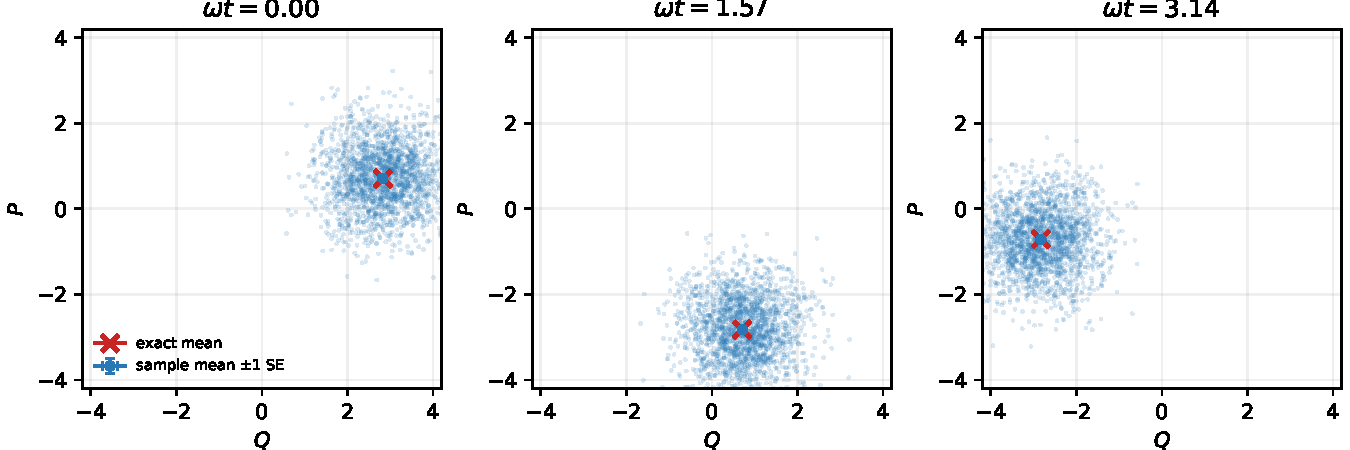
\includegraphics[width=0.94\textwidth]{figures/ch05/harmonic_wigner_rotation.pdf}
  \caption[谐振子二次流的 Wigner 样本基准]{相干态 Wigner 样本在谐振子二次哈密顿量下的精确旋转，参数为 $\alpha_0=2+0.5\ii$、$\omega=1$。蓝点为 $2000$ 条可视化轨迹的截面，圆点及误差棒为全部 $20000$ 条轨迹给出的样本均值及其 $\pm1$ 标准误，红叉为解析均值。该基准只检验可精确抽样的高斯初态与二次传播；图由 \texttt{code/ch05\_quadratic/harmonic\_wigner.py} 实际计算。}
  \label{fig:harmonic-wigner-rotation}
\end{figure}

\section{实际数值验证}

\cref{fig:harmonic-wigner-rotation} 使用 $\alpha_0=2+0.5\ii$、$\omega=1$ 和固定随机种子。样本通过
\begin{equation}
  \alpha^{(s)}(0)=\alpha_0+\frac{\xi_1^{(s)}+\ii\xi_2^{(s)}}{2}
\end{equation}
生成，再用解析旋转传播。程序输出的验证结果为
\begin{align}
  \max_t|\overline\alpha(t)-\alpha_0\ee^{-\ii t}|
  &=5.51\times10^{-3},\\
  \widehat{\qavg{\hat n}}&=4.25275,
  \qquad \qavg{\hat n}_{\mathrm{exact}}=4.25.
\end{align}
三个抽查时刻的 $Q,P$ 样本方差位于 $0.4985$ 至 $0.5051$，与真空方差 $1/2$ 相容。数据保存在 \texttt{data/ch05/harmonic\_wigner\_metrics.json}。

这些偏差来自有限样本，不是动力学截断。若把轨迹数扩大四倍，均值误差的典型尺度应约缩小一半。由于传播使用解析解，时间离散误差在本实验中为零。

\begin{numericalbox}
二次模型是测试 TWA 软件的首选：初态抽样、漂移、观测量排序和解析答案可以同时检查。若代码不能在此处保持协方差和二次守恒量，就不应直接用于非线性多体模型。
\end{numericalbox}

\section{自由膨胀、剪切与压缩}

这里临时回到有量纲的位置--动量对：自由粒子哈密顿量 $H=p_x^2/(2m)$ 给出
\begin{equation}
  x(t)=x(0)+\frac{t}{m}p_x(0),
  \qquad p_x(t)=p_x(0),
\end{equation}
对应相空间剪切。倒置谐振子产生双曲伸缩，一个方向指数放大，另一个方向指数压缩；演化仍然精确，但数值误差也会沿不稳定方向放大。含 $a^2+a^{\dagger2}$ 的参量放大哈密顿量同样是二次的，它可以产生压缩和纠缠，却无需高阶 Moyal 项。

这说明“精确经典相空间流”并不等价于“没有量子效应”。量子性可以完全存在于初态协方差、负 Wigner 结构和观测量排序中；二次哈密顿量只是不会生成超出线性辛变换的新非高斯结构。

\section{数值积分的辛性}

对时变或大规模二次系统，通常需要数值求解\cref{eq:linear-hamilton-equation}。除了减小时间步长，还应检查
\begin{equation}
  \epsilon_{\mathrm{sp}}
  =\lVert S\Omega S^{\mathsf T}-\Omega\rVert,
  \label{eq:symplectic-error}
\end{equation}
以及适用时的能量误差。普通高阶积分器可以在短时间内具有很小局域误差，却缓慢破坏辛结构；辛积分器更适合超长时间的哈密顿量传播。对含指数不稳定方向的系统，还应区分真实的物理放大与浮点误差放大。

\begin{warningbox}
二次哈密顿量下“Wigner 演化精确”不意味着有限轨迹 Monte Carlo 没有误差，也不意味着高斯协方差足以描述非高斯初态。精确性只针对连续 Wigner 方程与经典 Liouville 方程的一致。
\end{warningbox}

\section*{本章小结}

二次哈密顿量的 Moyal 级数精确终止，Wigner 函数沿线性仿射辛流传播。高斯态可以只传播均值和协方差，任意非高斯态则需传播完整分布或样本。谐振子数值实验验证了真空宽度、相空间旋转和正规排序粒子数，为后续非线性基准建立了零截断误差的参照。

\begin{exercises}
  \item 验证谐振子旋转矩阵满足\cref{eq:symplectic-condition}。
  \item 推导自由粒子的协方差 $V(t)$，说明位置方差为何出现 $t^2$ 项。
  \item 对倒置谐振子求 $S(t)$，找出稳定和不稳定方向。
  \item 证明辛传播保持高斯态不确定关系\cref{eq:uncertainty-matrix}。
  \item 修改配套程序，把解析旋转替换为 Euler 法，测量能量误差和辛误差怎样随时间步长变化。
\end{exercises}

\chapter{Kerr 振子：非线性与量子回复}
\label{ch:kerr}

\begin{learningobjectives}
完成本章后，读者应能：
\begin{enumerate}
  \item 求解相干态在 Kerr 哈密顿量下的一阶相干性；
  \item 从四次算符的 Weyl 符号推导 TWA 漂移；
  \item 区分相位剪切造成的塌缩和离散能谱造成的量子回复；
  \item 用精确解量化 TWA 的早期准确性与长时间失效。
\end{enumerate}
\end{learningobjectives}

\section{最小的非线性多体模型}

单模 Kerr 哈密顿量为
\begin{equation}
  \Hhat=\frac{\hbar\chi}{2}\had\had\ha\ha
  =\frac{\hbar\chi}{2}\hat n(\hat n-1).
  \label{eq:kerr-hamiltonian}
\end{equation}
它保持粒子数，却使不同 Fock 分量积累不同相位。尽管只有一个模式，这个模型已经同时包含 TWA 最擅长和最难处理的现象：初期的相空间相位剪切可由经典轨迹描述，长时间的量子回复则依赖离散谱的相位重新对齐。
把这一可解模型作为半经典动力学和 TWA 的短时基准，也与相空间展开的
通用分析框架一致\cite{Polkovnikov2003,Polkovnikov2010}。

设初态为相干态 $\ket{\alpha_0}$，平均占据 $N=|\alpha_0|^2$。Fock 展开为
\begin{equation}
  \ket{\alpha_0}=\ee^{-N/2}
  \sum_{n=0}^{\infty}\frac{\alpha_0^n}{\sqrt{n!}}\ket n.
\end{equation}
能级为 $E_n=\hbar\chi n(n-1)/2$。相邻能级差 $E_n-E_{n-1}=\hbar\chi(n-1)$ 决定 $\qavg{\ha(t)}$ 的相位，直接求和得到
\begin{equation}
  \qavg{\ha(t)}_{\mathrm{exact}}
  =\alpha_0\exp\!\left[N(\ee^{-\ii\chi t}-1)\right].
  \label{eq:kerr-exact-mean}
\end{equation}

相干性的模为
\begin{equation}
  \frac{|\qavg{\ha(t)}|}{|\alpha_0|}
  =\exp[N(\cos\chi t-1)].
  \label{eq:kerr-exact-coherence}
\end{equation}
在 $|\chi t|\ll1$ 时，\cref{eq:kerr-exact-coherence} 近似为 $\exp[-N(\chi t)^2/2]$，塌缩时间尺度约为 $(\chi\sqrt N)^{-1}$。在 $\chi t=2\pi$ 时，所有离散 Fock 分量重新对齐，出现完整回复。

\section{Kerr 哈密顿量的 Weyl 符号}

利用第2章的四阶 Weyl 符号，
\begin{equation}
  H_W(\alpha,\alpha^*)
  =\frac{\hbar\chi}{2}
  \left(|\alpha|^4-2|\alpha|^2+\frac12\right).
  \label{eq:kerr-weyl-hamiltonian}
\end{equation}
截去精确 Wigner 方程中的三阶导数后，漂移方程为
\begin{equation}
  \ii\frac{\dd\alpha}{\dd t}
  =\frac{1}{\hbar}\pder{H_W}{\alpha^*}
  =\chi(|\alpha|^2-1)\alpha.
  \label{eq:kerr-twa-drift}
\end{equation}
每条轨迹的 $|\alpha|^2$ 守恒，所以解析解为
\begin{equation}
  \alpha(t)=\alpha(0)
  \exp[-\ii\chi(|\alpha(0)|^2-1)t].
  \label{eq:kerr-twa-trajectory}
\end{equation}
第7章将用 Bopp 算符把这里被省略的两个混合三阶导数完整展开，并给出其相对于领先漂移的 $1/N$ 计数。
相干态初值仍按
\begin{equation}
  \alpha(0)=\alpha_0+\frac{\xi_1+\ii\xi_2}{2}
\end{equation}
抽样。不同样本具有略微不同的半径，因而具有不同角速度；系综平均相干性随相位云团剪切而衰减。

\begin{intuitionbox}
早期塌缩不要求环境耗散。它可以只是不同粒子数分量或不同相空间半径的可逆去相位。量子回复则要求这些离散分量在特定时刻重新对齐；连续的经典轨迹频率分布通常不能重建这种干涉。
\end{intuitionbox}

\section{精确解与 TWA 的实际比较}

\cref{fig:kerr-exact-vs-twa} 使用 $N=9$，以 $\tau=\chi t$ 为无量纲时间。精确曲线由\cref{eq:kerr-exact-mean} 计算，TWA 曲线由 $100000$ 个真实随机初值和\cref{eq:kerr-twa-trajectory} 计算。

\begin{figure}[htbp]
  \centering
  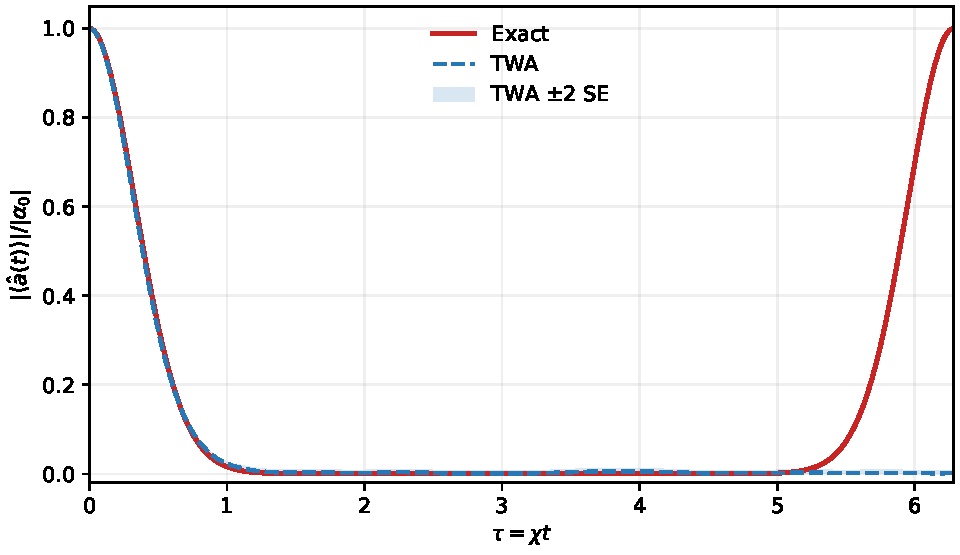
\includegraphics[width=0.82\textwidth]{figures/ch06/kerr_exact_vs_twa.pdf}
  \caption[Kerr 精确动力学与 TWA 的塌缩--回复对照]{相干态 Kerr 动力学的一阶相干性。黑线为 $N=9$ 的精确结果，蓝线为 $100000$ 条 TWA 轨迹的平均，阴影为 $\pm2$ 标准误。TWA 在所标早期窗口内再现塌缩，却不能在 $\tau=2\pi$ 重建量子回复；这张图检验的是该特定初态与观测量，不能据此宣称长时间 TWA 普遍有效。图由 \texttt{code/ch06\_kerr/kerr\_exact\_vs\_twa.py} 实际计算。}
  \label{fig:kerr-exact-vs-twa}
\end{figure}

在 $\tau\le0.25$ 的窗口内，归一化相干性最大绝对偏差为 $1.016\times10^{-2}$。在回复时刻，精确值为 $1$，TWA 为 $2.13\times10^{-3}$，其标准误为 $3.25\times10^{-3}$；即使计入 $4$ 个标准误，也与精确回复相差悬殊。正规排序粒子数的 TWA 初始估计为 $8.99958\pm0.00963$，解析值为 $9$；粒子数随后在每条 TWA 轨迹上保持。

这里的长时间差异不是轨迹数不足。继续增加轨迹数只会使 TWA 曲线更精确地趋近其连续经典系综极限，不会产生缺失的量子回复。完整指标保存在
\begin{center}
  \path{data/ch06/kerr_metrics.json}。
\end{center}

\section{塌缩不是热化}

Kerr 模型只有一个守恒占据和一个相位自由度，不具备在大量模式间重新分配能量的机制。$\qavg{\ha(t)}$ 的衰减是相位混合，不是热浴耗散，也不是多体碰撞热化。精确量子系统在 $2\pi/\chi$ 后回复，进一步证明早期衰减没有丢失信息。

在多模系统中，相位混合、动力学不稳定和真实的模式间散射可以同时发生。只观察一个相干因子下降，无法区分这些机制。需要结合模式占据、守恒量、可逆协议、关联函数和时间尺度判断。

\section{Weyl 修正为什么重要}

若错误地使用
\begin{equation}
  \ii\dot\alpha=\chi|\alpha|^2\alpha
\end{equation}
而忽略\cref{eq:kerr-twa-drift} 中的 $-1$，单条轨迹频率会整体偏移。对高占据 $N\gg1$，相对误差约为 $1/N$，短时间看似很小；但相位误差随时间积累，长时间比较会显著偏离。这个 $-1$ 来自哈密顿量的 Weyl 符号，不应通过经验调参补偿。

\begin{warningbox}
TWA 能准确描述塌缩，并不说明它也能描述随后的回复。判断有效性必须针对具体观测量和时间窗口，而不能只凭某个早期曲线吻合后把计算无限延长。
\end{warningbox}

\section{从 Kerr 模型学到的验证策略}

一个非线性 TWA 程序至少应通过以下检查：
\begin{enumerate}
  \item 在 $\chi=0$ 时退化为第5章的二次精确传播；
  \item 每条闭合轨迹保持 $|\alpha|^2$ 和 $H_W$；
  \item 相干态初始矩满足半量子修正；
  \item 在短时间窗口与\cref{eq:kerr-exact-mean} 收敛；
  \item 明确展示量子回复等已知失效现象，而不是隐藏长时间差异。
\end{enumerate}

\section*{本章小结}

Kerr 振子把 TWA 的能力边界压缩在一个可精确求解的模型中。非线性相位剪切造成的早期塌缩可以由初始 Wigner 涨落和经典漂移描述；离散量子谱造成的回复需要被截去的量子干涉。实际计算验证了早期吻合和长时间失效，并说明增加轨迹数不能修复方法误差。

\begin{exercises}
  \item 从 Fock 展开推导\cref{eq:kerr-exact-mean}。
  \item 由\cref{eq:kerr-weyl-hamiltonian} 推导\cref{eq:kerr-twa-drift}，解释频率中的 $-1$。
  \item 求精确相干性的半高宽随 $N$ 的标度。
  \item 修改程序比较 $N=1,9,100$，研究固定短时间窗口内的误差怎样随占据变化。
  \item 设计一次反转 $\chi\to-\chi$ 的回波协议，并比较精确动力学与数值积分误差。
\end{exercises}

\chapter{截断维格纳近似的推导}
\label{ch:twa-derivation}

\begin{learningobjectives}
完成本章后，读者应能：
\begin{enumerate}
  \item 从玻色 Hamiltonian 的 Wigner 方程识别一阶漂移和三阶量子项；
  \item 推导 Bose--Hubbard 型模型的 TWA 轨迹方程；
  \item 写出从初态抽样到正常排序观测量的算法；
  \item 说明高占据展开为何只提供有限时间、观测量相关的控制。
\end{enumerate}
\end{learningobjectives}

\section{从多模玻色 Hamiltonian 出发}

考虑 $M$ 个玻色模式，
\begin{equation}
  \Hhat=
  -\sum_{j,k}J_{jk}\had_j\ha_k
  +\sum_j\epsilon_j\had_j\ha_j
  +\sum_j\frac{U_j}{2}\had_j\had_j\ha_j\ha_j,
  \label{eq:bose-hubbard-general}
\end{equation}
其中 $J_{jk}=J_{kj}^*$，并约定对角跃迁项已并入 $\epsilon_j$。二次项的 Weyl 符号只产生常数和普通双线性项；局域四次项使用第2章结果。忽略与动力学无关的常数后，
\begin{equation}
  H_W=
  -\sum_{j,k}J_{jk}\alpha_j^*\alpha_k
  +\sum_j\epsilon_j\left(|\alpha_j|^2-\frac12\right)
  +\sum_j\frac{U_j}{2}
  \left(|\alpha_j|^4-2|\alpha_j|^2+\frac12\right).
  \label{eq:bose-hubbard-weyl}
\end{equation}

用 Bopp 规则作用于 von Neumann 方程，二次项只产生一阶导数，四次项产生一阶和三阶导数。相空间方程可以概括成
\begin{equation}
  \pder{W}{t}
  =-\sum_\mu\partial_\mu(A_\mu W)
  +\mathcal{L}^{(3)}W,
  \label{eq:wigner-first-third}
\end{equation}
其中 $\mu$ 遍历所有模式的实部和虚部，$\mathcal{L}^{(3)}$ 收集三阶导数。对于闭合、幺正的四次玻色 Hamiltonian，不会出现代表普通扩散的二阶项。

\section{截断操作}

TWA 定义为舍弃\cref{eq:wigner-first-third} 中的 $\mathcal{L}^{(3)}$：
\begin{equation}
  \pder{W_{\mathrm{TWA}}}{t}
  =-\sum_\mu\partial_\mu(A_\mu W_{\mathrm{TWA}}).
  \label{eq:twa-liouville}
\end{equation}
这是 Liouville 型连续性方程，可由确定性特征线求解。复振幅方程为
\begin{equation}
  \ii\hbar\dot\alpha_j
  =\pder{H_W}{\alpha_j^*}
  =-\sum_kJ_{jk}\alpha_k
  +\left[\epsilon_j+U_j(|\alpha_j|^2-1)\right]\alpha_j.
  \label{eq:twa-bose-hubbard-drift}
\end{equation}
$-1$ 是每个局域模式的 Weyl 修正。若占据很大，它相对于 $|\alpha_j|^2$ 较小；若某些模式接近真空，则不能仅凭“总粒子数很大”忽略它。

\begin{derivationbox}
把单模相互作用的 Weyl 符号写成
\[
  H_{W,\mathrm{int}}=\frac{U}{2}
  (\alpha^{*2}\alpha^2-2\alpha^*\alpha+1/2).
\]
将 $\alpha$ 和 $\alpha^*$ 当作独立变量，便有
\[
  \pder{H_{W,\mathrm{int}}}{\alpha^*}
  =U(|\alpha|^2-1)\alpha.
\]
这一步同时检查了非线性系数和排序修正。
\end{derivationbox}

\section{TWA 算法}

对给定 $\rhohat_0,\Hhat,\Ohat$，可执行的算法为：
\begin{enumerate}
  \item 选择有限模式或空间网格，并固定对易关系和归一化；
  \item 求 $W_0(\bm\alpha,\bm\alpha^*)$，或至少求目标近似所需的均值与协方差；
  \item 生成 $N_s$ 个初值 $\bm\alpha^{(s)}(0)$；
  \item 对每个样本独立积分\cref{eq:twa-bose-hubbard-drift}；
  \item 由 $O_W[\bm\alpha^{(s)}(t)]$ 计算样本均值和标准误差；
  \item 改变轨迹数、时间步长、模式截止和系统尺寸，并与独立基准比较。
\end{enumerate}
步骤2和步骤5都依赖算符排序。只要把真空噪声加到 GPE 初值却省略 Weyl 漂移或观测量修正，就不是自洽的 TWA。

\begin{numericalbox}
闭合系统的轨迹在给定初值后是确定性的，最适合并行计算。可复现记录至少包括随机种子生成规则、轨迹数、积分器、容差、模式基底、截止和所有 Weyl 修正。不要只保存系综平均曲线；抽查单轨迹守恒量有助于发现积分错误。
\end{numericalbox}

\section{高占据展开的含义}

若典型模式占据为 $N\gg1$，可写 $\alpha=\sqrt{N}\,\psi$，并在保持平均场非线性能标有限的方式下缩放相互作用。此时一阶漂移给出领先的经典场动力学，高阶 Moyal 导数在形式上受到 $1/N$ 幂次抑制\cite{Polkovnikov2010}。这解释了 TWA 在高占据、有限时间条件下常有效。

但这一计数不是无条件误差界。至少有四个例外：
\begin{enumerate}
  \item 动力学把粒子输运到大量低占据模式；
  \item 不稳定流指数放大初始和截断误差；
  \item 长时间形成细相空间干涉结构；
  \item 目标观测量本身对高阶关联或稀有尾部敏感。
\end{enumerate}
因此，有效性应写成“在指定参数、观测量和时间窗口内通过基准”，而不是“因为总粒子数大所以有效”。

\section{TWA 保留了哪些量子信息}

TWA 保留：
\begin{itemize}
  \item 初态 Wigner 分布中的真空、热和压缩涨落；
  \item 模间协方差和反常关联；
  \item Weyl Hamiltonian 中的排序修正；
  \item 由非线性经典流把初始涨落转换成观测量涨落的过程。
\end{itemize}
它通常不保留由高阶 Moyal 项生成的完整量子干涉、负值细结构、晚时回复和所有高阶纠缠信息。Kerr 例子显示，初期量子涨落的影响可以正确，晚时离散谱干涉仍然缺失。

“量子力学只存在于初始条件中”因而不是严格表述。更准确地说，TWA 把动力学近似为 Weyl Hamiltonian 产生的经典漂移，同时通过初态分布和观测量排序保留领先量子修正；被截去的是一类真正的动力学量子修正\cite{Steel1998,Sinatra2002}。

\section{守恒量与截断误差}

若\cref{eq:twa-bose-hubbard-drift} 由时间无关的 $H_W$ 生成，连续时间轨迹保持 $H_W$。若 Hamiltonian 具有全局 $U(1)$ 对称性，还保持
\begin{equation}
  N_W=\sum_j(|\alpha_j|^2-1/2).
\end{equation}
数值程序明显破坏这些守恒量意味着积分误差，但守恒量保持并不证明 TWA 等于精确量子动力学。Kerr TWA 在回复时刻仍精确守恒粒子数和 $H_W$，却给出错误相干性。

\begin{warningbox}
轨迹守恒检查是必要条件，不是方法正确性的充分条件。系统误差需要精确小系统、Bogoliubov 极限、短时间展开或另一种受控方法来估计。
\end{warningbox}

\section*{本章小结}

四次玻色 Hamiltonian 的精确 Wigner 方程含一阶和三阶导数。TWA 舍弃三阶项，得到由 Weyl Hamiltonian 驱动的确定性经典场轨迹。初态抽样、漂移中的排序修正和观测量估计器必须使用同一约定。高占据提供形式上的半经典展开，但实际可信度仍取决于模式占据、时间、稳定性和观测量。

\begin{exercises}
  \item 从\cref{eq:bose-hubbard-weyl} 推导多模漂移\cref{eq:twa-bose-hubbard-drift}。
  \item 证明实对称跃迁矩阵下 $\sum_j|\alpha_j|^2$ 沿 TWA 轨迹守恒。
  \item 对两体非局域相互作用 $V_{jk}\hat n_j\hat n_k$，讨论 $j=k$ 与 $j\neq k$ 的 Weyl 修正差别。
  \item 解释为什么增加 $N_s$ 可以减小抽样误差，却不改变三阶导数被舍弃这一事实。
  \item 为一个含低占据散射模的模型设计至少两个 TWA 失效诊断。
\end{exercises}

\chapter{Bose--Hubbard 二聚体}
\label{ch:dimer}

\begin{learningobjectives}
完成本章后，读者应能：
\begin{enumerate}
  \item 从两模 Bose--Hubbard Hamiltonian 推导精确矩阵表示和 TWA 方程；
  \item 用数差与相对相位解释 Rabi 振荡、相位扩散和非线性自俘获；
  \item 在完全相同的初态与观测量下比较精确演化、平均场和 TWA；
  \item 检查 Fock 截断、Monte Carlo 误差和轨迹守恒量。
\end{enumerate}
\end{learningobjectives}

\section{连接单模与量子场的最小模型}

两模 Bose--Hubbard Hamiltonian 为
\begin{equation}
  \Hhat=-J(\had_L\ha_R+\had_R\ha_L)
  +\frac{U}{2}\sum_{\sigma=L,R}
  \had_\sigma\had_\sigma\ha_\sigma\ha_\sigma.
  \label{eq:dimer-hamiltonian}
\end{equation}
$J$ 与 $U$ 均为能量。它可以描述双阱、两个内部态的单空间模近似，或完整场论的最低两模截断。总粒子数
\begin{equation}
  \hat N=\hat n_L+\hat n_R
\end{equation}
严格守恒，但左右数差
\begin{equation}
  \hat Z=\hat n_L-\hat n_R
\end{equation}
会因隧穿而振荡。

当 $U=0$ 时，每个粒子作线性 Rabi 振荡；当 $J=0$ 时，各模式的粒子数固定，而不同数分量因相互作用积累不同相位；两者竞争时出现振幅依赖的非线性 Josephson 动力学。这个模型既可在有限 Fock 空间精确求解，也具有非平凡 TWA，因此适合系统基准。

\section{固定粒子数表象}

在固定总数 $N$ 的子空间中，基底可取
\begin{equation}
  \ket{n,N-n},\qquad n=0,1,\ldots,N.
\end{equation}
对角矩阵元为
\begin{equation}
  \mel{n,N-n}{\Hhat}{n,N-n}
  =\frac{U}{2}\left[n(n-1)+(N-n)(N-n-1)\right],
\end{equation}
相邻基矢由隧穿连接：
\begin{equation}
  \mel{n+1,N-n-1}{\Hhat}{n,N-n}
  =-J\sqrt{(n+1)(N-n)}.
  \label{eq:dimer-matrix-element}
\end{equation}
因此每个固定 $N$ 块只有 $N+1$ 维。若初态是两个相干态的直积，则总数不是固定值；精确计算需要同时包含多个 $N$ 块，或在每个模式上设置足够高的 Fock 截断。

\section{Weyl Hamiltonian 与 TWA 方程}

\cref{eq:dimer-hamiltonian} 的 Weyl 符号在略去常数后为
\begin{equation}
  H_W=-J(\alpha_L^*\alpha_R+\alpha_R^*\alpha_L)
  +\frac{U}{2}\sum_{\sigma=L,R}
  \left(|\alpha_\sigma|^4-2|\alpha_\sigma|^2\right).
  \label{eq:dimer-weyl}
\end{equation}
TWA 轨迹满足
\begin{align}
  \ii\hbar\dot\alpha_L
  &=-J\alpha_R+U(|\alpha_L|^2-1)\alpha_L,\\
  \ii\hbar\dot\alpha_R
  &=-J\alpha_L+U(|\alpha_R|^2-1)\alpha_R.
  \label{eq:dimer-twa}
\end{align}
每条连续轨迹保持 $|\alpha_L|^2+|\alpha_R|^2$ 与 $H_W$。正常排序总数估计为
\begin{equation}
  \qavg{\hat N}
  =\ensavg{|\alpha_L|^2+|\alpha_R|^2-1},
  \label{eq:dimer-total-estimator}
\end{equation}
而数差中的两个半量子互相抵消：
\begin{equation}
  \qavg{\hat Z}
  =\ensavg{|\alpha_L|^2-|\alpha_R|^2}.
\end{equation}

\section{数差与相对相位}

在高占据区写
\begin{equation}
  \alpha_L=\sqrt{\frac{N_c}{2}(1+z)}\,\ee^{-\ii\phi/2},
  \qquad
  \alpha_R=\sqrt{\frac{N_c}{2}(1-z)}\,\ee^{\ii\phi/2}.
\end{equation}
$z$ 是归一化数差，$\phi$ 是相对相位，$N_c=|\alpha_L|^2+|\alpha_R|^2$ 沿轨迹守恒。忽略与 $z,\phi$ 无关的常数后，经典 Hamiltonian 具有结构
\begin{equation}
  H_{\mathrm{rel}}
  =\frac{UN_c^2}{4}z^2
  -JN_c\sqrt{1-z^2}\cos\phi.
  \label{eq:josephson-classical-hamiltonian}
\end{equation}
数差和相对相位构成共轭变量。初始数差涨落造成不同轨迹具有不同的相位速度，这是相位扩散的直接来源。若相互作用能相对隧穿足够大，经典相图出现分离曲线和自俘获轨道；但量子隧穿、有限 $N$ 与初态宽度会使锐利的经典边界变成有限尺寸交叉。

\section{精确计算与 TWA 的同协议比较}

本章数值实验取 $\hbar=J=1$、$U=0.15$，初态为
\begin{equation}
  \ket{\psi_0}=\ket{\alpha_L=\sqrt8}\otimes\ket{\alpha_R=0}.
  \label{eq:dimer-coherent-initial}
\end{equation}
这是一项有意选择的基准：相干态 Wigner 函数可精确正抽样，因而比较不含固定粒子数态近似抽样的额外误差。代价是总粒子数服从 Poisson 分布；本结果不能直接解释为固定 $N=8$ 的实验。

精确演化在每模 $n=0,\ldots,23$ 的截断 Fock 空间中计算。截断前保留的初态范数为 $0.9999963$，随后重新归一化。TWA 使用 $20000$ 条相干态 Wigner 轨迹和四阶 Runge--Kutta 积分。比较量为
\begin{equation}
  z(t)=\frac{\qavg{\hat n_L}-\qavg{\hat n_R}}
  {\qavg{\hat n_L}+\qavg{\hat n_R}}.
  \label{eq:dimer-imbalance}
\end{equation}

\begin{figure}[htbp]
  \centering
  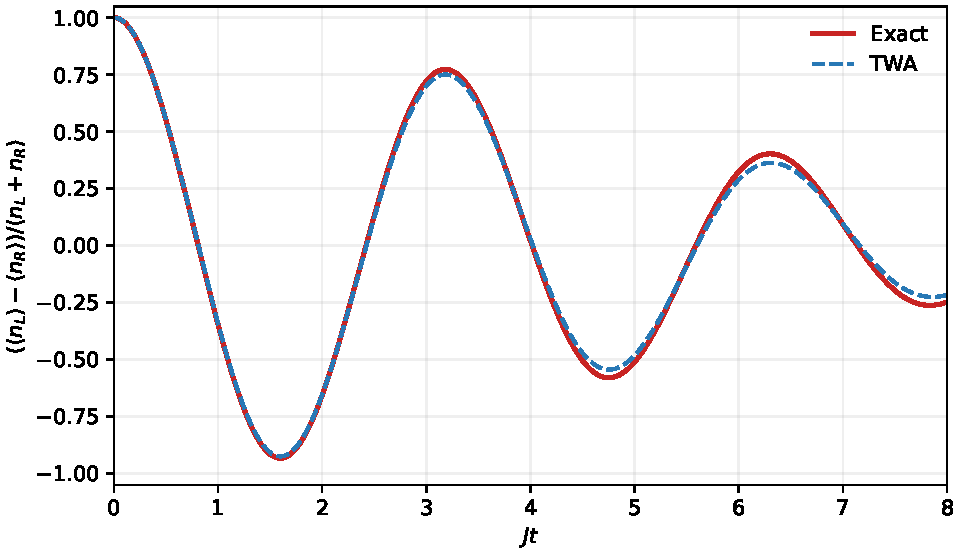
\includegraphics[width=0.82\textwidth]{figures/ch08/dimer_exact_vs_twa.pdf}
  \caption{两模 Bose--Hubbard 模型的归一化数差。红色实线为截断 Fock 空间的量子演化，蓝色虚线为 TWA。参数、初态和观测量在两种计算中完全一致。图由 \texttt{code/ch08\_dimer/dimer\_exact\_vs\_twa.py} 生成。}
  \label{fig:dimer-exact-vs-twa}
\end{figure}

在 $t\le2/J$ 的窗口内，最大数差误差为 $8.03\times10^{-3}$；整个 $0\le Jt\le8$ 窗口的均方根误差为 $2.13\times10^{-2}$。TWA 正常排序总数的绝对漂移为 $2.45\times10^{-7}$。这些结果说明在本参数与观测量下，TWA 在所展示窗口内表现良好，但不能外推为更强相互作用、更低占据或任意长时间下的普遍精度。

完整指标保存在
\begin{center}
  \path{data/ch08/dimer_metrics.json}。
\end{center}

\begin{numericalbox}
公平基准必须保持四项相同：初态密度算符、Hamiltonian 参数、目标观测量和时间采样。用固定 $N$ 精确解去比较相干态 TWA 抽样，会把初态差别误记为动力学误差。
\end{numericalbox}

\section{三个互补误差检查}

\subsection{Fock 截断}

增大每模最大占据，检查初态保留范数和观测量曲线。只报告矩阵维数不够；若初态在截断边界仍有显著概率，时间演化会被人工反射。

\subsection{轨迹与积分}

分别增大轨迹数和减小时间步长。前者改变统计噪声，后者改变单轨迹守恒误差；两种收敛不能用同一条曲线替代。

\subsection{初态模型}

固定总粒子数的 SU(2) 相干态、两个 Glauber 相干态直积和数压缩态具有不同的数差及总数涨落。若研究相位扩散，初态模型通常比平均密度的微小差异更重要。

\begin{warningbox}
二聚体中的系综相干性下降可以来自可逆相位混合。它不是证明环境耗散、不可逆碰撞或热化的充分证据。必须结合回波、频谱和更多模式的能量再分配进行判断。
\end{warningbox}

\section*{本章小结}

Bose--Hubbard 二聚体把单模非线性推广为具有粒子交换的最小多模系统。精确 Fock 计算与 TWA 使用相同相干初态后，在本章参数的有限时间窗口内高度一致。模型同时说明数差与相位的共轭关系、Weyl 半量子修正、固定数与相干态的差别，以及公平基准必须控制的截断和抽样误差。

\begin{exercises}
  \item 推导固定 $N$ 基底中的矩阵元\cref{eq:dimer-matrix-element}。
  \item 从\cref{eq:dimer-weyl} 推导 TWA 方程\cref{eq:dimer-twa}。
  \item 在 $U=0$ 时求初态 $\ket{N,0}$ 的精确数差振荡。
  \item 修改配套程序，把每模 Fock 截断依次设为 16、20、24、28，比较保留范数与曲线误差。
  \item 设计固定总粒子数初态与相干直积态的公平比较，并列出需要匹配和不应匹配的统计量。
\end{exercises}

\chapter{TWA 的有效范围与失效模式}
\label{ch:validity}

\begin{learningobjectives}
完成本章后，读者应能：
\begin{enumerate}
  \item 把 TWA 误差分解为状态表示、动力学截断、数值离散和抽样误差；
  \item 根据占据、模式数、不稳定性、观测量和时间窗口评估风险；
  \item 设计模式截止、轨迹数和独立方法的验证矩阵；
  \item 避免用经典场晚时热化替代量子热化结论。
\end{enumerate}
\end{learningobjectives}

\section{有效性不是一个布尔变量}

“TWA 对这个模型有效吗”缺少三个必要限定：对哪个初态、哪个观测量、哪个时间窗口。第5章的二次系统对任意时间和任意初态分布都有精确 Wigner 漂移；第6章 Kerr 模型在早期相干性上准确，却完全错过回复；第8章二聚体在指定参数和数差观测量上通过有限时间基准。这些例子说明，有效性必须写成带条件的命题。

一项 TWA 结果至少包含四层近似：
\begin{enumerate}
  \item \textbf{状态表示}：初态 Wigner 函数是否精确可抽样，或只匹配了有限矩；
  \item \textbf{动力学截断}：高阶 Moyal 导数是否在目标窗口内可忽略；
  \item \textbf{数值表示}：有限模式、网格、时间步长和浮点误差；
  \item \textbf{统计估计}：有限轨迹和相关样本导致的不确定度。
\end{enumerate}
只有第四层误差必然按 $N_s^{-1/2}$ 缩小。增加轨迹数对前三层没有系统修复作用。

\section{支持 TWA 的条件}

\subsection{相关模式高占据}

半经典展开通常要求对动力学和观测量重要的模式具有大于单位量级的占据。这里的“相关模式”不是任意选定的粗网格模式；若非线性散射不断把半量子噪声送入低占据高能模，总粒子数很大仍不足以保证可靠。经典场研究常用“粒子数显著大于保留模式数”作为必要的经验条件之一\cite{Sinatra2002,Blakie2008}。

\subsection{有限时间和光滑相空间结构}

初始 Wigner 分布在相空间尺度上光滑，且经典流尚未形成细密折叠时，高阶导数较不重要。混沌或动力学不稳定可以指数放大微小结构，使有效时间明显短于平稳系统。不存在只依赖 $N$、适用于所有模型和观测量的统一失效时间公式。

\subsection{低阶、粗粒化观测量}

密度、低阶等时关联和大尺度结构因子通常更适合 TWA。Wigner 负值、高阶尾部、量子回波和精确回复对干涉结构更敏感；即使平均占据很高，相关计算也可能失败。

\section{模式截止与半量子噪声}

每个保留玻色模式在真空中贡献半个对称排序量子。若保留 $M$ 个模式，初始经典场中含有数量级为 $M/2$ 的虚拟占据。正确的等时估计器会减去对应排序项，但非线性轨迹仍会让这些高能噪声参与散射。

因此，细化网格会同时做两件事：提高空间分辨率，并加入更多真空噪声模式。若结果随截止显著变化，不能简单选择“最细网格”作为答案。需要寻找物理观测量对截止稳定的窗口，或采用正规化、投影经典场和更合适的量子方法。针对凝聚气体的分析表明，晚时经典场可能趋向与目标量子温度不同的经典平衡，从而产生伪阻尼\cite{Sinatra2002}。

\begin{warningbox}
网格收敛不是单调的“越细越好”。在 TWA 中，改变网格还改变了真空噪声总量和可发生散射的高能通道；必须同时记录模式数、粒子数和截止能量。
\end{warningbox}

\section{长时间热化的特别风险}

闭合量子系统的幺正演化微观可逆。局域观测量可以因去相位和模式混合趋于稳态，但“不可逆”通常是粗粒化意义。TWA 轨迹同样是可逆 Hamilton 流，其系综可以相空间混合；与此同时，经典非线性场可能向 Rayleigh--Jeans 型分布演化。后者依赖紫外截止，不能自动等同于 Bose--Einstein 量子热平衡。

声称“完全热化”至少应提供：
\begin{enumerate}
  \item 能量、粒子数和其他守恒量的闭合账目；
  \item 多个初态在相同守恒量下趋于同一粗粒化结果；
  \item 模式分布与候选统计系综的定量比较；
  \item 模式截止和网格变化下的稳定性；
  \item 在可重叠区与动理学、精确小系统或其他量子方法比较；
  \item 对预热化、积分性和有限尺寸回复的排除或限定。
\end{enumerate}
仅观察相干因子下降或单个动量峰变宽，不足以满足这些条件。

\section{验证矩阵}

推荐把验证设计成互补矩阵：
\begin{center}
\begin{tabularx}{\textwidth}{p{0.20\textwidth}X X}
\toprule
检查 & 能证明什么 & 不能证明什么 \\
\midrule
增加轨迹数 & Monte Carlo 均值和误差条稳定 & 动力学截断正确 \\
减小时间步长 & 积分器收敛、守恒误差下降 & 连续 TWA 接近量子解 \\
改变网格/截止 & 结果对数值表示稳定 & 所有未保留模式都不重要 \\
二次极限 & 抽样、漂移和排序实现一致 & 非线性长时间可靠 \\
精确小系统 & 指定参数和观测量的总误差 & 热力学极限必然相同 \\
Bogoliubov 极限 & 弱涨落线性响应正确 & 强非线性晚时正确 \\
\bottomrule
\end{tabularx}
\end{center}

最有价值的验证不是重复同一类收敛，而是让不同误差源具有不同响应。例如轨迹数变化只影响统计噪声，时间步长变化影响守恒漂移，Fock 截断影响精确基准，系统尺寸变化影响有限尺寸物理。

\section{按风险选择替代方法}

若初态具有强 Wigner 负值，可考虑 positive-P、离散 Wigner 或直接 Fock/张量网络表示；若系统是一维低纠缠短程模型，MPS 往往比连续场 TWA 更受控；若占据低但模式数少，精确对角化更直接；若关注弱耦合长时间碰撞，量子 Boltzmann 或 Keldysh 动理学可能比盲目延长 TWA 更合适。开放系统则需保留主方程产生的扩散和噪声。

方法选择不应以“哪个能跑到更大尺寸”为唯一标准。还要问目标结论依赖哪类量子信息，以及候选方法是否保存这些信息。

\section{结论强度与证据强度}

建议采用以下层级：
\begin{enumerate}
  \item \textbf{数值观察}：在给定离散化和轨迹数下出现某趋势；
  \item \textbf{TWA 稳健结果}：趋势通过抽样、步长与截止检查；
  \item \textbf{受基准支持的量子结论}：在重叠区与独立量子方法一致；
  \item \textbf{热力学或普适结论}：还需系统尺寸标度、序参量定义和理论论证。
\end{enumerate}
写作时应把结论停在证据实际达到的层级。第17章讨论超固态时将严格使用这一规则。

\begin{chaptercheck}
在运行大规模轨迹前先写下失效判据：哪些模式可能变成低占据，哪个观测量最敏感，何时与基准比较，怎样改变截止。若只有“轨迹数足够多”这一项，验证计划尚未完成。
\end{chaptercheck}

\section*{本章小结}

TWA 的有效性依赖初态、相关模式占据、动力学稳定性、观测量和时间窗口。半量子噪声使模式截止成为物理与数值耦合的问题，尤其限制晚时热化解释。可靠结论需要把抽样、积分、表示和方法误差分别检验，并用与结论强度相匹配的独立证据支撑。

\begin{exercises}
  \item 为第6章 Kerr 例子填写本章验证矩阵，并指出哪个检查能暴露回复失败。
  \item 设一维网格长度固定、格点数加倍，计算真空半量子总数怎样变化。
  \item 设计一个区分相位混合与能量热化的数值协议。
  \item 对一个含 $10^5$ 个粒子和 $10^4$ 个模式的模拟，讨论总平均占据为何不足以描述占据分布风险。
  \item 为“系统在热力学极限中形成长程密度序”列出至少四类独立证据。
\end{exercises}


\part{玻色量子场与数值实现}
\chapter{从玻色模式到离散量子场}
\label{ch:bose-field}

\begin{learningobjectives}
完成本章后，读者应能：
\begin{enumerate}
  \item 从连续玻色场构造保持正则对易关系的有限模式表示；
  \item 推导格点场的半量子修正及其对粒子数和相互作用漂移的影响；
  \item 区分物理场、数值场、投影场与裸格点变量；
  \item 把模式截止看作模型定义的一部分，而不只是计算精度旋钮。
\end{enumerate}
\end{learningobjectives}

\section{连续场只是起点}

一分量玻色场满足
\begin{equation}
  \comm{\hpsi(x)}{\hpsid(x')}=\delta(x-x'),
  \qquad
  \comm{\hpsi(x)}{\hpsi(x')}=0 .
  \label{eq:continuous-commutator}
\end{equation}
以一维接触相互作用为例，二次量子化哈密顿量写成
\begin{equation}
  \Hhat=\int\dd x\,\hpsid(x)h_0\hpsi(x)
  +\frac{g}{2}\int\dd x\,\hpsid(x)^2\hpsi(x)^2,
  \qquad
  h_0=-\frac{\hbar^2}{2m}\partial_x^2+V(x).
  \label{eq:continuum-bose-hamiltonian}
\end{equation}
这里的 $g$ 是与维数和降维方案相匹配的有效耦合常数。三维散射长度不能在一维代码中未经降维就直接充当 $g$。
弱相互作用凝聚气体的场论背景可参见\cite{Dalfovo1999}；投影经典场与
functional Wigner 的截止、投影核和半量子处理可与
\cite{Blakie2008,Opanchuk2013}交叉核对。

计算机不能直接保存无穷多个场自由度。选择有限模式并不是无害的排版步骤：它规定了哪些量子涨落被保留、每个模式的半量子噪声进入何处，以及接触相互作用的裸参数应如何解释。因此，本章先固定有限维模型，再讨论其 TWA。

\section{有限模式投影}

取一组正交单粒子模式 $\{\phi_n(x)\}_{n\in\mathcal C}$，保留集合记作 $\mathcal C$：
\begin{equation}
  \hpsi_{\mathcal C}(x)=\sum_{n\in\mathcal C}\phi_n(x)\ha_n,
  \qquad
  \comm{\ha_n}{\had_m}=\delta_{nm}.
  \label{eq:projected-field}
\end{equation}
投影场不再满足完整 Dirac delta，而满足
\begin{equation}
  \comm{\hpsi_{\mathcal C}(x)}{\hpsid_{\mathcal C}(x')}
  =\delta_{\mathcal C}(x,x'),
  \qquad
  \delta_{\mathcal C}(x,x')
  =\sum_{n\in\mathcal C}\phi_n(x)\phi_n^*(x').
  \label{eq:projected-delta}
\end{equation}
$\delta_{\mathcal C}(x,x)$ 是单位长度内的保留模式密度。它将在排序修正中取代形式上发散的 $\delta(0)$。

模式振幅 $\alpha_n$ 是无量纲变量，经典投影场定义为
\begin{equation}
  \psi_{\mathcal C}(x)=\sum_{n\in\mathcal C}\phi_n(x)\alpha_n .
  \label{eq:classical-projected-field}
\end{equation}
真空对每个 $\alpha_n$ 贡献 $\ensavg{|\alpha_n|^2}=1/2$，所以
\begin{equation}
  \ensavg{|\psi_{\mathcal C}(x)|^2}_{\rm vac}
  =\frac{1}{2}\delta_{\mathcal C}(x,x).
  \label{eq:projected-vacuum-density}
\end{equation}
这不是实际粒子密度，而是对称排序的半量子基线。

\section{均匀格点与变量归一化}

连续场是算符值分布，未经投影的 ``$\hpsi(x_j)$'' 不能直接乘以
$\sqrt{\Delta x}$ 就变成严格的正则模式。以下等式应理解为一个有限维
Fourier--DVR 构造。具体地，在长度 $L$ 的周期区间保留 $M$ 个平面波，取
$M$ 个等距格点 $x_j$ 和 $\Delta x=L/M$，并定义基数函数
\begin{equation}
  \chi_j(x)=\sqrt{\Delta x}\,\delta_{\mathcal C}(x,x_j),
  \qquad
  \int\dd x\,\chi_j^*(x)\chi_k(x)=\delta_{jk}.
  \label{eq:grid-cardinal-mode}
\end{equation}
相应的格点模式算符才是
\begin{equation}
  \ha_j=\int\dd x\,\chi_j^*(x)\hpsi_{\mathcal C}(x)
  =\sqrt{\Delta x}\,\hpsi_{\mathcal C}(x_j),
  \qquad
  \comm{\ha_j}{\had_k}=\delta_{jk}.
  \label{eq:grid-mode-definition}
\end{equation}
最后一个等号只对这里的带限投影场成立；它不是对完整连续场的逐点
采样恒等式。若使用有限体积胞元模式，则应改为对胞元积分，下面的
$\psi_j$ 相应代表胞元平均而非严格点值。

令 $\alpha_j$ 是 $\ha_j$ 的 Wigner 振幅，并定义
\begin{equation}
  \psi_j=\frac{\alpha_j}{\sqrt{\Delta x}}.
  \label{eq:grid-field-normalization}
\end{equation}
$\alpha_j$ 无量纲，而 $\psi_j$ 的量纲为长度$^{-1/2}$。二者混用会令噪声、耦合常数和粒子数同时错一个 $\Delta x$ 因子。

格点真空抽样可写成
\begin{equation}
  \alpha_j^{\rm vac}=\frac{\xi_{1j}+\ii\xi_{2j}}{2},
  \qquad \xi_{1j},\xi_{2j}\sim\mathcal N(0,1),
  \label{eq:grid-vacuum-sampling}
\end{equation}
因而 $\ensavg{|\alpha_j^{\rm vac}|^2}=1/2$，以及
\begin{equation}
  \ensavg{|\psi_j^{\rm vac}|^2}=\frac{1}{2\Delta x}.
  \label{eq:grid-vacuum-density}
\end{equation}
格点密度的正规排序估计器是
\begin{equation}
  \qavg{\hpsid(x_j)\hpsi(x_j)}
  \approx \ensavg{|\psi_j|^2}-\frac{1}{2\Delta x}.
  \label{eq:grid-density-estimator}
\end{equation}
相应的总粒子数为
\begin{equation}
  N=\Delta x\sum_{j=0}^{M-1}\ensavg{|\psi_j|^2}-\frac{M}{2}
  =\sum_j\ensavg{|\alpha_j|^2}-\frac{M}{2}.
  \label{eq:grid-total-number}
\end{equation}

\begin{warningbox}
若代码输出 $\mathcal N_{\mathrm{sym}}=\Delta x\sum_j|\psi_j|^2$ 而没有减去
$M/2$，它输出的是原始对称范数，不是粒子数 Weyl 符号 $N_W$。这个差异在
$N\gg M$ 时可能相对很小，却会系统污染耗尽量、低密度尾部和模式占据。
\end{warningbox}

\section{离散哈密顿量与 Weyl 漂移}

在上述 Fourier--DVR 的等距求积约定下，连续相互作用的离散模型为
\begin{equation}
  \Hhat_{\rm int}=\frac{g}{2\Delta x}\sum_j\had_j{}^2\ha_j^2.
  \label{eq:grid-interaction-hamiltonian}
\end{equation}
因此单格点等效 Bose--Hubbard 参数为 $U=g/\Delta x$。利用第7章的单模对应，省略不影响漂移的常数后，其 Weyl 符号是
\begin{equation}
  H_{{\rm int},W}
  =\frac{g\Delta x}{2}\sum_j
  \left(
  |\psi_j|^4-\frac{2}{\Delta x}|\psi_j|^2
  +\frac{1}{2\Delta x^2}
  \right).
  \label{eq:grid-interaction-weyl}
\end{equation}
取 Hamilton 方程得到格点 TWA 漂移
\begin{equation}
  \ii\hbar\frac{\dd\psi_j}{\dd t}
  =\sum_k (h_0)_{jk}\psi_k
  +g\left(|\psi_j|^2-\frac{1}{\Delta x}\right)\psi_j.
  \label{eq:grid-twa-equation}
\end{equation}
这里的 $1/\Delta x$ 是相互作用漂移的 Weyl 修正；密度估计器中的修正则是 $1/(2\Delta x)$。二者来自不同次数的算符乘积，不能因为都与“半量子”有关就互相替换。

在一般投影基中，局域表达的对应结构是
\begin{equation}
  \ii\hbar\partial_t\psi_{\mathcal C}(x)
  =\mathcal P_{\mathcal C}\!\left\{
  \left[h_0+g\left(|\psi_{\mathcal C}(x)|^2
  -\delta_{\mathcal C}(x,x)\right)\right]
  \psi_{\mathcal C}(x)\right\},
  \label{eq:projected-twa-equation}
\end{equation}
其中 $\mathcal P_{\mathcal C}$ 把非线性项投回保留子空间。若省略该投影，非线性乘积会生成截止之外的模式，并通过混叠折回低波数区。

\section{动能离散：有限差分还是谱方法}

二阶中心差分给出
\begin{equation}
  -\partial_x^2\psi_j\approx
  -\frac{\psi_{j+1}-2\psi_j+\psi_{j-1}}{\Delta x^2},
  \label{eq:finite-difference-laplacian}
\end{equation}
其优点是边界条件直观、矩阵稀疏；缺点是高波数色散偏离连续谱。周期体系常采用 Fourier 谱方法：先变换到 $k$ 空间，再把动能乘子取为 $\hbar^2k^2/(2m)$。谱方法对光滑周期场具有高精度，但隐含周期边界，并要求显式处理非线性混叠。

两种离散并不定义同一个有限维模型。比较结果时应报告：区间长度、边界条件、格点数、动能算符、最大波数、相互作用参数的离散约定，以及是否投影非线性项。

\section{截止、重整化与连续极限}

保持 $L$ 固定并令 $M\to\infty$ 时，半量子总数 $M/2$ 发散，$\delta_{\mathcal C}(x,x)$ 也随截止增大。正规排序估计器可以在初时抵消真空基线，却不能阻止非线性轨迹让紫外噪声参与散射。因此，裸接触相互作用的 TWA 不应通过盲目加密网格来宣称已经取得连续极限。

实践中应区分三种问题：
\begin{enumerate}
  \item \textbf{数值收敛}：固定有限模式模型，减小时间步长和积分误差；
  \item \textbf{表示稳定}：在一组物理合理的截止内改变 $M$，检查目标观测量；
  \item \textbf{理论重整化}：若要求真正的截止无关连续预测，重新匹配耦合常数或采用保留量子紫外行为的方法。
\end{enumerate}
第1项通过并不自动证明第2、3项。

``重新匹配耦合常数'' 必须落实为一个可复现的两体协议，而不能靠观察
多体结果后调参。对每个候选截止 $\Lambda$，先选定一个物理输入量---例如
有限体积最低两体能级、一维低能散射相移或三维散射长度---再用同一动能
离散和边界条件求解两体问题，调节裸参数 $g_{\rm bare}(\Lambda)$ 直至该输入量
复现。随后保持这个匹配规则不变，预测另一个两体量作为交叉检查，最后才
进入多体 TWA。准一维模型还须先由横向束缚得到有效 $g_{1\rm D}$，并保证
能量与截止均未越过降维的适用区。这个两体匹配只能控制哈密顿量参数
的截止依赖；它不能消除 TWA 半量子在非线性长时间演化中的紫外散射。

\section{实现前的量纲检查}

选取长度 $x_0$、能量 $E_0=\hbar^2/(2mx_0^2)$ 和时间 $t_0=\hbar/E_0$ 后，可定义
\begin{equation}
  \tilde x=x/x_0,
  \qquad
  \tilde t=t/t_0,
  \qquad
  \tilde\psi=\sqrt{x_0}\,\psi,
  \qquad
  \tilde g=g/(E_0x_0).
\end{equation}
无量纲粒子数仍为 $N=\int\dd\tilde x\,|\tilde\psi|^2$。建议代码只传播无量纲变量，并在输入与输出边界统一转换；不要让带单位的 $g$、无量纲 $\Delta x$ 和 SI 制的时间混在同一个右端函数中。

\begin{chaptercheck}
对真空运行一次零相互作用测试。程序应得到：每格点 $\ensavg{|\alpha_j|^2}=1/2$，对称排序总范数约为 $M/2$，而式\eqref{eq:grid-total-number}给出的正规排序粒子数在统计误差内为零。若三项不能同时成立，先修复归一化，再进行任何动力学模拟。
\end{chaptercheck}

\section*{本章小结}

连续玻色场必须先投影到有限模式子空间，才成为可计算且定义良好的相空间模型。格点变量 $\alpha_j$ 与物理场 $\psi_j$ 相差 $\sqrt{\Delta x}$；真空密度基线、正规排序密度修正和相互作用 Weyl 漂移分别由这一归一化决定。模式截止同时控制空间分辨率和半量子噪声，因而是模型和验证协议的一部分。

\begin{exercises}
  \item 从式\eqref{eq:grid-interaction-hamiltonian}的单模 Weyl 符号推导式\eqref{eq:grid-interaction-weyl}和\eqref{eq:grid-twa-equation}。
  \item 对长度固定的周期网格，把格点数从 $M$ 增至 $2M$，比较 $\Delta x$、真空场方差、半量子总数和最大波数的变化。
  \item 证明式\eqref{eq:projected-vacuum-density}，并在平面波基中计算 $\delta_{\mathcal C}(x,x)$。
  \item 写出周期边界下中心差分 Laplace 算符的本征值，并与连续 $k^2$ 色散比较。
  \item 设计一个能够分别检验时间步长误差与模式截止敏感性的两层收敛实验。
\end{exercises}

\chapter{初态的 Wigner 抽样}
\label{ch:initial-sampling}

\begin{learningobjectives}
完成本章后，读者应能：
\begin{enumerate}
  \item 精确抽样相干态、热态和一般正高斯 Wigner 分布；
  \item 用 Bogoliubov 模式构造量子与热涨落，并检查其辛归一化；
  \item 为参数淬火生成包含压缩关联的初态协方差；
  \item 识别定粒子数约束、零模和非正 Wigner 函数带来的限制。
\end{enumerate}
\end{learningobjectives}

\section{先定义量子态，再选择随机数}

初态抽样不是给平均场“随手加一点噪声”。每一条轨迹必须来自一个明确量子态的 Wigner 函数，或者来自一个声明过矩匹配范围的近似分布。推荐按以下顺序工作：
\begin{enumerate}
  \item 指定密度算符或高斯态的一、二阶矩；
  \item 选定第10章的有限模式基与截止；
  \item 把目标矩转换为对称排序协方差；
  \item 生成随机样本，并在进入动力学前回测这些矩。
\end{enumerate}
直接从随机数分布出发，常会把每模半量子、热粒子或真实耗尽重复加入。
高斯协方差和辛变换的通用背景见\cite{Weedbrook2012}；对凝聚体零模
与数守恒 BdG 的更严格处理可参见\cite{Castin1998}。

\section{相干态与真空}

若第 $n$ 个模式处于相干态 $|\bar\alpha_n\rangle$，其 Wigner 抽样为
\begin{equation}
  \alpha_n=\bar\alpha_n+\frac{\xi_{1n}+\ii\xi_{2n}}{2},
  \qquad
  \xi_{1n},\xi_{2n}\sim\mathcal N(0,1).
  \label{eq:coherent-mode-sampling}
\end{equation}
于是
\begin{equation}
  \ensavg{\alpha_n}=\bar\alpha_n,
  \quad
  \ensavg{|\alpha_n-\bar\alpha_n|^2}=\frac12,
  \quad
  \ensavg{(\alpha_n-\bar\alpha_n)^2}=0.
  \label{eq:coherent-mode-moments}
\end{equation}
真空是 $\bar\alpha_n=0$ 的特例。若经典平均场展开为
$\psi_0(x)=\sum_n\phi_n(x)\bar\alpha_n$，则场样本为
\begin{equation}
  \psi(x)=\psi_0(x)
  +\frac12\sum_{n\in\mathcal C}\phi_n(x)
  (\xi_{1n}+\ii\xi_{2n}).
  \label{eq:coherent-field-sampling}
\end{equation}
在实空间正交格点基中，它退化为式\eqref{eq:grid-vacuum-sampling}除以 $\sqrt{\Delta x}$。

一个相干态的正规排序平均粒子数是 $|\bar\alpha_n|^2$，但单条轨迹的 $|\alpha_n|^2-1/2$ 可以为负。Wigner 轨迹不是单次实验中可直接观测的微观态；只有按正确估计器取系综平均才有量子意义。

\section{热高斯模式}

频率为 $\omega_n$、化学势已经包含在准粒子能量定义中的独立热模式具有
\begin{equation}
  \bar n_n=\frac{1}{\exp(\beta\hbar\omega_n)-1}.
\end{equation}
其 Wigner 函数是正高斯分布，可精确抽样为
\begin{equation}
  \alpha_n=\sqrt{\frac{\bar n_n+1/2}{2}}
  (\xi_{1n}+\ii\xi_{2n}),
  \label{eq:thermal-mode-sampling}
\end{equation}
从而
\begin{equation}
  \ensavg{|\alpha_n|^2}=\bar n_n+\frac12.
  \label{eq:thermal-wigner-moment}
\end{equation}
高温极限下 $\bar n_n\simeq k_BT/(\hbar\omega_n)$，但在低占据模式中用这一经典近似替换 Bose--Einstein 分布会高估热尾部。半量子 $1/2$ 也不能再额外叠加到式\eqref{eq:thermal-mode-sampling}上。

\section{一般高斯协方差的抽样}

对 $M$ 个模式引入实正交变量
\begin{equation}
  \bm R=(Q_1,P_1,\ldots,Q_M,P_M)^T,
  \qquad
  \alpha_n=(Q_n+\ii P_n)/\sqrt2.
\end{equation}
高斯态由均值 $\bar{\bm R}$ 和对称排序协方差
\begin{equation}
  V_{jk}=\frac12\qavg{
  \Delta\hat R_j\Delta\hat R_k+
  \Delta\hat R_k\Delta\hat R_j}
  \label{eq:gaussian-covariance-definition}
\end{equation}
决定。若 $V=LL^T$ 是 Cholesky 分解，则
\begin{equation}
  \bm R=\bar{\bm R}+L\bm\xi,
  \qquad
  \bm\xi\sim\mathcal N(\bm0,\identity_{2M}).
  \label{eq:initial-gaussian-cholesky-sampling}
\end{equation}
可直接生成样本。数值上必须先检查 $V$ 对称且正定；物理上还须满足不确定关系
\begin{equation}
  V+\frac{\ii}{2}\Omega\succeq0,
  \label{eq:gaussian-uncertainty}
\end{equation}
其中 $\Omega=\bigoplus_n\begin{pmatrix}0&1\\-1&0\end{pmatrix}$。一个正定矩阵未必是合法量子协方差。

对于强压缩态，$V$ 的特征值跨度可能很大。直接 Cholesky 分解前宜先对称化 $V\leftarrow(V+V^T)/2$，并用辛本征值而非只看普通特征值检查不确定关系。由舍入产生的微小负特征值可以在明确容差内诊断；不能无记录地裁剪一个实质上非物理的协方差。

\section{Bogoliubov 真空与有限温初态}

设 $\psi_0(x)$ 是定态 Gross--Pitaevskii 解。在破缺 $U(1)$ 对称的 Bogoliubov 表示中，涨落算符写成
\begin{equation}
  \delta\hpsi(x)=
  \sum_{\nu\in\mathcal B}
  \left[u_\nu(x)\hb_\nu-v_\nu^*(x)\hbd_\nu\right].
  \label{eq:bogoliubov-expansion}
\end{equation}
正能模满足辛归一化
\begin{equation}
  \int\dd x\,
  \left[u_\nu^*(x)u_\mu(x)-v_\nu^*(x)v_\mu(x)\right]
  =\delta_{\nu\mu}.
  \label{eq:bogoliubov-normalization}
\end{equation}
相应场样本为
\begin{equation}
  \psi(x)=\psi_0(x)+
  \sum_{\nu\in\mathcal B}
  \left[u_\nu(x)b_\nu-v_\nu^*(x)b_\nu^*\right],
  \label{eq:bogoliubov-field-sampling}
\end{equation}
其中
\begin{equation}
  b_\nu=\sqrt{\frac{\bar n_\nu+1/2}{2}}
  (\xi_{1\nu}+\ii\xi_{2\nu}).
  \label{eq:bogoliubov-mode-sampling}
\end{equation}
取 $\bar n_\nu=0$ 得 Bogoliubov 真空，有限温则用准粒子能量 $\epsilon_\nu$ 计算
$\bar n_\nu=[\exp(\beta\epsilon_\nu)-1]^{-1}$。

式\eqref{eq:bogoliubov-field-sampling}中的 $v$ 项意味着即使准粒子真空也可以含有真实原子耗尽：
\begin{equation}
  N_{\rm dep}^{(0)}=\sum_\nu\int\dd x\,|v_\nu(x)|^2.
  \label{eq:quantum-depletion}
\end{equation}
这与每个数值模式的对称排序半量子不是同一对象。前者是 Bogoliubov 变换后正规排序原子数，后者是 Wigner 表示基线。

为与第4章一致，本书固定单模压缩约定
$c=\cosh r\,b-\sinh r\,b^*$。因此 $r>0$ 压缩
$Q=(c+c^*)/\sqrt2$，并给出
$\Var(Q)=\ee^{-2r}/2$、$\Var(P)=\ee^{2r}/2$ 以及
$\ensavg{c^2}=-\sinh(2r)/2$。若文献采用相反的加号，压缩轴和反常矩符号会
同时交换；这只是相位约定，但公式、代码和图必须成套一致。

\subsection{零模与完备性}

破缺连续对称性会产生零能或近零能模，其范数和热占据公式可能奇异。不能把 $\epsilon_\nu=0$ 直接代入 Bose 因子。常见处理包括固定整体相位、采用数守恒 Bogoliubov 理论，或把集体坐标单独量子化。无论采用哪种方式，都应检查保留的 $(u,v)$ 模是否满足辛正交与所需完备关系，并报告排除了哪些零模。

\section{淬火与压缩关联}

若初态是淬火前哈密顿量 $H_i$ 的热平衡态，而 $t=0$ 后按 $H_f$ 演化，最安全的流程是在 $H_i$ 的准粒子基中抽样，再转换到实际传播场。设前后准粒子满足
\begin{equation}
  c_\mu=\sum_\nu\left(A_{\mu\nu}b_\nu+B_{\mu\nu}b_\nu^*\right).
  \label{eq:quench-bogoliubov-map}
\end{equation}
即使初态中 $\ensavg{b_\nu b_\mu}=0$，淬火后变量通常具有
$\ensavg{c_\mu c_\lambda}\neq0$ 的反常协方差。这正是成对激发和压缩的相空间信号。

在两套数值 BdG 模之间转换时，矩阵 $A,B$ 必须保持玻色对易关系，例如
\begin{equation}
  AA^\dagger-BB^\dagger=\identity,
  \qquad
  AB^T-BA^T=0.
  \label{eq:bogoliubov-map-constraints}
\end{equation}
这些等式是比“图看起来像压缩”更敏感的实现测试。

\section{定粒子数不是简单归一化}

相干态平均场的总粒子数本来就有 Poisson 涨落。逐轨迹把所有场强制归一到同一个 $N$，会改变径向分布与相位--数关联，因此不再抽样原相干态。另一方面，Fock 态的 Wigner 函数具有振荡和负值，不能由普通正概率精确抽样。

常用近似是给凝聚模取固定半径 $|\alpha_0|\simeq\sqrt{N_0+1/2}$ 和随机整体相位，或先抽样正交涨落再调节凝聚占据以满足总数约束。这些方案可以匹配某些低阶矩，却不是 Fock 态 Wigner 函数的精确正抽样。使用时应说明：匹配哪些矩、误差按什么大参数受控、整体相位是否与目标观测量相关。

\begin{warningbox}
“每条轨迹粒子数相同”是一项状态建模选择，不是自动提高精度的数值技巧。任何重缩放都会改变抽样分布；必须在重缩放后重新检查目标一、二阶矩。
\end{warningbox}

\section{抽样验收测试}

在传播前至少完成以下检查：
\begin{enumerate}
  \item 每个独立模式的均值、$\ensavg{|\Delta\alpha|^2}$ 和反常矩 $\ensavg{(\Delta\alpha)^2}$；
  \item 场的一体密度矩阵与目标协方差；
  \item 正规排序总粒子数、能量和耗尽；
  \item BdG 模的辛范数、正交性和正负能配对；
  \item 样本数加倍后，偏差是否按统计误差缩小；
  \item 更换随机种子后，结论是否落在预先给定的置信区间内。
\end{enumerate}
本章配套程序从真空圆高斯通过单模 Bogoliubov 变换生成压缩真空，并把样本协方差与解析值比较，结果见\cref{fig:squeezed-sampling}。
\begin{figure}[htbp]
  \centering
  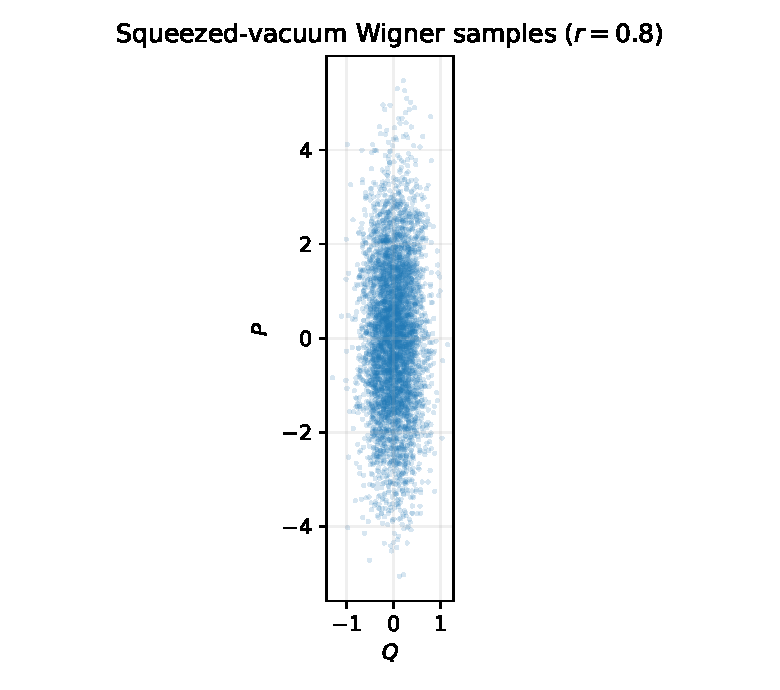
\includegraphics[width=0.72\textwidth]{figures/ch11/squeezed_wigner_sampling.pdf}
  \caption[压缩真空的 Wigner 抽样基准]{压缩参数 $r=0.8$ 时的单模压缩真空 Wigner 抽样。散点显示 $100000$ 个实际随机样本中的子集，椭圆给出解析高斯协方差；全样本协方差与反常矩的最大偏差分别为 $0.82$ 与 $0.84$ 个标准误以内。该图只验证单模高斯变换和抽样，不验证非高斯初态或后续相互作用动力学。}
  \label{fig:squeezed-sampling}
\end{figure}
图中的点是实际随机样本，不是示意性手绘；运行参数与数值误差保存在
\path{data/ch11/squeezed_sampling_metrics.json}。

\begin{chaptercheck}
把相互作用和传播时间都设为零，只运行初态生成器。若抽样的一、二阶矩不能在预期的 $N_s^{-1/2}$ 误差内复现输入协方差，就不应进入淬火模拟。初态偏差不会被更高阶积分器修复。
\end{chaptercheck}

\section*{本章小结}

相干态、热态和正高斯态可以直接由其实协方差精确抽样；Bogoliubov 初态还要求模式的辛归一化、零模处理与原子/准粒子基之间的一致转换。参数淬火会把普通协方差变成包含反常矩的压缩关联。固定粒子数和强非经典态则需要明确的近似或替代表示，不能靠轨迹重归一化假装精确。

\begin{exercises}
  \item 由式\eqref{eq:thermal-mode-sampling}计算 $Q,P$ 两个无量纲正交分量的方差。
  \item 证明式\eqref{eq:bogoliubov-map-constraints}保证变换后的 $c_\mu$ 仍满足玻色对易关系。
  \item 对单模压缩参数 $r$，取 $c=\cosh r\,b-\sinh r\,b^*$，求两个正交分量的方差与反常矩，并验证 $r>0$ 压缩 $Q$ 轴。
  \item 说明为什么逐轨迹归一化会在相干态中引入模式间关联。
  \item 为一个含 Goldstone 零模的 BdG 数值谱设计筛选、归一化和完备性检查。
\end{exercises}

\chapter{经典场传播与数值可信度}
\label{ch:propagation}

\begin{learningobjectives}
完成本章后，读者应能：
\begin{enumerate}
  \item 为 TWA 场方程选择与边界条件相符的传播算法；
  \item 推导 Fourier 分步法并说明其二阶精度与可逆性；
  \item 用守恒量、步长标度、反向传播和独立实现检验数值可信度；
  \item 组织可复现的随机轨迹并区分积分误差、截止误差和抽样误差。
\end{enumerate}
\end{learningobjectives}

\section{轨迹方程与量子近似是两层问题}

TWA 把量子演化近似成确定性经典场轨迹的系综。以第10章的一维格点方程为例，写成
\begin{equation}
  \ii\hbar\partial_t\psi
  =\left[T+V(x,t)+g(t)(|\psi|^2-\delta_{\mathcal C}(x,x))\right]\psi,
  \qquad
  T=-\frac{\hbar^2}{2m}\partial_x^2.
  \label{eq:propagation-field-equation}
\end{equation}
有限步长算法求解的是这条轨迹方程；丢弃高阶 Moyal 项则是把量子问题变成该方程的近似。前者收敛并不证明后者正确，但前者不收敛时，任何量子解释都失去基础。
投影经典场计算中的数值实践、截止依赖与热化风险可进一步参见
\cite{Blakie2008}。

以下讨论以闭合系统的确定性 TWA 为主。若主方程在 Wigner 表示中产生扩散，轨迹会变为随机微分方程，必须另行指定 It\^o 或 Stratonovich 解释；不能把本章的常微分方程积分器直接套用。

下文为简化排版记
$\delta_{\mathcal C}(x)\equiv\delta_{\mathcal C}(x,x)$。只有在等距、完整的
Fourier--DVR 网格上它才是常数 $1/\Delta x$；陷阱本征态截断、非均匀网格
或其他投影基一般给出随位置变化的对角投影核。代码若把它硬编码成一个
标量，就等于额外假设了均匀模式密度。

\section{Strang 分裂 Fourier 法}

周期边界下，把右端拆成动能 $T$ 与局域项
\begin{equation}
  U[\psi;t]=V(x,t)+g(t)(|\psi|^2-\delta_{\mathcal C}(x)).
\end{equation}
对时间无关参数，一个步长 $\Delta t$ 的 Strang 分裂为
\begin{equation}
  \psi(t+\Delta t)
  \approx
  \ee^{-\ii T\Delta t/(2\hbar)}
  \ee^{-\ii U\Delta t/\hbar}
  \ee^{-\ii T\Delta t/(2\hbar)}\psi(t).
  \label{eq:strang-splitting}
\end{equation}
动能指数在 Fourier 空间对角：
\begin{equation}
  \tilde\psi_k\longleftarrow
  \exp\!\left[-\ii\frac{\hbar k^2}{2m}\frac{\Delta t}{2}\right]
  \tilde\psi_k.
  \label{eq:kinetic-half-step}
\end{equation}
局域子步中 $|\psi(x)|^2$ 不变，因此可以精确写成相位乘法
\begin{equation}
  \psi(x)\longleftarrow
  \exp\!\left[-\frac{\ii\Delta t}{\hbar}
  \left(V(x)+g(|\psi(x)|^2-\delta_{\mathcal C}(x))\right)\right]\psi(x).
  \label{eq:local-nonlinear-step}
\end{equation}

若 $V$ 或 $g$ 随时间变化，应在子步中使用中点值 $t+\Delta t/2$，以保持整体二阶精度。式\eqref{eq:strang-splitting}的局域截断误差是 $\order(\Delta t^3)$，固定总时长的全局误差是 $\order(\Delta t^2)$；时间分裂谱方法在 Gross--Pitaevskii 方程中的系统分析和网格选择可参见\cite{Bao2003}。对时间无关、无滤波的实现，三个子步都是幺正的，因而离散范数在浮点误差内守恒；将 $\Delta t$ 换成 $-\Delta t$ 并逆序执行还能恢复初态。

\begin{warningbox}
范数守恒是必要测试，却不是精度证明。分步法的每个子步都可以严格守范数，即使步长大到相位和能量已经完全错误。必须再做步长标度和能量检查。
\end{warningbox}

\section{其他积分器何时更合适}

\subsection{有限差分与 Runge--Kutta}

复杂边界、非局域耦合或无法对角化的单粒子哈密顿量可先离散成
$\dot{\bm y}=\bm f(t,\bm y)$，再用 Runge--Kutta 法。显式 RK4 易实现，但对高波数动能是刚性的：稳定步长常随 $\Delta x^2$ 缩小。自适应高阶法可以控制局域误差，却通常不严格保持 Hamilton 结构和守恒量。

\subsection{隐式与结构保持方法}

Crank--Nicolson 对线性 Schr\"odinger 方程范数稳定；非线性问题需迭代求解。辛积分器或离散梯度方法更适合极长时间守恒研究，但每步成本可能更高。选择算法应由 Hamilton 结构、边界条件和目标时间尺度决定，而不是只比较单步速度。

\subsection{耦合分量}

双分量场的动能常仍可在 Fourier 空间传播，局域子步则包含一个 $2\times2$ 自旋哈密顿量。若 Rabi 耦合与非线性密度项不对易，可以在局域子步中对矩阵指数做解析或数值计算，或继续采用对称分裂。第14章将给出具体模型。

\section{投影、混叠与边界}

实空间乘积 $|\psi|^2\psi$ 会产生输入最高波数三倍的 Fourier 分量。有限网格无法表示这些分量，它们会以混叠形式折回低波数。处理方式包括：
\begin{enumerate}
  \item 把伪谱格点方程本身视为所定义的有限维模型，并通过加密网格检查；
  \item 对乘积使用零填充和去混叠规则；
  \item 每次计算非线性后显式施加 $\mathcal P_{\mathcal C}$。
\end{enumerate}
显式滤波若不是方程的一部分，会损失范数和能量；必须把它当作模型操作记录，而不是隐藏在“数值稳定化”中。

周期 Fourier 法还会让离开右边界的波包从左边界返回。研究膨胀或散射时，应增大计算域、在目标时间前停止，或加入经过反射测试的吸收层。吸收势使系统非 Hermitian，粒子数下降是建模结果而非积分误差。

\section{守恒量与可逆性测试}

对时间无关的闭合单分量模型，至少监测
\begin{align}
  \mathcal N_{\mathrm{sym}}&=\int\dd x\,|\psi|^2,\\
  N_W&=(\hat N)_W=\mathcal N_{\mathrm{sym}}-\frac M2,\\
  E_W&=\int\dd x\left[
  \frac{\hbar^2}{2m}|\partial_x\psi|^2+V|\psi|^2
  +\frac{g}{2}\left(|\psi|^4-2\delta_{\mathcal C}(x)|\psi|^2\right)
  \right],
  \label{eq:propagation-weyl-energy}
\end{align}
其中省略了不影响动力学的常数。$\mathcal N_{\mathrm{sym}}$ 是单条 Wigner
轨迹的原始对称范数；$N_W$ 才是扣除每模半量子后的粒子数 Weyl 符号，且
$\qavg{\hat N}=\ensavg{N_W}$。两者漂移相同，但输出时不能混用名称。

建议记录最大相对漂移而不只记录末时误差：
\begin{equation}
  \epsilon_Q=\max_{0\le t\le t_f}
  \frac{|Q(t)-Q(0)|}{\max(|Q(0)|,Q_{\rm scale})}.
  \label{eq:conservation-error}
\end{equation}
$Q_{\rm scale}$ 防止近零守恒量令相对误差失真。再做反向传播：从 $t_f$ 用 $-\Delta t$ 返回，测量
\begin{equation}
  \epsilon_{\rm rev}=
  \frac{\|\psi_{\rm back}-\psi_0\|_2}{\|\psi_0\|_2}.
  \label{eq:reversibility-error}
\end{equation}
该测试对 FFT 归一化、子步顺序和隐式滤波尤其敏感，但仍不能替代与精细步长解的比较。

\section{步长与空间收敛}

对二阶算法，分别用 $\Delta t,\Delta t/2,\Delta t/4$ 得到同一时刻的场。若进入渐近区，误差比应接近
\begin{equation}
  \frac{\|\psi_{\Delta t}-\psi_{\Delta t/2}\|}
       {\|\psi_{\Delta t/2}-\psi_{\Delta t/4}\|}
  \simeq 2^2=4.
  \label{eq:second-order-ratio}
\end{equation}
非线性相位可能让整体相位误差主导，因此还应对密度、关联函数等目标观测量重复这一检查。

空间收敛必须固定清楚比较对象。加密格点会改变 TWA 模式数和初始半量子总量；若目的是测试离散算符，可先关闭随机噪声并传播同一光滑场。若目的是测试完整 TWA 预测，则应按各自截止重新抽样，并比较物理估计器的系综统计量。两种实验回答不同问题。

\section{轨迹系综与随机数管理}

轨迹天然可并行，但可复现并不等于所有进程使用同一个种子。重复种子会制造完全相同的轨迹并虚增名义样本数。可靠方案是从一个主种子派生互不重叠的子流，例如用计数型生成器或 \texttt{SeedSequence.spawn}。每条轨迹的标识、子流编号、参数哈希和代码版本都应写入元数据。

在比较两个参数或两种算法时，使用共同随机数可以显著降低“差值”的方差：两次计算采用同一组初态样本，但各自独立传播。这样得到的两个均值是相关的，误差条必须基于逐轨迹差值计算，不能套用独立样本公式。

自适应积分会让不同轨迹具有不同内部时间点。观测量应在统一输出网格上由积分器插值，避免把相邻但不相同的时间混入一个系综平均。

\section{实际分步传播基准}

配套程序用一条带固定随机种子的格点 Wigner 场验证 Strang 分裂。它同时测量范数漂移、Weyl 能量漂移、正反传播误差和四档步长的二阶收敛，结果见\cref{fig:split-step-benchmark}。
\begin{figure}[htbp]
  \centering
  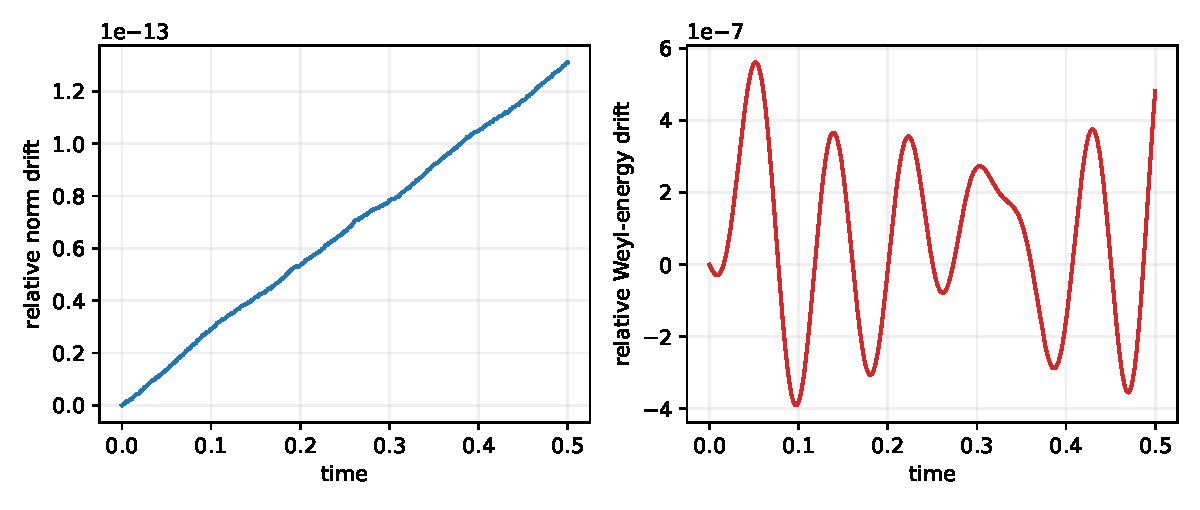
\includegraphics[width=0.78\textwidth]{figures/ch12/split_step_conservation.pdf}
  \caption[Strang 分裂传播的收敛与守恒基准]{周期区间 $L=20$ 上 $M=64$ 点单轨迹 Strang 分裂基准。步长 $\Delta t=0.004,0.002,0.001,0.0005$ 给出观测收敛阶 $2.001$；在记录步长 $\Delta t=0.001$ 下，范数漂移为 $1.31\times10^{-13}$、离散 Weyl 能量相对漂移为 $5.61\times10^{-7}$，正反传播误差为 $2.29\times10^{-13}$。该图验证离散积分器及其实现，不验证 TWA 的物理截断误差。}
  \label{fig:split-step-benchmark}
\end{figure}
这张图来自实际 FFT 传播；参数和误差保存在
\path{data/ch12/split_step_metrics.json}。该程序验证的是数值积分器，不是 TWA 对某个实验体系的物理准确性。

\begin{chaptercheck}
对每次生产运行保存四类互不替代的证据：时间步长表、空间/截止表、守恒与可逆性曲线、轨迹数与置信区间表。若只保存一条“结果曲线”和最终参数，事后无法判断偏差来自量子截断、数值积分还是 Monte Carlo 抽样。
\end{chaptercheck}

\section*{本章小结}

分步 Fourier 法利用动能和局域非线性的结构构造二阶、范数保持且可逆的传播，但仍需能量、步长标度和反向传播验证。投影、混叠、边界和随机数子流都是方程定义与可复现性的一部分。轨迹方程的数值收敛与 TWA 的量子有效性必须分别建立证据。

\begin{exercises}
  \item 用 Baker--Campbell--Hausdorff 公式说明对称分裂为何没有 $\order(\Delta t^2)$ 的单步误差项。
  \item 推导中心差分动能下显式 RK4 的稳定步长为何随 $\Delta x^2$ 缩小。
  \item 给式\eqref{eq:propagation-field-equation}加入时间依赖 $g(t)$，设计保持二阶精度的中点算法。
  \item 构造一个范数守恒但相位明显错误的大步长例子。
  \item 为双分量 Rabi 耦合的局域子步写出 $2\times2$ 矩阵指数。
\end{exercises}

\chapter{观测量、关联函数与误差条}
\label{ch:observables}

\begin{learningobjectives}
完成本章后，读者应能：
\begin{enumerate}
  \item 把 Wigner 轨迹上的对称排序量转换为正规排序观测量；
  \item 构造密度、一体相干、二阶关联、动量分布和结构因子；
  \item 为非线性与比值估计器计算不过度乐观的统计不确定度；
  \item 区分 Monte Carlo 误差、数值系统误差与方法误差。
\end{enumerate}
\end{learningobjectives}

\section{轨迹变量不是观测量本身}

Wigner 平均天然对应对称排序。实验和多体理论中常见的密度、粒子数和光子计数则是正规排序。第4章已经给出单模例子；对有限模式场，所有修正都由投影核 $\delta_{\mathcal C}(x,x')$ 决定。
相空间排序对应的系统综述见\cite{Hillery1984}；多分量投影场中的 functional
Wigner 估计器可与\cite{Opanchuk2013}核对。

一个稳健的分析流程应把三层对象分开：
\begin{enumerate}
  \item \textbf{原始轨迹量}，例如 $|\psi^{(s)}(x,t)|^2$；
  \item \textbf{逐轨迹或系综估计器}，包含排序修正；
  \item \textbf{最终统计量}，包含归一化、比值、拟合和置信区间。
\end{enumerate}
若把修正散落在绘图脚本中，同一数据很容易被两次扣除半量子或完全不扣除。

\section{密度与一体相干}

正规排序一体密度矩阵为
\begin{equation}
  G^{(1)}(x,x';t)
  =\qavg{\hpsid(x,t)\hpsi(x',t)}.
\end{equation}
其 Wigner 估计器是
\begin{equation}
  G^{(1)}(x,x';t)
  \approx
  \ensavg{\psi^*(x,t)\psi(x',t)}
  -\frac12\delta_{\mathcal C}(x,x').
  \label{eq:g1-wigner-estimator}
\end{equation}
令 $x'=x$ 得密度
\begin{equation}
  n(x,t)=\ensavg{|\psi(x,t)|^2}
  -\frac12\delta_{\mathcal C}(x,x).
  \label{eq:density-wigner-estimator}
\end{equation}
对正交格点，$\delta_{\mathcal C}(x_j,x_k)=\delta_{jk}/\Delta x$。不同格点的一体相干没有局域半量子扣除；同一点则必须扣除。

归一化一阶相干度通常定义为
\begin{equation}
  g^{(1)}(x,x')=
  \frac{G^{(1)}(x,x')}{\sqrt{n(x)n(x')}}.
  \label{eq:normalized-g1}
\end{equation}
应先分别估计分子和密度，再取比值；逐轨迹计算
$\psi^*(x)\psi(x')/[|\psi(x)||\psi(x')|]$ 回答的是相位因子问题，并不等于式\eqref{eq:normalized-g1}。

\section{二阶正规排序关联}

局域二阶关联的未归一化分子为
\begin{equation}
  G^{(2)}(x,x)
  =\qavg{\hpsid(x)^2\hpsi(x)^2}.
\end{equation}
对应的有限模式 Wigner 估计器是
\begin{equation}
  G^{(2)}(x,x)
  \approx\ensavg{
  |\psi|^4-2\delta_{\mathcal C}|\psi|^2
  +\frac12\delta_{\mathcal C}^2},
  \label{eq:local-g2-wigner-estimator}
\end{equation}
其中投影核均取 $(x,x)$。归一化二阶相干度为
\begin{equation}
  g^{(2)}(x,x)=\frac{G^{(2)}(x,x)}{n(x)^2}.
  \label{eq:normalized-g2}
\end{equation}
式\eqref{eq:local-g2-wigner-estimator}不是
$(|\psi|^2-\delta_{\mathcal C}/2)^2$；后者常数项为
$\delta_{\mathcal C}^2/4$，少了四次算符 Weyl 符号要求的另一项。

一般两点的正规排序分子
$G^{(2)}(x,x')=\qavg{\hpsid(x)\hpsid(x')\hpsi(x')\hpsi(x)}$
还包含非局域投影核。把所有场与投影核取在同一时刻，其 Wigner 估计器为
\begin{equation}
  G^{(2)}(x,x')\approx\ensavg{\begin{aligned}
  &|\psi(x)|^2|\psi(x')|^2
  -\frac12\delta_{\mathcal C}(x,x)|\psi(x')|^2
  -\frac12\delta_{\mathcal C}(x',x')|\psi(x)|^2 \\
  &-\frac12\delta_{\mathcal C}(x,x')\psi^*(x')\psi(x)
  -\frac12\delta_{\mathcal C}(x',x)\psi^*(x)\psi(x') \\
  &+\frac14\delta_{\mathcal C}(x,x)\delta_{\mathcal C}(x',x')
  +\frac14|\delta_{\mathcal C}(x,x')|^2
  \end{aligned}}.
  \label{eq:nonlocal-g2-general}
\end{equation}
令 $x'=x$ 即恢复式\eqref{eq:local-g2-wigner-estimator}。这一完整形式在
非正交投影基中尤其重要：即便两个坐标点不同，投影核也未必为零。

对两个不同的正交格点 $j\neq k$，正规排序关联可写成
\begin{equation}
  G^{(2)}_{jk}
  =\frac{1}{\Delta x^2}
  \ensavg{
  \left(|\alpha_j|^2-\frac12\right)
  \left(|\alpha_k|^2-\frac12\right)}.
  \label{eq:nonlocal-g2-grid}
\end{equation}
当 $j=k$ 时必须改用式\eqref{eq:local-g2-wigner-estimator}，因为同一模式的算符收缩多出接触项。

\section{动量分布与 Fourier 约定}

在 $M$ 点周期格点上定义归一化离散变换
\begin{equation}
  \alpha_\ell^{(k)}=\frac{1}{\sqrt M}
  \sum_{j=0}^{M-1}\ee^{-2\pi\ii j\ell/M}\alpha_j,
  \qquad
  \alpha_j=\sqrt{\Delta x}\,\psi_j.
  \label{eq:unitary-discrete-fourier}
\end{equation}
该变换保持 $\sum_j|\alpha_j|^2=\sum_\ell|\alpha_\ell^{(k)}|^2$。每个保留动量模式的占据为
\begin{equation}
  n_\ell^{(k)}=\ensavg{|\alpha_\ell^{(k)}|^2}-\frac12.
  \label{eq:momentum-occupation-estimator}
\end{equation}
许多数值 FFT 默认没有式\eqref{eq:unitary-discrete-fourier}的 $1/\sqrt M$ 对称归一化。代码必须在单模平面波上验证：实空间总粒子数、动量空间占据之和和 Parseval 恒等式三者一致。

连续动量密度 $n(k)$ 还涉及 Fourier 变换中的 $2\pi$ 约定及 $k$ 格距，不能仅把数组 $|\mathrm{FFT}(\psi)|^2$ 标成“占据”。正文、代码和图轴应明确画的是每个离散模式的粒子数还是单位波数的粒子密度。

\section{密度涨落与结构因子}

定义 $\delta\hat n(x)=\hat n(x)-n(x)$。静态结构因子可写成
\begin{equation}
  S(k)=\frac{1}{N}\int\dd x\dd x'\,
  \ee^{-\ii k(x-x')}
  \qavg{\delta\hat n(x)\delta\hat n(x')}.
  \label{eq:static-structure-factor}
\end{equation}
对第10章的投影场，密度算符乘积满足
\begin{equation}
  \qavg{\hat n_{\mathcal C}(x)\hat n_{\mathcal C}(x')}
  =G^{(2)}_{\mathcal C}(x,x')
  +\delta_{\mathcal C}(x,x')G^{(1)}_{\mathcal C}(x,x').
  \label{eq:density-shot-noise}
\end{equation}
右端第二项是粒子散粒噪声。在完整连续基极限，它退化为
$\delta(x-x')n(x)$。对均匀连续体系的非零波数，常用形式为
\begin{equation}
  S(k)=1+\frac{1}{N}\int\dd x\dd x'\,
  \ee^{-\ii k(x-x')}
  \left[G^{(2)}(x,x')-n(x)n(x')\right].
  \label{eq:structure-factor-normal-ordered}
\end{equation}
若用正规排序 $G^{(2)}$ 构造式\eqref{eq:structure-factor-normal-ordered}，就必须保留前面的 $1$；若直接从完整密度--密度关联出发，则不能再额外添加它。对有限投影基，应按式\eqref{eq:density-shot-noise}显式计算投影后的散粒噪声项，不能不加检查地把它替换成 $1$。

有限且不均匀体系的 $k=0$ 分量还包含总数涨落和非零平均密度 Fourier 分量，应使用式\eqref{eq:static-structure-factor}逐项计算，不宜套用均匀简式。

\section{序参量、条纹和有限尺寸}

密度波的复振幅可以定义为
\begin{equation}
  \rho_Q=\frac{1}{N}\int\dd x\,
  \ee^{-\ii Qx}n(x).
  \label{eq:density-wave-amplitude}
\end{equation}
若哈密顿量保持平移对称，而有限轨迹在随机位置形成条纹，系综平均 $\ensavg{\rho_Q}$ 可以因随机相位为零。此时
$\ensavg{|\rho_Q|^2}$ 或 $S(Q)$ 能检测有限尺寸密度关联，但其非零本身不证明热力学极限自发对称破缺。还需要随系统尺寸、粒子数、显式钉扎场和观测时间做标度。第17章将把这一点与超流响应结合。

相似地，先对每条轨迹寻找最大峰再平均会产生选择偏差，即使纯噪声也给出正“条纹对比度”。若峰位不是理论预先给定，应在独立数据上选窗，或把寻峰步骤完整纳入空模型与 bootstrap。

\section{统计误差条}

对 $N_s$ 条独立轨迹的标量估计器 $X_s$，样本均值和标准误为
\begin{equation}
  \bar X=\frac{1}{N_s}\sum_sX_s,
  \qquad
  {\rm SE}(\bar X)=
  \sqrt{\frac{1}{N_s(N_s-1)}\sum_s(X_s-\bar X)^2}.
  \label{eq:monte-carlo-standard-error}
\end{equation}
误差条反映有限轨迹，不包括时间步长、截止或 TWA 截断误差。

对 $R=A/B$、$g^{(2)}=G^{(2)}/n^2$ 等非线性统计量，不应先算每条轨迹的比值再平均。应从全体样本估计 $A,B$ 后取比值，并用按轨迹重抽样的 bootstrap 或 jackknife 传播其相关性。若 $B$ 接近零，比值分布可能强烈偏斜，此时对称的“均值正负一个标准差”会误导，应报告分位数区间或停止解释该区域。

空间格点和同一轨迹的多个时刻不是独立 Monte Carlo 样本。bootstrap 的基本重抽样单元应是完整轨迹；若初态来自 Markov 链，还须按自相关时间分块。

\section{多时关联的额外困难}

等时对称排序量可以直接由同一时刻轨迹计算。不同时间的普通量子乘积如
$\qavg{\hpsid(t)\hpsi(t')}$ 涉及算符顺序与响应，通常不等于简单的
$\ensavg{\psi^*(t)\psi(t')} $。受控计算可能需要 Bopp 算符、对初始条件的切线响应，或 Schwinger--Keldysh 路径上的插入。若只采用经典轨迹乘积，应明确它近似的是哪种半经典相关函数，不应默认为任意量子时间排序。

最简单的谐振子已经能看出差别。若
$\hat a(t)=\ee^{-\ii\omega t}\hat a(0)$，初态平均占据为 $\bar n$，则
\begin{align}
  \ensavg{\alpha^*(t)\alpha(t')}
  &=\left(\bar n+\frac12\right)\ee^{-\ii\omega(t'-t)},\\
  \qavg{\had(t)\ha(t')}
  &=\ensavg{\alpha^*(t)\alpha(t')}
  -\frac12\ee^{-\ii\omega(t'-t)}.
  \label{eq:two-time-harmonic-ordering}
\end{align}
这里的第二项是传播后的对易子，而不是只在 $t=t'$ 才出现的常数。对
非线性轨迹，该修正一般依赖切线响应
$\partial\alpha(t')/\partial\alpha(t)$，不能由一个通用的“减半量子”
规则替代。因此本书配套观测量程序只验证等时单模估计器；它没有验证
空间关联或任意多时量子关联。

\section{实际排序估计器基准}

配套程序分别抽样平均占据为 $4$ 的相干态和平均占据为 $2$ 的热态，用同一批轨迹计算密度、四阶正规排序矩与 $g^{(2)}$，结果见\cref{fig:ordering-estimator-benchmark}。
\begin{figure}[htbp]
  \centering
  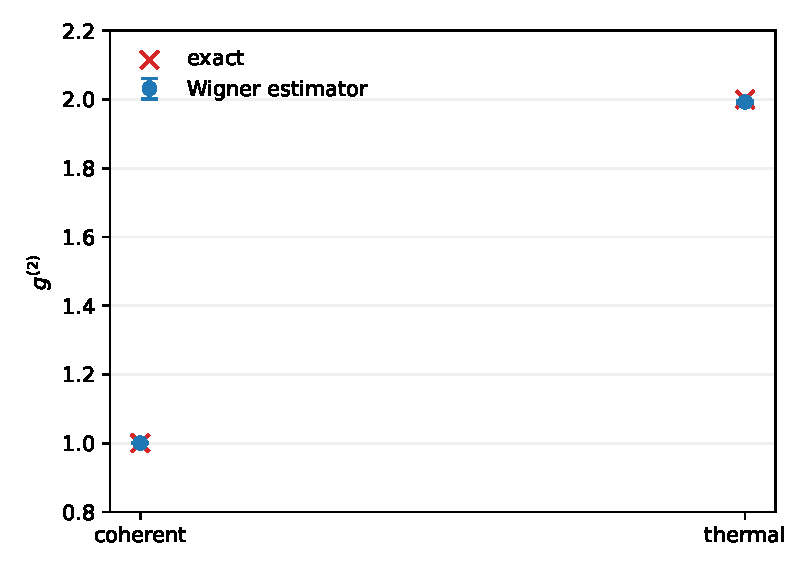
\includegraphics[width=0.72\textwidth]{figures/ch13/ordering_estimators.pdf}
  \caption[相干态与热态的正规排序估计器基准]{正规排序估计器的单模基准。相干态（$\bar n=4$）与热态（$\bar n=2$）各使用 $400000$ 个样本；$g^{(2)}$ 误差棒为 $200$ 组 jackknife 得到的 $\pm1$ 标准误。估计值分别为 $1.0002\pm0.0006$ 与 $1.9927\pm0.0049$，与解析值 $1$、$2$ 相容。该图不构成非局域关联、结构因子或多时响应实现的验证。}
  \label{fig:ordering-estimator-benchmark}
\end{figure}
相干态解析值为 $g^{(2)}=1$，热态为 $g^{(2)}=2$。程序使用分组 jackknife 给比值误差条，实际指标保存于
\path{data/ch13/ordering_estimator_metrics.json}。
这是排序公式的单模单元测试，不应被解释为式
\eqref{eq:nonlocal-g2-general}、结构因子或多时响应实现已经通过端到端验证。

\begin{chaptercheck}
为每张结果图附一张内部“误差预算表”：列出排序公式、轨迹数与统计误差、步长变化、截止变化、计算域变化和独立方法比较。最终正文可以压缩该表，但原始记录应保留，以免把很小的 Monte Carlo 误差条误当作总可信区间。
\end{chaptercheck}

\section*{本章小结}

Wigner 轨迹必须经过与算符排序相匹配的估计器才能变成物理观测量。密度扣除半个投影模式基线，局域四阶关联包含不同的二次与常数修正，结构因子还要正确处理散粒噪声。比值、寻峰和多时关联具有额外统计或算符顺序风险。轨迹误差条只度量 Monte Carlo 不确定度，不能覆盖数值、截止和方法误差。

\begin{exercises}
  \item 从单模四次算符的 Weyl 符号推导式\eqref{eq:local-g2-wigner-estimator}。
  \item 证明式\eqref{eq:unitary-discrete-fourier}保持原始对称范数
  $\mathcal N_{\mathrm{sym}}$，并说明固定模式数时为何也保持 $N_W$。
  \item 对相干态与热态分别计算 $g^{(2)}(0)$ 的解析值。
  \item 构造一个分母接近零的比值估计例子，比较 delta 方法与 bootstrap 区间。
  \item 说明为什么在每条噪声轨迹中搜索最大 Fourier 峰会产生正偏差，并设计一个空模型校准。
\end{exercises}


\part{双分量凝聚体的淬火动力学}
\chapter{双分量凝聚体的模型与对称性}
\label{ch:two-component-model}

\begin{learningobjectives}
完成本章后，读者应能：
\begin{enumerate}
  \item 区分均匀 Josephson/Rabi 耦合双组分模型与具有动量转移的 Raman 自旋轨道耦合模型；
  \item 由 Raman 单粒子哈密顿量求两条能带，并判断下带何时出现两个简并极小值；
  \item 从哈密顿量识别全局相位、相对相位、粒子数和平移对称性；
  \item 写出双分量接触相互作用的 TWA 场方程及正确 Weyl 修正；
  \item 判断参数淬火改变了哪些守恒量，以及哪些“条纹”结论不能由模型自动推出。
\end{enumerate}
\end{learningobjectives}

\section{最小双分量哈密顿量}

考虑准一维赝自旋分量 $L,R$，场算符满足
\begin{equation}
  \comm{\hat\Psi_\sigma(x)}{\hat\Psi_{\sigma'}^\dagger(x')}
  =\delta_{\sigma\sigma'}\delta(x-x').
\end{equation}
均匀线性耦合模型写成
\begin{align}
  \Hhat_0={}&\int\dd x\,
  \hat{\bm\Psi}^\dagger
  \left[h_0\identity_2+\frac{\delta}{2}\sigma_z-J\sigma_x\right]
  \hat{\bm\Psi},
  \qquad
  \hat{\bm\Psi}=\begin{pmatrix}\hat\Psi_L\\\hat\Psi_R\end{pmatrix},
  \label{eq:uniform-two-component-h0}\\
  \Hhat_{\rm int}={}&\int\dd x\left[
  \frac{g}{2}\left(
  \hat\Psi_L^{\dagger2}\hat\Psi_L^2+
  \hat\Psi_R^{\dagger2}\hat\Psi_R^2\right)
  +g_{12}\hat\Psi_L^\dagger\hat\Psi_R^\dagger
  \hat\Psi_R\hat\Psi_L\right],
  \label{eq:two-component-interaction}
\end{align}
其中 $h_0=-\hbar^2\partial_x^2/(2m)+V(x)$，$2J$ 是本书约定下单粒子对称与反对称态的能级劈裂，$\delta$ 是失谐。文献也常把 Rabi 频率记为 $\Omega=2J$；比较公式时必须先统一这一因子。

式\eqref{eq:uniform-two-component-h0}适用于内部态的零动量转移 Rabi 耦合，也适用于两条腿或两个局域模之间的 Josephson 耦合。它本身没有有限波矢，因而在均匀系统中不能单独选择一个非零条纹波数。

\section{Raman 耦合与自旋轨道项}

两束反向传播 Raman 光在实验室表象中产生带位置相位的耦合，例如
\begin{equation}
  -J\int\dd x\left(
  \ee^{2\ii k_Rx}\hat\Psi_L^\dagger\hat\Psi_R+{\rm h.c.}
  \right).
  \label{eq:raman-lab-coupling}
\end{equation}
通过自旋依赖规范变换去掉该相位后，单粒子哈密顿量可写成
\begin{equation}
  h_{\rm soc}=
  \frac{(p_x-\hbar k_R\sigma_z)^2}{2m}
  +\frac{\delta}{2}\sigma_z-J\sigma_x+V(x).
  \label{eq:raman-soc-hamiltonian}
\end{equation}
令 $E_R=\hbar^2k_R^2/(2m)$。在均匀空间中取 $p_x=\hbar k$，可把式\eqref{eq:raman-soc-hamiltonian}写成
\begin{equation}
  h_{\rm soc}(k)=\epsilon_0(k)\identity_2+d_z(k)\sigma_z-J\sigma_x,
  \quad
  \epsilon_0(k)=\frac{\hbar^2(k^2+k_R^2)}{2m},
  \quad
  d_z(k)=\frac{\delta}{2}-\frac{\hbar^2kk_R}{m}.
  \label{eq:soc-bloch-vector}
\end{equation}
因此两条单粒子能带为
\begin{equation}
  E_\pm(k)=\epsilon_0(k)\pm\sqrt{J^2+d_z(k)^2}.
  \label{eq:soc-single-particle-bands}
\end{equation}
这一步也固定了本书 $J$ 约定下的临界因子。零失谐时，$E_-(k)$ 在
\begin{equation}
  J<2E_R
  \label{eq:soc-double-minimum-condition}
\end{equation}
具有两个简并极小值
\begin{equation}
  k=\pm k_0,
  \qquad
  k_0=k_R\sqrt{1-\left(\frac{J}{2E_R}\right)^2};
  \label{eq:soc-minimum-wavevector}
\end{equation}
在 $J\geq2E_R$ 时两个极小值并合到 $k=0$。若采用实验文献常见的 $\Omega=2J$，同一条件写成 $\Omega<4E_R$。非零失谐一般使两个极小值不再简并，不能继续套用式\eqref{eq:soc-minimum-wavevector}。

设下带两个极小值的归一化自旋量为 $\chi_\pm$。相干叠加
\begin{equation}
  \bm\psi(x)=c_+\chi_+\ee^{\ii k_0x}
  +c_-\chi_-\ee^{-\ii k_0x}
  \label{eq:soc-two-minimum-superposition}
\end{equation}
在总密度中产生交叉项
\begin{equation}
  2\Re\!\left[c_+^*c_-\chi_+^\dagger\chi_-
  \ee^{-2\ii k_0x}\right].
  \label{eq:soc-stripe-overlap}
\end{equation}
故候选条纹波矢为 $Q=2k_0$，但振幅还取决于两个极小值是否同时宏观占据以及自旋量重叠 $\chi_+^\dagger\chi_-$。如果两自旋量正交，总密度交叉项消失，自旋密度仍可能调制。相互作用最终决定单极小值、双极小值相干叠加或其他相，而不是式\eqref{eq:soc-single-particle-bands}单独决定；这一模型结构和相图可参见实验与综述文献\cite{Lin2011,Li2012,Zhai2015}。

因此，后续章节将明确区分两条问题线：
\begin{enumerate}
  \item 式\eqref{eq:uniform-two-component-h0}的相对相位淬火、去相位与相分离动力学；
  \item 式\eqref{eq:raman-soc-hamiltonian}中由双极小值、相互作用和相干叠加共同形成的条纹候选态。
\end{enumerate}
均匀 $J$ 模型中的两分量相干性下降，不等同于 Raman 自旋轨道体系中条纹序的建立或消失。

\section{密度与自旋通道}

在平均场或正规排序层面定义
\begin{equation}
  n=n_L+n_R,
  \qquad
  s=n_L-n_R.
\end{equation}
对称耦合 $g_{LL}=g_{RR}=g$ 时，相互作用能密度可重写为
\begin{equation}
  \mathcal E_{\rm int}
  =\frac{g+g_{12}}{4}n^2
  +\frac{g-g_{12}}{4}s^2.
  \label{eq:density-spin-interaction}
\end{equation}
于是 $g+g_{12}$ 控制总密度通道的刚度，$g-g_{12}$ 控制自旋/相对密度通道。无 Rabi 耦合的均匀混合物在 $g_{12}>g$ 时对低波数自旋涨落不稳定，倾向于相分离；这并不自动意味着总密度形成周期条纹。Rabi 耦合、动能、有限尺寸与 SOC 带结构可以改变稳定边界，必须对具体模型求解。

写
\begin{equation}
  \psi_L=\sqrt{n_L}\ee^{\ii\theta_L},
  \qquad
  \psi_R=\sqrt{n_R}\ee^{\ii\theta_R},
  \qquad
  \phi=\theta_R-\theta_L,
\end{equation}
则均匀线性耦合能为
\begin{equation}
  \mathcal E_J=-2J\sqrt{n_Ln_R}\cos\phi.
  \label{eq:josephson-phase-energy}
\end{equation}
$J>0$ 把平衡相对相位钉扎在 $\phi=0$；相对密度 $s$ 是其共轭变量。大 $J$ 会增大相对相位涨落的恢复力，但“钉死”只是在低能近似中的说法，量子基态仍有有限宽度。

\section{对称性与守恒量账本}

\subsection{均匀线性耦合存在时}

全局变换 $\hat\Psi_{L,R}\to\ee^{\ii\chi}\hat\Psi_{L,R}$ 保持哈密顿量不变，总粒子数
$\hat N=\hat N_L+\hat N_R$ 守恒。若 $J\neq0$，独立的相对相位旋转不是对称性，$N_L-N_R$ 不守恒。均匀无陷阱时还具有连续平移对称和总动量守恒。

\subsection{淬火后关闭线性耦合}

若没有其他自旋翻转项，哈密顿量恢复
$U(1)_L\times U(1)_R$，$N_L$ 与 $N_R$ 分别守恒。相对相位不再被显式势能钉扎，但其空间梯度和相互作用仍产生动力学。一个瞬时淬火改变哈密顿量而不改变 $t=0$ 的量子态；对一般初始密度算符，新能量
\begin{equation}
  E_{\rm new}=\Tr(\rhohat_{\rm old}\Hhat_{\rm new})
  \label{eq:postquench-energy}
\end{equation}
随后守恒。纯态时才可把它写成相应的 bra--ket。它一般高于新哈密顿量基态能，差值是淬火注入能量，而不是与热浴交换的热量。

\subsection{Raman SOC 的对称性}

规范变换后的式\eqref{eq:raman-soc-hamiltonian}保持平移不变，但自旋与动量被锁定；实验室表象的普通平移要与 Raman 相位变换联合考虑。零失谐时还可能存在交换两个极小值的离散对称。条纹态涉及有限波矢密度相干，并可能破坏连续或由外场剩余的离散平移对称；具体对称群取决于 Raman 几何和边界。

\section{双分量 TWA 场方程}

在同一正交实空间格点上，双分量接触项的 Weyl 漂移并不完全相同。令
$\delta_{\mathcal C}=1/\Delta x$，则均匀耦合模型的闭合系统 TWA 为
\begin{align}
  \ii\hbar\partial_t\psi_L={}&\left[
  h_0+\frac{\delta}{2}
  +g(|\psi_L|^2-\delta_{\mathcal C})
  +g_{12}\left(|\psi_R|^2-\frac12\delta_{\mathcal C}\right)
  \right]\psi_L-J\psi_R,
  \label{eq:two-component-twa-l}\\
  \ii\hbar\partial_t\psi_R={}&\left[
  h_0-\frac{\delta}{2}
  +g(|\psi_R|^2-\delta_{\mathcal C})
  +g_{12}\left(|\psi_L|^2-\frac12\delta_{\mathcal C}\right)
  \right]\psi_R-J\psi_L.
  \label{eq:two-component-twa-r}
\end{align}
同分量四次项的漂移扣除一个投影基线；跨分量密度乘积的另一分量只扣除半个基线。这可由
\begin{equation}
  (\hat n_L\hat n_R)_W
  =\left(|\alpha_L|^2-\frac12\right)
   \left(|\alpha_R|^2-\frac12\right)
  \label{eq:cross-interaction-weyl}
\end{equation}
直接求导得到。双线性 $J$ 项是二次哈密顿量，不产生额外排序修正。

对 SOC 模型，记 $\bm\psi=(\psi_L,\psi_R)^T$，则两式可合写为
\begin{equation}
  \ii\hbar\partial_t\bm\psi
  =\left[h_{\rm soc}+\mathcal V_W(\bm\psi)\right]\bm\psi,
  \label{eq:soc-spinor-twa}
\end{equation}
其中 $\mathcal V_W$ 是由式\eqref{eq:two-component-twa-l}--\eqref{eq:two-component-twa-r}两个非线性对角元组成的矩阵。SOC 是二次单粒子项，不另产生 Weyl 修正；排序基线仍由实际保留的空间--自旋模式投影决定。

\subsection{可直接实现的 SOC 傅里叶传播器}

在均匀周期系统中，式\eqref{eq:soc-bloch-vector}给出每个 $k$ 上的精确单粒子步进
\begin{align}
  U_k(\Delta t)={}&\exp[-\ii\epsilon_0(k)\Delta t/\hbar]
  \left[
  \cos\!\left(\frac{\lambda_k\Delta t}{\hbar}\right)\identity_2
  -\ii\frac{\sin(\lambda_k\Delta t/\hbar)}{\lambda_k}
  \left(d_z(k)\sigma_z-J\sigma_x\right)
  \right],
  \label{eq:soc-fourier-propagator}\\
  \lambda_k={}&\sqrt{J^2+d_z(k)^2}.
\end{align}
$\lambda_k\to0$ 时应以解析极限或数值稳定的 $\operatorname{sinc}$ 实现第二项。一个 Strang 步可依次执行半个 $U_k$、完整的局域势与相互作用步、再半个 $U_k$。若局域步中还有不与密度矩阵对易的自旋翻转，需对相应 $2\times2$ 矩阵指数化，不能把两个分量各自乘相位。

规范变换也改变边界条件。实验室表象的场严格周期时，式\eqref{eq:raman-lab-coupling}在环上首先要求 $2k_RL\in2\pi\mathbb Z$；规范表象的两个自旋分量随后带相反的扭转因子 $\exp(\mp\ii k_RL)$。只有更强的条件 $k_RL\in2\pi\mathbb Z$ 成立时，两分量才同时适用普通周期 FFT；$k_RL$ 为奇数倍 $\pi$ 时则是反周期边界。一般情形应显式使用对应的扭曲动量网格，或直接在实验室表象传播式\eqref{eq:raman-lab-coupling}。初态噪声必须在同一个有限自旋--空间基中生成；若用 BdG 模抽样，正能模式、自旋量、粒子--空穴伙伴与传播器采用的规范和边界必须一致。

\section{无量纲控制参数}

均匀系统可用总密度 $n$ 和密度相互作用能
$E_n=n(g+g_{12})/2$ 建立尺度。常见无量纲量包括
\begin{equation}
  \gamma_s=\frac{g-g_{12}}{g+g_{12}},
  \qquad
  j=\frac{J}{E_n},
  \qquad
  \tilde\delta=\frac{\delta}{E_n},
  \qquad
  \kappa=\frac{\hbar^2k_R^2/(2m)}{E_n}.
\end{equation}
但真正的 TWA 风险还取决于每个截止模式的占据、系统长度、温度和淬火后演化时间。仅保持这些平均场比值相同，并不保证不同网格的量子涨落等价。

\section{模型建立检查表}

进入 BdG 或 TWA 前应逐项回答：
\begin{enumerate}
  \item $L,R$ 是内部态、空间双阱还是动量态？
  \item 线性耦合是否携带空间相位或动量转移？$J$ 与实验 Rabi 频率如何换算？
  \item $g,g_{12}$ 是哪一维度和哪种正规化约定下的参数？
  \item 淬火前后分别守恒哪些粒子数、动量和离散对称量？
  \item 条纹指总密度、自旋密度，还是释放后干涉图样？
  \item 候选有序相究竟破坏哪个 Hamilton 对称性？
\end{enumerate}

\begin{chaptercheck}
若只给出式\eqref{eq:uniform-two-component-h0}而没有 $k_R$、非局域相互作用、晶格或其他有限波矢机制，就不能把任何密度起伏自动解释成 Raman 条纹相。先从单粒子色散和线性稳定谱中证明存在目标波矢，再设计序参量。
\end{chaptercheck}

\section*{本章小结}

均匀 Josephson/Rabi 耦合与 Raman 自旋轨道耦合是不同模型：后者包含动量转移并可产生双极小值。$g_{12}>g$ 表示自旋通道趋向相分离，却不自动建立总密度条纹。淬火到 $J=0$ 恢复相对 $U(1)$ 对称并使两分量粒子数分别守恒。双分量 TWA 中，同分量和跨分量相互作用具有不同 Weyl 基线修正，必须在固定模式投影下实现。

\begin{exercises}
  \item 从 $n_L=(n+s)/2$、$n_R=(n-s)/2$ 推导式\eqref{eq:density-spin-interaction}。
  \item 对式\eqref{eq:uniform-two-component-h0}计算单粒子对称、反对称态能量并核对劈裂为 $2J$。
  \item 从式\eqref{eq:cross-interaction-weyl}推导式\eqref{eq:two-component-twa-l}中的跨分量修正。
  \item 列出 $J\neq0$ 与 $J=0$ 时所有连续对称性及对应守恒量。
  \item 说明实验室表象式\eqref{eq:raman-lab-coupling}怎样通过自旋依赖规范变换产生式\eqref{eq:raman-soc-hamiltonian}。
  \item 从式\eqref{eq:soc-single-particle-bands}求导，推导零失谐双极小值条件\eqref{eq:soc-double-minimum-condition}和位置\eqref{eq:soc-minimum-wavevector}。
  \item 证明式\eqref{eq:soc-fourier-propagator}是幺正矩阵，并实现 $\lambda_k\to0$ 时无除零误差的版本。
\end{exercises}

\chapter{Bogoliubov 模式与淬火协方差}
\label{ch:bogoliubov-quench}

\begin{learningobjectives}
完成本章后，读者应能：
\begin{enumerate}
  \item 把对称双分量凝聚体的线性涨落分解为密度与自旋通道；
  \item 由淬火前 Bogoliubov 真空构造淬火后的正常与反常协方差；
  \item 用旧基直接生成 Wigner 场样本，并检验新旧基之间的辛变换；
  \item 区分稳定准粒子压缩与动力学不稳定模的指数放大。
\end{enumerate}
\end{learningobjectives}

\section{均匀平衡背景}

本章采用标准弱涨落 Bogoliubov 线性化\cite{Dalfovo1999}。零模、有限体积
和数守恒问题需要更严格的投影处理\cite{Castin1998}；相干耦合双组分的物理
背景可参见\cite{Recati2022}。

先研究第14章均匀耦合模型，取失谐为零、无陷阱、总密度为 $n$，平均场背景为
\begin{equation}
  \psi_L^{(0)}=\psi_R^{(0)}=\sqrt{\frac n2}\,\ee^{-\ii\mu t/\hbar},
  \qquad
  \mu=\frac n2(g+g_{12})-J.
  \label{eq:balanced-two-component-background}
\end{equation}
定义对称与反对称涨落
\begin{equation}
  \delta\psi_d=\frac{\delta\psi_L+\delta\psi_R}{\sqrt2},
  \qquad
  \delta\psi_s=\frac{\delta\psi_L-\delta\psi_R}{\sqrt2}.
  \label{eq:density-spin-fluctuations}
\end{equation}
在 $g_{LL}=g_{RR}$、两分量平衡时，线性化哈密顿量在密度 $d$ 与自旋 $s$ 通道间分块对角。对自由色散
$\epsilon_k=\hbar^2k^2/(2m)$，下面把常被省略的中间步骤写出。先在旋转框架展开巨正则哈密顿量
$\hat K=\Hhat-\mu\hat N$，并令
\begin{equation}
  \delta\hat\Psi_c(x)=\frac1{\sqrt L}\sum_k\ha_{c,k}\ee^{\ii kx},
  \qquad c=d,s.
  \label{eq:density-spin-fourier-expansion}
\end{equation}
式\eqref{eq:balanced-two-component-background}使一阶项消失。把二阶项按无序波矢对 $\{k,-k\}$ 分组，可得
\begin{align}
  \hat K^{(2)}={}&\sum_{c=d,s}\sum_{k\in\mathcal K_+}
  A_{c,k}(\had_{c,k}\ha_{c,k}+\had_{c,-k}\ha_{c,-k})\notag\\
  &+\sum_{c=d,s}\sum_{k\in\mathcal K_+}
  B_{c,k}(\ha_{c,k}\ha_{c,-k}+\had_{c,k}\had_{c,-k})+\hat K_0,
  \label{eq:two-component-quadratic-pairs}\\
  A_{d,k}={}&\epsilon_k+\frac n2(g+g_{12}),
  &B_{d,k}={}&\frac n2(g+g_{12}),
  \label{eq:density-ab-coefficients}\\
  A_{s,k}={}&\epsilon_k+2J+\frac n2(g-g_{12}),
  &B_{s,k}={}&\frac n2(g-g_{12}).
  \label{eq:spin-ab-coefficients}
\end{align}
这里 $\mathcal K_+$ 从每一对非零波矢中只取一个代表；$\hat K_0$ 是必须单独处理的零模项。$2J$ 出现在自旋通道，是因为反对称单粒子态比凝聚的对称态高 $2J$；密度通道中的共同 $-J$ 已由化学势抵消。每个 $2\times2$ 动力学块满足
\begin{equation}
  \ii\hbar\partial_t
  \begin{pmatrix}\ha_{c,k}\\ \had_{c,-k}\end{pmatrix}
  =
  \begin{pmatrix}A_{c,k}&B_{c,k}\\-B_{c,k}&-A_{c,k}\end{pmatrix}
  \begin{pmatrix}\ha_{c,k}\\ \had_{c,-k}\end{pmatrix}.
  \label{eq:channel-bdg-dynamical-block}
\end{equation}
特征方程是 $E_{c,k}^2=A_{c,k}^2-B_{c,k}^2$，所以两支能谱为
\begin{align}
  E_d(k)^2&=\epsilon_k\left[\epsilon_k+n(g+g_{12})\right],
  \label{eq:density-bogoliubov-dispersion}\\
  E_s(k)^2&=(\epsilon_k+2J)
  \left[\epsilon_k+2J+n(g-g_{12})\right].
  \label{eq:spin-bogoliubov-dispersion}
\end{align}
密度支不依赖均匀 $J$，因为背景化学势与对称单粒子能量的 $J$ 位移抵消。自旋支在 $J>0$ 时有能隙；关闭 $J$ 后，若 $g_{12}<g$，它成为稳定的线性色散 Goldstone 模；若 $g_{12}>g$，一段低波数范围满足 $E_s^2<0$，背景发生动力学相分离不稳定。

\section{单个通道的 Bogoliubov 变换}

对每个通道与成对波矢 $\pm k$，二次哈密顿量可写成
\begin{equation}
  \Hhat_k^{(2)}=
  A_k(\had_k\ha_k+\had_{-k}\ha_{-k})
  +B_k(\ha_k\ha_{-k}+\had_k\had_{-k})+{\rm const.}
  \label{eq:paired-bogoliubov-hamiltonian}
\end{equation}
在 $A_k>|B_k|$ 时，$E_k=\sqrt{A_k^2-B_k^2}$ 为实数。取实系数约定
\begin{equation}
  \ha_k=u_k\hb_k-v_k\hbd_{-k},
  \qquad
  u_k^2-v_k^2=1,
  \label{eq:single-channel-bogoliubov-map}
\end{equation}
可选
\begin{equation}
  u_k=\sqrt{\frac12\left(\frac{A_k}{E_k}+1\right)},
  \qquad
  v_k={\rm sgn}(B_k)
  \sqrt{\frac12\left(\frac{A_k}{E_k}-1\right)}.
  \label{eq:bogoliubov-uv}
\end{equation}
若更换式\eqref{eq:single-channel-bogoliubov-map}中 $v$ 的符号约定，后续反常矩符号也会改变，但可观测协方差不变。代码中不应只保存 $E_k$；还要保存完整的模式相位与辛归一化约定。

式\eqref{eq:density-ab-coefficients}和\eqref{eq:spin-ab-coefficients}代入 $E_k^2=A_k^2-B_k^2$，分别复现式\eqref{eq:density-bogoliubov-dispersion}和\eqref{eq:spin-bogoliubov-dispersion}。这也说明两式不是独立记忆公式，而是同一个辛 $2\times2$ 块在两个通道中的结果。

\paragraph{$\pm k$ 的计数规则。}
式\eqref{eq:two-component-quadratic-pairs}若只对 $\mathcal K_+$ 求和，括号中必须同时保留 $k$ 与 $-k$；若改成对全部非零 $k$ 求和，整个成对哈密顿量要乘 $1/2$。抽样时 $b_k$ 与 $b_{-k}$ 是两个独立复高斯变量，不能因实值 Fourier 场的习惯而错误设置 $b_{-k}=b_k^*$：玻色场本身是复场。粒子--空穴伙伴只负责补全 Nambu 基，不再引入一套独立随机变量。$k=0$ 既等于自身的反向波矢，又可能是 Goldstone 模，必须从成对循环中剔除并按所选粒子数系综单独处理。

\section{突然淬火产生两模压缩}

设淬火前后参数分别记为 $i,f$。同一通道的两套系数是
$(u_{i,k},v_{i,k})$ 和 $(u_{f,k},v_{f,k})$。消去原子涨落算符后，新旧准粒子满足
\begin{equation}
  c_k=\mathcal A_k b_k+\mathcal B_k b_{-k}^\dagger,
  \label{eq:quench-mode-map}
\end{equation}
其中在上述实系数约定下
\begin{equation}
  \mathcal A_k=u_{f,k}u_{i,k}-v_{f,k}v_{i,k},
  \qquad
  \mathcal B_k=v_{f,k}u_{i,k}-u_{f,k}v_{i,k},
  \label{eq:quench-ab-coefficients}
\end{equation}
并满足 $\mathcal A_k^2-\mathcal B_k^2=1$。若初态是旧准粒子真空，则
\begin{equation}
  \qavg{\hat c_k^\dagger\hat c_k}=\mathcal B_k^2,
  \qquad
  \qavg{\hat c_k\hat c_{-k}}=\mathcal A_k\mathcal B_k,
  \label{eq:postquench-normal-anomalous}
\end{equation}
这里为简洁把新准粒子算符记作 $\hat c_k$。第一项是淬火产生的模式占据，第二项是相反动量之间的反常配对关联。对应量子态是相对于新真空的两模压缩高斯态。

有限温旧态的占据为 $\bar n_{i,k}$ 时，式\eqref{eq:postquench-normal-anomalous}推广为
\begin{align}
  \qavg{\hat c_k^\dagger\hat c_k}
  &=(\mathcal A_k^2+\mathcal B_k^2)\bar n_{i,k}+\mathcal B_k^2,\\
  \qavg{\hat c_k\hat c_{-k}}
  &=(2\bar n_{i,k}+1)\mathcal A_k\mathcal B_k.
  \label{eq:finite-temperature-quench-covariance}
\end{align}

\section{Wigner 协方差与直接抽样}

在 Wigner 表示中，旧准粒子样本为
\begin{equation}
  b_k=\sqrt{\frac{\bar n_{i,k}+1/2}{2}}
  (\xi_{1k}+\ii\xi_{2k}).
  \label{eq:old-mode-wigner-sample}
\end{equation}
把式\eqref{eq:quench-mode-map}中的算符替换为复数及其共轭，得到
\begin{equation}
  c_k=\mathcal A_k b_k+\mathcal B_k b_{-k}^*.
  \label{eq:new-mode-wigner-sample}
\end{equation}
其对称排序矩为
\begin{align}
  \ensavg{|c_k|^2}
  &=(\bar n_{i,k}+1/2)(\mathcal A_k^2+\mathcal B_k^2),\\
  \ensavg{c_kc_{-k}}
  &=(2\bar n_{i,k}+1)\mathcal A_k\mathcal B_k.
  \label{eq:new-mode-wigner-covariance}
\end{align}
第一式减去 $1/2$ 后正好得到式\eqref{eq:finite-temperature-quench-covariance}的正常占据。

实际 TWA 不必先生成新准粒子。更直接且较少出错的方法是用淬火前 BdG 模抽样，并立即重构原子场：
\begin{equation}
  \psi_\sigma(x,0)=\psi_\sigma^{(0)}(x)
  +\sum_{\nu\in\mathcal B_i}
  \left[u^{(i)}_{\sigma\nu}(x)b_\nu
  -v^{(i)*}_{\sigma\nu}(x)b_\nu^*\right].
  \label{eq:old-bdg-direct-field-sampling}
\end{equation}
随后直接用新哈密顿量的非线性场方程传播。新基协方差主要用于解析解释和抽样验收，而不是必需的中间数据格式。

\section{一般非均匀 BdG 问题}

在陷阱、SOC 或不对称耦合下，密度/自旋分块通常失效。设离散后有 $M$ 个空间--自旋单粒子模式。为与式\eqref{eq:old-bdg-direct-field-sampling}的负号约定一致，正能列及其粒子--空穴伙伴统一写成
\begin{equation}
  \bm w_\nu=\begin{pmatrix}\bm u_\nu\\-\bm v_\nu\end{pmatrix},
  \qquad
  \bar{\bm w}_\nu=\tau_x\bm w_\nu^*
  =\begin{pmatrix}-\bm v_\nu^*\\\bm u_\nu^*\end{pmatrix},
  \qquad
  \bm u_\nu=(u_{L\nu},u_{R\nu},\ldots)^T.
  \label{eq:general-bdg-mode-sign-convention}
\end{equation}
线性化方程具有广义辛本征结构
\begin{equation}
  \mathcal L\bm w_\nu=\epsilon_\nu\bm w_\nu,
  \qquad
  \bm w_\nu^\dagger\Sigma_z\bm w_\mu=\delta_{\nu\mu},
  \qquad
  \Sigma_z=\diag(\identity_M,-\identity_M).
  \label{eq:spinor-bdg-symplectic-norm}
\end{equation}
离散后要用与 TWA 相同的格点内积、规范和边界条件。普通 Euclidean 归一化 $\bm w^\dagger\bm w=1$ 不能保证准粒子对易关系。若 $\bm w_\nu$ 是能量 $+\epsilon_\nu$、辛范数 $+1$ 的模式，则式\eqref{eq:general-bdg-mode-sign-convention}中的 $\bar{\bm w}_\nu$ 具有能量 $-\epsilon_\nu$ 和辛范数 $-1$，其中 $\tau_x$ 交换 Nambu 的上下两块。

令 $U=(\bm u_1,\ldots,\bm u_M)$、$V=(\bm v_1,\ldots,\bm v_M)$。只有把 $M$ 个正范数模式及其 $M$ 个粒子--空穴伙伴同时放入，才得到可逆的完整伪幺正（paraunitary）矩阵
\begin{equation}
  \begin{aligned}
    \bm{\mathcal A}&=S\bm\beta,
    &\bm{\mathcal A}&=\begin{pmatrix}\bm a\\\bm a^\dagger\end{pmatrix},
    &\bm\beta&=\begin{pmatrix}\bm b\\\bm b^\dagger\end{pmatrix},\\
    S&=(\bm w_1,\ldots,\bm w_M,
    \bar{\bm w}_1,\ldots,\bar{\bm w}_M)
    =\begin{pmatrix}U&-V^*\\-V&U^*\end{pmatrix}.
  \end{aligned}
  \label{eq:complete-paraunitary-matrix}
\end{equation}
它必须满足
\begin{equation}
  S^\dagger\Sigma_zS=\Sigma_z,
  \qquad
  S^{-1}=\Sigma_zS^\dagger\Sigma_z,
  \qquad
  SS^{-1}=\identity_{2M}.
  \label{eq:paraunitary-identities}
\end{equation}
只把正能列排成一个 $2M\times M$ 矩阵时没有普通逆矩阵，不能直接写 $S^{-1}$。对淬火前后两个完整基，原子 Nambu 向量同时满足 $\bm{\mathcal A}=S_i\bm\beta_i=S_f\bm\beta_f$，所以
\begin{equation}
  \bm\beta_f=S_f^{-1}S_i\bm\beta_i.
  \label{eq:general-bdg-basis-map}
\end{equation}
用矩阵形式计算比逐个手写重叠公式更能容纳复模式、SOC 和简并子空间。简并正能子空间内还允许任意幺正旋转，因此跨参数匹配模式时应比较整个子空间投影，而不是依赖单列的相位或排序。严格零模、Jordan 块和复频不稳定模不能塞入上述普通 paraunitary 对角化；它们应先被投影出来，分别用数守恒集体坐标或线性辛时间传播处理。

\section{稳定压缩与不稳定放大}

“旧真空是新基中的压缩态”要求新二次哈密顿量存在实频率、正范数的稳定准粒子基。若式\eqref{eq:spin-bogoliubov-dispersion}给出 $E_s(k)^2<0$，相应模的频率为虚数，不存在以该不稳定背景为中心的正规新真空。此时仍可从旧态协方差出发，但应直接用线性辛传播
\begin{equation}
  V(t)=S_f(t)V(0)S_f(t)^T
  \label{eq:linear-covariance-propagation}
\end{equation}
或完整 TWA 演化。早期涨落指数增长是动力学不稳定，而不是平稳压缩准粒子振荡。非线性随后会饱和增长并耦合其他模式。

关闭 $J$ 还会使均匀自旋支的 $k=0$ 模成为零模。其 $u,v$ 在热力学参数化中可能发散，不能机械代入式\eqref{eq:bogoliubov-uv}。应改用相对相位--相对数的集体坐标，固定守恒粒子数扇区，或在有限体积数守恒 BdG 中单独处理。

\section{实际淬火协方差基准}

配套程序选取稳定参数 $g=1$、$g_{12}=0.6$，把均匀耦合从
$J_i=1$ 淬火到 $J_f=0.1$。程序直接抽样旧自旋准粒子真空，再变换到新基，比较正规占据和反常矩，结果见\cref{fig:bdg-quench-covariance}。
\begin{figure}[htbp]
  \centering
  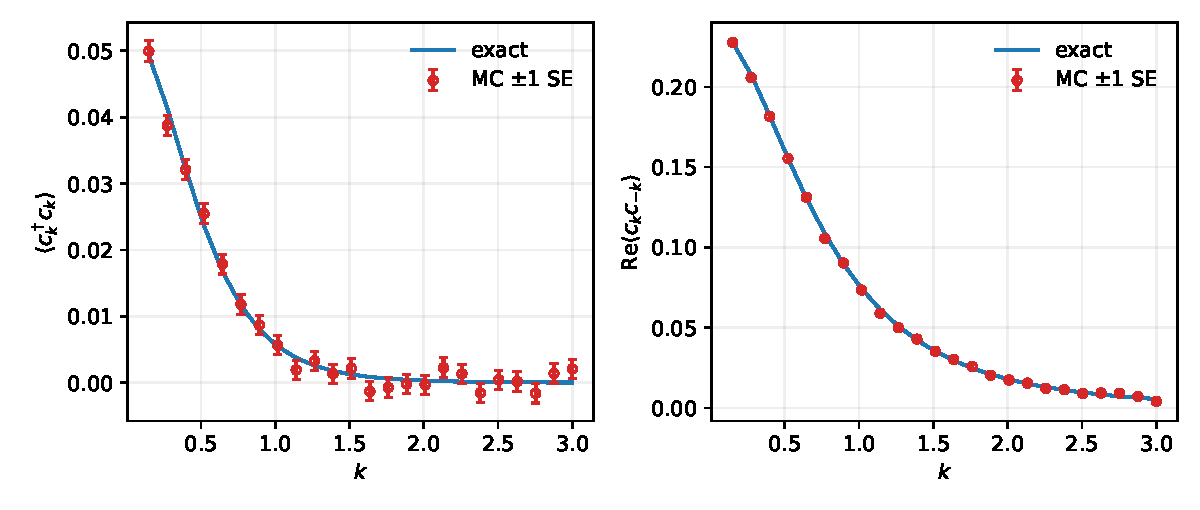
\includegraphics[width=0.78\textwidth]{figures/ch15/quench_covariance.pdf}
  \caption[BdG 淬火的正规与反常协方差基准]{在 $n=1$、$g=1$、$g_{12}=0.6$ 下，稳定自旋支从 $J_i=1$ 淬火到 $J_f=0.1$ 后的新基协方差。24个动量点各使用 $120000$ 对旧基真空样本，点的误差棒为 $\pm1$ 标准误，曲线为解析 Bogoliubov 变换；正规占据和反常矩的最大绝对误差分别为 $2.62\times10^{-3}$、$2.88\times10^{-3}$。同一运行还验收完整 paraunitary 矩阵、辛逆和原子场协方差；该图不覆盖零模或虚频不稳定区。}
  \label{fig:bdg-quench-covariance}
\end{figure}
图中点来自实际高斯 Monte Carlo；解析曲线由式\eqref{eq:quench-ab-coefficients}--\eqref{eq:new-mode-wigner-covariance}给出。全部参数与最大误差保存在
\path{data/ch15/quench_covariance_metrics.json}。同一程序还逐动量构造完整 $4\times4$
矩阵 $S_i,S_f$，验收 paraunitary 恒等式、辛逆矩阵、新旧基映射，以及由新旧基
重构原子 Nambu 协方差的一致性；因此图中的两条准粒子矩曲线不是唯一的通过条件。

\begin{chaptercheck}
完成 BdG 求解后先做四项机器测试：正负能成对、辛范数为正负一、不同正能模辛正交、由全部保留模重构投影单位算符。随后用至少一个稳定淬火比较“旧基直接抽样”和“新基协方差抽样”的原子场一、二阶矩。
\end{chaptercheck}

\section*{本章小结}

对称双分量凝聚体的线性涨落分成密度与自旋支，均匀耦合主要给自旋支开隙。稳定参数淬火把旧准粒子真空映射为新基中的两模压缩态，其正常与反常协方差由一个辛 Bogoliubov 变换确定。实际 TWA 可直接在旧基抽样并重构原子场。若新谱含虚频或零模，则应使用集体坐标或协方差传播，不能假定存在普通的新准粒子真空。

\begin{exercises}
  \item 从原始双分量哈密顿量逐项展开到式\eqref{eq:two-component-quadratic-pairs}，特别核对 $2J$、配对项以及只取 $\mathcal K_+$ 时的因子。
  \item 证明式\eqref{eq:quench-ab-coefficients}满足 $\mathcal A_k^2-\mathcal B_k^2=1$。
  \item 由式\eqref{eq:new-mode-wigner-sample}推导有限温协方差式\eqref{eq:new-mode-wigner-covariance}。
  \item 从式\eqref{eq:complete-paraunitary-matrix}证明式\eqref{eq:paraunitary-identities}，并说明为什么只保留正能列后不能求普通逆。
  \item 求 $J_f=0$、$g_{12}>g$ 时虚频波数区间。
  \item 设计一个数值测试，区分不稳定模的指数增长与稳定压缩模的周期振荡。
\end{exercises}

\chapter{相位扩散、模式耦合与预热化}
\label{ch:phase-dynamics}

\begin{learningobjectives}
完成本章后，读者应能：
\begin{enumerate}
  \item 区分全局相位扩散、有限波数去相位和非线性碰撞再分配；
  \item 由相对数涨落推导相干因子的高斯衰减；
  \item 用模式占据、反常关联和守恒量识别预热化时间窗；
  \item 说明为什么非线性 TWA 轨迹中的阻尼不能单独证明不可逆量子热化。
\end{enumerate}
\end{learningobjectives}

\section{三种容易混淆的“失相干”}

关闭线性耦合后，跨分量相干
\begin{equation}
  C_{LR}(t)=
  \frac{\int\dd x\,\qavg{\hat\Psi_L^\dagger(x,t)\hat\Psi_R(x,t)}}
  {\sqrt{\qavg{\hat N_L}\qavg{\hat N_R}}}
  \label{eq:intercomponent-coherence}
\end{equation}
通常下降，但至少有三种不同机制：
\begin{enumerate}
  \item \textbf{全局相位扩散}：不同相对粒子数分量具有不同化学势差；
  \item \textbf{线性模式去相位}：不同 $k$ 的稳定 Bogoliubov 模以不同频率旋转；
  \item \textbf{非线性模式耦合}：三波、四波过程改变模式占据并可能建立动理学松弛。
\end{enumerate}
它们可以在同一曲线上叠加，却对应不同可逆性、尺寸标度和理论近似。只拟合一个指数衰减常数不能识别机制。

跨分量算符 $\hat\Psi_L^\dagger\hat\Psi_R$ 已是两个不同正则模式的双线性乘积，其 Wigner 估计器直接是
$\ensavg{\psi_L^*\psi_R}$，没有同分量密度的半量子接触扣除。

\section{零模的相位扩散}

令相对数差为 $\delta N=(N_L-N_R)/2$，相对相位为
$\phi=\theta_R-\theta_L$。在小涨落集体坐标中，淬火前可写成
\begin{equation}
  H_{\rm rel}=\frac{E_C}{2}(\delta N)^2
  +\frac{E_J}{2}\phi^2,
  \label{eq:relative-collective-hamiltonian}
\end{equation}
其中 $E_J$ 来自式\eqref{eq:josephson-phase-energy}在极小值附近的展开。关闭 $J$ 后取 $E_J=0$，Hamilton 方程给出
\begin{equation}
  \delta N(t)=\delta N(0),
  \qquad
  \phi(t)=\phi(0)+\frac{E_Ct}{\hbar}\delta N(0).
  \label{eq:phase-diffusion-trajectory}
\end{equation}
若初态是高斯，便有
\begin{align}
  \Var[\phi(t)]={}&\Var[\phi(0)]
  +2\frac{E_Ct}{\hbar}\Cov[\phi(0),\delta N(0)]
  +\left(\frac{E_Ct}{\hbar}\right)^2\Var[\delta N(0)].
  \label{eq:phase-variance-growth}
\end{align}
当均值为零时，圆相干因子为
\begin{equation}
  \qavg{\ee^{\ii\phi(t)}}
  =\exp\!\left[-\frac12\Var[\phi(t)]\right].
  \label{eq:gaussian-phase-coherence}
\end{equation}
若初始交叉协方差可忽略，可定义尺度
\begin{equation}
  \tau_\phi=\frac{\hbar}{E_C\sqrt{\Var(\delta N)}}.
  \label{eq:phase-diffusion-time}
\end{equation}
它控制高斯包络，而不是普适的指数寿命。

相位扩散来自相对数的不确定度，但这里必须区分精确量子态与半经典相位包。精确的 $\delta N$ 本征态没有一个同时确定的共轭相对相位；其相位表象概率在圆上展开，不能把式\eqref{eq:phase-diffusion-trajectory}解释为“一个确定相位沿轨迹转动”。若初态是窄但非零宽度的数压缩半经典波包，且没有空间模式或其他噪声使化学势差变化，每个样本才近似作确定性转动，系综展宽由实际的 $\Var(\delta N)$ 决定。相干态抽样天然含相对数涨落；固定数差的精确态则需要周期相位表示或数守恒方法，普通 Cartesian 高斯近似只在远离圆周绕回且涨落近似连续的时间窗内适用。

有限量子转子的数谱离散，长时间可以出现回复。把 $\delta N$ 当连续变量的高斯 TWA 能准确描述早期展开，却通常丢失离散谱干涉造成的精确回复。这与第6章 Kerr 反例是同一种限制。

\section{空间相位场与线性去相位}

低能自旋通道可用相对相位 $\phi(x)$ 与相对密度 $s(x)$ 描述：
\begin{equation}
  H_s^{(2)}=\frac12\int\dd x\left[
  \chi_s^{-1}s(x)^2+\rho_s(\partial_x\phi)^2
  +M_J^2\phi(x)^2\right].
  \label{eq:spin-hydrodynamic-hamiltonian}
\end{equation}
$M_J$ 在耦合关闭后消失。每个稳定 Fourier 模都是独立谐振子；第15章的淬火协方差在这些模式中旋转。局域相干满足高斯恒等式
\begin{equation}
  \qavg{\ee^{\ii[\phi(x,t)-\phi(x',t)]}}
  =\exp\!\left[-\frac12
  \qavg{[\phi(x,t)-\phi(x',t)]^2}\right].
  \label{eq:gaussian-spatial-coherence}
\end{equation}
不同波数的非公度频率会使简单观测量趋于平滑平台，即使每个模式占据在严格二次理论中保持不变。这是相位混合或去相位，不是能量在模式间碰撞转移。

在近线性色散中，关联变化还会呈现有限传播速度形成的“光锥”结构。计算域必须大到使该前沿在分析窗口内不绕过周期边界。

\section{预热化平台}

若存在时间尺度分离
\begin{equation}
  \tau_{\rm dephase}\ll t\ll\tau_{\rm collision},
  \label{eq:prethermal-window}
\end{equation}
局域观测量可能已经近似平稳，而近似守恒的线性模式占据仍保留初态信息。这一中间状态称为预热化平台；孤立一维量子气体中已有相应实验观测\cite{Gring2012}。它常可由高斯协方差或广义统计系综描述，但“有效温度”可能依赖观测通道和波数范围。

识别预热化至少应同时展示：
\begin{enumerate}
  \item 一些实空间观测量已进入平台；
  \item 线性模式占据在该窗口内近似不变；
  \item 反常关联通过去相位下降或振荡平均；
  \item 更晚时非线性占据再分配尚未显著；
  \item 平台随系统尺寸和截止的变化受控。
\end{enumerate}

\section{非线性模式耦合}

把完整哈密顿量在凝聚背景附近展开，除了 $H^{(2)}$ 外还有
\begin{equation}
  H=H^{(0)}+H^{(2)}+H^{(3)}+H^{(4)}+\cdots.
\end{equation}
$H^{(3)}$ 允许满足能量--动量条件的一模衰变为两模及其逆过程，通常与 Beliaev 和 Landau 过程相关；$H^{(4)}$ 产生四波散射与频率重整化。是否存在共振取决于实际色散、维数、陷阱和 SOC，自旋“Cherenkov 发射”不是所有双分量模型的普适标签。

非线性 GPE/TWA 轨迹确实包含这些经典场模式耦合顶角，无需手工附加碰撞项。但由此观察到模式占据变化，只能说明所模拟的截断经典场发生了再分配。要把速率解释成量子 Beliaev--Landau 碰撞，还需在弱耦合重叠区与量子动理学或微扰计算比较，并检查每个参与模式的占据与截止依赖。

\section{“不可逆”需要操作定义}

闭合 TWA 轨迹的 Hamilton 流是微观可逆的。若保存终态并用负时间步长精确反演，理想数值程序应回到初态；系综平均阻尼来自相空间剪切、混合和信息粗粒化。真正的实验不可逆性可以由不可控自由度、开放系统或热力学极限中的极长回归时间产生，但不能由一条平滑衰减曲线单独证明。

可以设计三类区分实验：
\begin{enumerate}
  \item \textbf{回波}：在 $t_e$ 反转可控 Hamilton 参数，检查相干是否恢复；
  \item \textbf{占据账本}：区分固定占据的去相位与随时间改变的碰撞再分配；
  \item \textbf{分布检验}：比较晚时模式分布与 Bose--Einstein、Rayleigh--Jeans 及广义系综，并做截止稳定性。
\end{enumerate}
TWA 的晚时经典场常趋向截止相关的 Rayleigh--Jeans 型分布，因此仅凭“拟合出温度”不能声称量子热化。

\section{实际相位扩散基准}

配套程序对式\eqref{eq:phase-diffusion-trajectory}抽样 $2\times10^5$ 条高斯轨迹，并与式\eqref{eq:phase-variance-growth}和\eqref{eq:gaussian-phase-coherence}比较，结果见\cref{fig:phase-diffusion-benchmark}。
\begin{figure}[htbp]
  \centering
  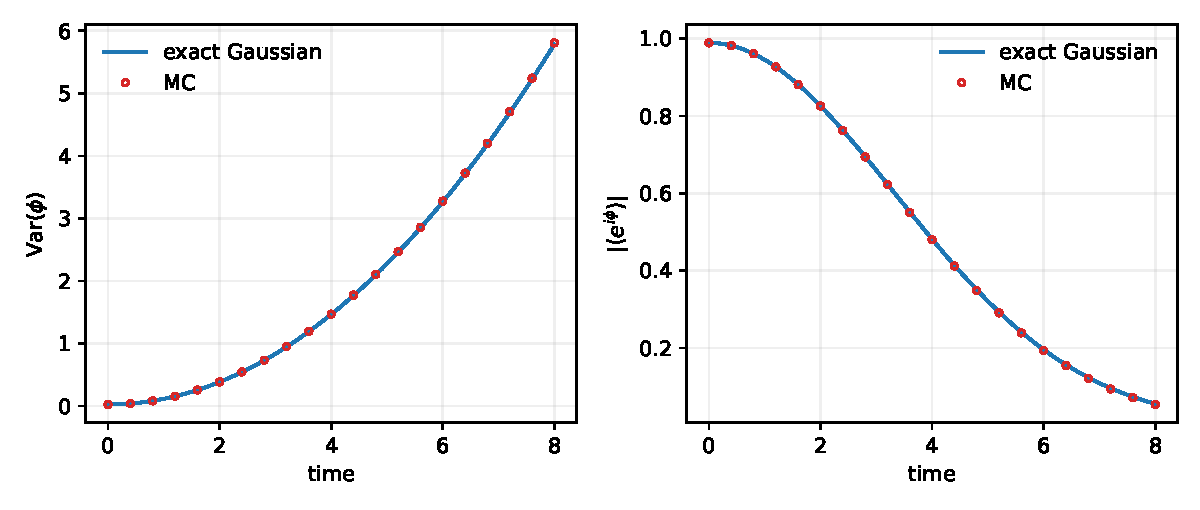
\includegraphics[width=0.78\textwidth]{figures/ch16/phase_diffusion.pdf}
  \caption[相对相位扩散的高斯 Monte Carlo 基准]{相对相位扩散的解析式与 Monte Carlo 对照。参数为 $E_C=0.1$、$\sigma_N=3$、$\sigma_\phi=0.15$，点和 $\pm1$ 标准误来自 $200000$ 条高斯轨迹；相位方差与相干包络的最大偏差分别为 $1.36$、$1.51$ 个标准误以内。该图只检验可逆零模剪切，不含空间传播、碰撞或耗散。}
  \label{fig:phase-diffusion-benchmark}
\end{figure}
图中相干衰减完全来自相对数导致的可逆相空间剪切，没有加入碰撞或耗散。指标保存在
\path{data/ch16/phase_diffusion_metrics.json}。

\section{端到端空间场淬火基准}

前一个基准只检验零模解析公式。为把第10--15章的环节真正接起来，配套程序
\path{code/ch14_17_capstone/two_component_field_quench.py}
执行一次受限但完整的双分量空间场计算：在 $\hbar=m=1$ 的单位中取周期长度 $L=32$、$64$ 个格点、凝聚背景总密度参数 $n=12$、$g=0.05$、$g_{12}=0.035$、$T=0.30$，先在 $J_i=0.15$ 的稳定密度/自旋 BdG 基中抽样有限温 Wigner 噪声，再突然关闭均匀 Rabi 耦合到 $J_f=0$，最后用含 Weyl 基线的双分量 Strang 分步法传播。这里 $n$ 是展开点的凝聚背景密度，$nL=384$ 不是抽样后的正规排序总粒子数；后者的系综均值为 $406.83$，还包含该有限 BdG 基中的量子与热耗尽。

密度 $k=0$ 是 Goldstone 坐标，不能代入普通热 BdG 振子公式。这里把它定义成承载宏观位移的凝聚相干零模，并抽样其真空 Wigner 噪声，即 $\ensavg{|b_{d,0}|^2}=1/2$、$\ensavg{b_{d,0}^2}=0$，但不赋予热 BdG 占据；有隙自旋零模则仍按有限温 BdG 协方差抽样。因此密度/自旋两个通道的全部 $2N_x$ 个模式都各自带有相应的 Wigner 半量子，与排序基线所计数的 $2N_x$ 个正则原子模式逐一对应。这个方案并不固定总粒子数：宏观零模的真空噪声会产生真实的样本间总数涨落，不能再称作数守恒抽样；本次初态正规排序总数在 $256$ 个样本间的标准差为 $26.67$，即均值的 $6.56\%$（其中也含其余密度模的量子与热涨落）。程序逐模检查 $b_k$ 的正常矩与 $b_kb_{-k}$ 反常矩，并在变换到原子密度/自旋通道后再次检查目标协方差；本次最大标准化残差分别为 $3.65$ 和 $3.66$，均低于预先写入指标文件的 $5$ 标准误门槛。Fourier 完备性、通道幺正性和 BdG 辛归一化的最大代数残差为 $3.7\times10^{-15}$。

观测量不是逐轨迹归一化后再平均，而是式\eqref{eq:intercomponent-coherence}对应的比值--系综估计器
\begin{equation}
  C_{LR}^{\rm est}(t)=
  \frac{\ensavg{\int\dd x\,\psi_L^*(x,t)\psi_R(x,t)}}
  {\sqrt{\ensavg{N_{L,W}}\ensavg{N_{R,W}}}},
  \qquad
  N_{\sigma,W}=\int\dd x\left(|\psi_\sigma|^2-\frac12\delta_{\mathcal C}\right).
  \label{eq:capstone-coherence-estimator}
\end{equation}
同时计算最低非零波矢 $k_1=2\pi/L$ 的正规排序自旋结构因子。这里两个
分量共有 $2N_x$ 个正则格点模式，故原始对称范数与数算符 Weyl 符号的关系是
\begin{equation}
  \mathcal N_{\mathrm{sym}}^{(s)}=\Delta x\sum_j
  (|\psi_{L,j}^{(s)}|^2+|\psi_{R,j}^{(s)}|^2),
  \qquad
  N_W^{(s)}=\mathcal N_{\mathrm{sym}}^{(s)}-N_x.
  \label{eq:capstone-number-symbol}
\end{equation}
关闭耦合后，程序还直接计算与同一有限格点基一致的离散 Weyl 哈密顿量
\begin{align}
  H_W={}&\sum_k\epsilon_k
  \left(|a_{L,k}|^2+|a_{R,k}|^2-1\right) \notag\\
  &+\frac{g\Delta x}{2}\sum_j\left[
  n_{L,j}^2+n_{R,j}^2-2\delta_{\mathcal C}(n_{L,j}+n_{R,j})
  +\delta_{\mathcal C}^2\right] \notag\\
  &+g_{12}\Delta x\sum_j
  \left(n_{L,j}-\frac{\delta_{\mathcal C}}2\right)
  \left(n_{R,j}-\frac{\delta_{\mathcal C}}2\right),
  \qquad n_{\sigma,j}=|\psi_{\sigma,j}|^2,
  \label{eq:capstone-discrete-weyl-hamiltonian}
\end{align}
其中 $a_{\sigma,k}$ 采用与实空间格点正交归一的 Fourier 约定，且
$\delta_{\mathcal C}=1/\Delta x$。动能中的 $-1$ 正是两个分量各自的半量子；相互作用项的线性项与常数项也不能遗漏，否则“能量守恒”检查的对象就不是实际传播的 Weyl 哈密顿量。
对同一完整正交格点基，结构因子的乘积估计器要扣除 $N_x/2$：
\begin{equation}
  S_s(k_1)=\frac{\ensavg{|S_{k_1,W}|^2}-N_x/2}{\ensavg{N_W}},
  \qquad
  S_{k,W}=\Delta x\sum_j\ee^{-\ii kx_j}
  (|\psi_{L,j}|^2-|\psi_{R,j}|^2).
  \label{eq:capstone-spin-structure-estimator}
\end{equation}

完整结果汇总于\cref{fig:two-component-field-capstone}。
\begin{figure}[htbp]
  \centering
  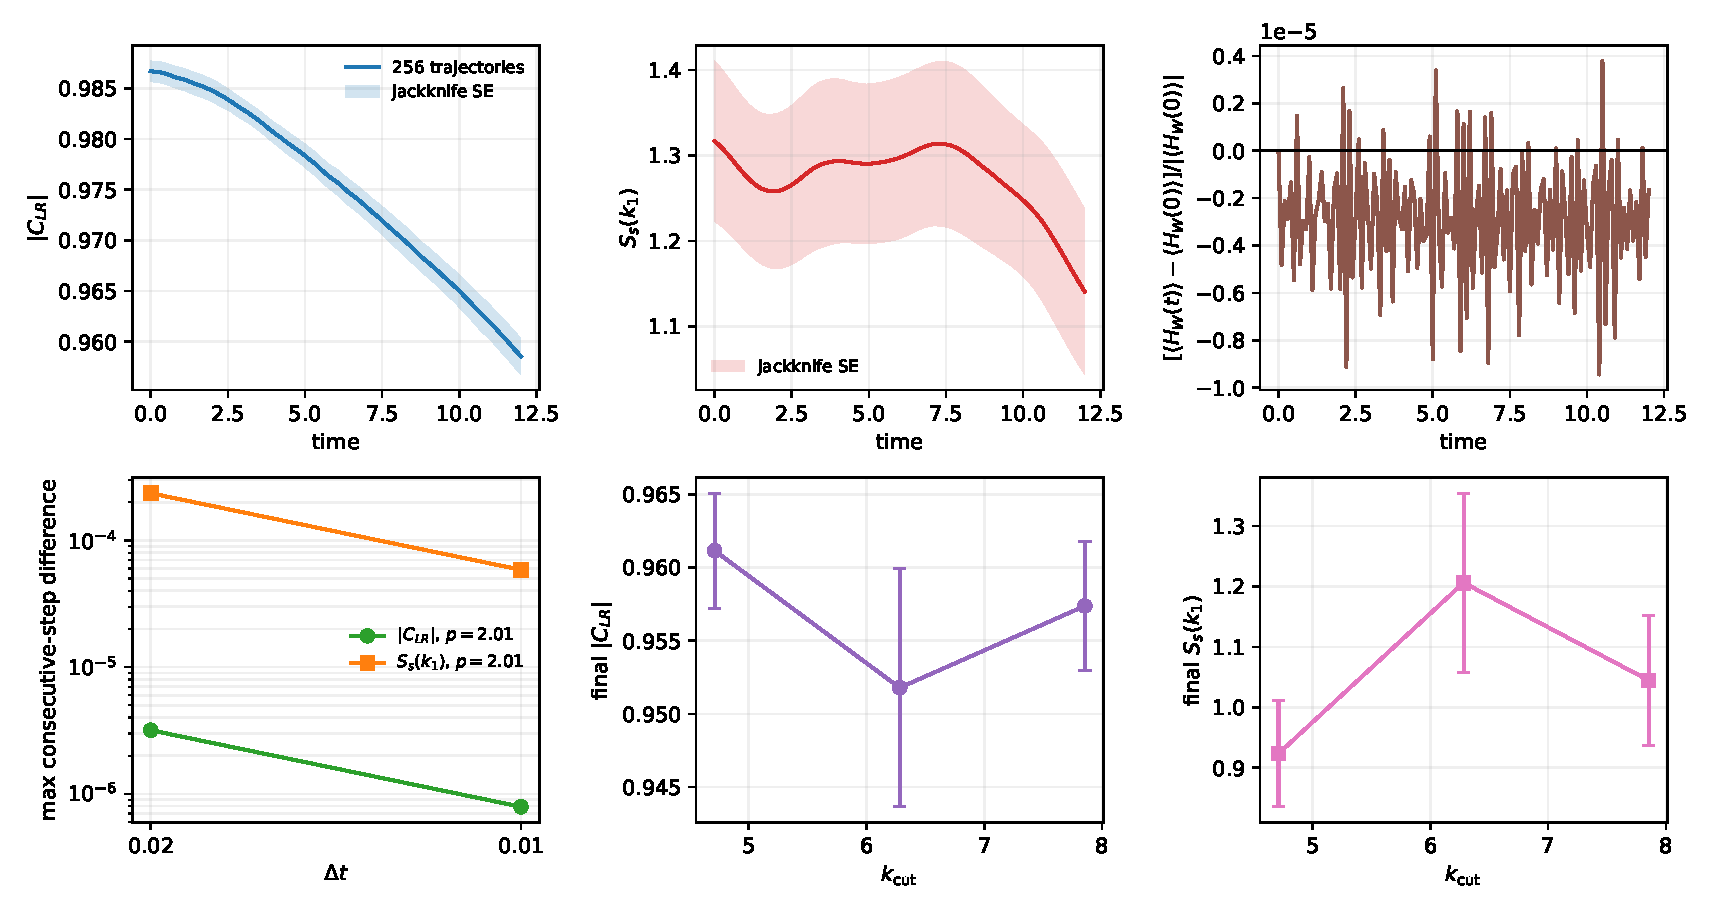
\includegraphics[width=0.96\textwidth]{figures/ch14_17_capstone/two_component_field_quench.pdf}
  \caption[双分量空间场淬火的端到端基准]{均匀 Rabi 双分量场从 $J_i=0.15$ 淬火到 $J_f=0$ 的端到端基准。生产曲线使用 $L=32$、$N_x=64$、$256$ 条轨迹，阴影为 $\pm1$ 删除分块 jackknife 标准误；其余面板显示离散 Weyl 能量漂移、$\Delta t=0.02,0.01,0.005$ 的二阶标度，以及 $N_x=48,64,80$ 截止压力测试（每档64条独立轨迹，误差棒为 $\pm1$ 标准误）。抽样的128个通道模式与排序基线一致，20项机器门禁全部通过。该结果只支持所测试有限时间和截止窗内的空间去相位与估计器闭环，不是 Raman SOC、预热化平台、热化或网格极限的证据。}
  \label{fig:two-component-field-capstone}
\end{figure}
在 $256$ 条轨迹中，$|C_{LR}|$ 从 $0.9867$ 降到 $0.9586$。相干曲线的删除分块 jackknife 标准误最大为 $1.79\times10^{-3}$，所以这一下降在本样本中清楚可分辨。最低非零波矢的 $S_s(k_1)$ 从 $1.317$ 变到 $1.141$，但它的全曲线 jackknife 标准误最大为 $0.098$；图中的误差带表明，当前轨迹数还不足以把每个细小振荡都解释成确定的空间模式信号。因而 $S_s(k_1)$ 在这里首先是排序修正与不确定度传播的实际场估计器验收，而不是独立的预热化证据。

用相同初态噪声比较 $\Delta t=0.02,0.01,0.005$，相干与 $S_s(k_1)$ 的连续差分都给出 Strang 观测阶 $2.01$；最细两档的最大曲线差分别为 $7.91\times10^{-7}$ 和 $5.86\times10^{-5}$，远小于相应 Monte Carlo 误差。把轨迹数从 $256$ 降至 $128$ 时，两条曲线的最大变化分别相当于 $1.29$ 和 $1.56$ 个 $256$ 轨迹最大 jackknife 标准误。总物理粒子数最大相对漂移为 $1.01\times10^{-13}$。式\eqref{eq:capstone-discrete-weyl-hamiltonian}的系综平均相对漂移不超过 $9.44\times10^{-6}$，单轨迹漂移的均方根不超过 $8.42\times10^{-5}$；共同噪声下每次把步长减半，系综能量漂移分别缩小到前一档的 $0.246$ 和 $0.249$，与二阶分步误差一致。

程序还在同一 $L$ 和已验收的 $\Delta t=0.005$ 下，对 $N_x=48,64,80$ 三个模式截止各自独立重新抽样 $64$ 条轨迹。终态相干分别为 $0.9611\pm0.0039$、$0.9518\pm0.0081$ 和 $0.9574\pm0.0044$，最大两两差异为 $1.04$ 个合并标准误；终态 $S_s(k_1)$ 分别为 $0.923\pm0.088$、$1.206\pm0.148$ 和 $1.045\pm0.108$，最大两两差异为 $1.64$ 个合并标准误。三档的系综平均 Weyl 能量最大相对漂移均不超过 $1.37\times10^{-5}$。由于三档数据不是嵌套样本、统计精度有限且没有显示单调趋势，这只是给定有限截止窗内未检出显著差异的压力测试，不能称作网格极限收敛。完整曲线、参数、随机种子、逐模矩、零模处理清单、结构化阈值与验收结果和截止数据保存在
\path{data/ch14_17_capstone/two_component_field_quench_metrics.json}。

这个结果只支持“在已测试的有限截止窗和有限时间内观察到空间场去相位”的结论。它没有做高精度截止外推和系统尺寸扫描，也没有展示随时间演化的模式占据在平台内保持、随后碰撞再分配，因此\emph{不是}预热化平台、更不是量子热化的证据；它也使用均匀 Rabi 模型而非 Raman SOC。初态的逐模正常矩与反常矩在这里只是抽样门禁，不能替代上述动力学证据。要把结论升级为预热化，至少还要输出这些矩的时间序列，识别式\eqref{eq:prethermal-window}的时间尺度分离，并扩大截止与尺寸扫描。

\section{从轨迹提取相对相位}

低密度点的局域相位噪声会发散，直接平均
$\arg\psi_R(x)-\arg\psi_L(x)$ 不稳健。全局相位可由复重叠
\begin{equation}
  A_{LR}^{(s)}(t)=\int\dd x\,
  \psi_L^{(s)*}(x,t)\psi_R^{(s)}(x,t),
  \qquad
  \phi_s=\arg A_{LR}^{(s)}
  \label{eq:trajectory-relative-phase}
\end{equation}
定义，并用圆统计量
\begin{equation}
  R_\phi=\left|\frac1{N_s}\sum_s\ee^{\ii\phi_s}\right|
  \label{eq:circular-resultant}
\end{equation}
衡量相位锁定。均匀分布在有限样本下也给出正的 $R_\phi$，应通过随机均匀相位空模型或已知的圆统计分布校准，而不是把任何非零值解释为残余相干。

\begin{chaptercheck}
当相干因子下降时，同时画出：相对相位圆分布、零模相对数、各 $k$ 正常占据、反常关联、总能量和反向传播误差。只有这些量的联合变化才能区分相位扩散、线性去相位、非线性再分配和数值伪阻尼。
\end{chaptercheck}

\section*{本章小结}

全局相位扩散由相对数不确定度造成，高斯相干包络可由协方差精确预测；空间模式的线性去相位可以产生预热化平台，却不改变二次理论中的模式占据。非线性场方程包含模式耦合，但 TWA 晚时阻尼仍可能是可逆混合或截止相关经典化。碰撞热化与不可逆性需要回波、占据再分配、分布和独立量子方法共同支持。

\begin{exercises}
  \item 从式\eqref{eq:phase-diffusion-trajectory}推导含非零初始交叉协方差的式\eqref{eq:phase-variance-growth}。
  \item 对精确固定相对数态解释为什么不能同时指定一条确定初始相位轨迹；再说明窄数压缩波包何时可近似使用高斯相位扩散公式。
  \item 在二次模式理论中证明正常模式占据不变而反常矩发生相位旋转。
  \item 设计一个回波协议，分别对纯去相位与弱碰撞情形给出预期结果。
  \item 提出至少三项证据，区分 Bose--Einstein 热分布与截止相关 Rayleigh--Jeans 分布。
  \item 扩展端到端空间场程序，输出淬火后密度/自旋 BdG 模的正常占据和反常矩，并据此检验是否存在式\eqref{eq:prethermal-window}，而不是仅凭 $C_{LR}(t)$ 命名预热化。
\end{exercises}

\chapter{条纹序、有限尺寸与超固态判据}
\label{ch:order-diagnostics}

\begin{learningobjectives}
完成本章后，读者应能：
\begin{enumerate}
  \item 用对称性不变的结构因子和有限尺寸标度诊断条纹长程序；
  \item 区分密度调制、相分离、显式钉扎与自发平移对称破缺；
  \item 为超固态结论同时检验密度序和超流响应；
  \item 对一维、有限温、非平衡和 TWA 晚时结果使用与证据相称的结论措辞。
\end{enumerate}
\end{learningobjectives}

\section{“有条纹”还不是超固态}

超固态的核心是两类性质共存\cite{Boninsegni2012}：
\begin{enumerate}
  \item 与平移对称破缺相关的晶体或密度波有序；
  \item 与全局 $U(1)$ 相位刚度相关的超流响应。
\end{enumerate}
一张单轨迹密度图出现周期起伏，只满足了最弱的候选信号。相分离后的畴壁、动力学不稳定的最快增长模、外势直接压出的密度波和有限采样噪声都能产生类似图样。反过来，对称性未显式破缺的有限系统中，系综平均密度可以完全均匀，而密度关联仍含有长程序。

因此本章不从“对比度是否非零”直接裁决超固态，而建立一组顺序明确的检验。

\section{条纹序参量与结构因子}

对长度 $L$ 的双分量 TWA 场，先定义正规排序总密度的单轨迹 Wigner 符号及其 Fourier 分量
\begin{equation}
  \begin{aligned}
  n_W^{(s)}(x)&=\sum_{\sigma=L,R}
  \left(|\psi_\sigma^{(s)}(x)|^2-\frac12\delta_{\mathcal C}(x,x)\right),\\
  M_Q^{(s)}&=\int_0^L\dd x\,\ee^{-\ii Qx}n_W^{(s)}(x),
  &N_W^{(s)}&=M_0^{(s)}.
  \end{aligned}
  \label{eq:trajectory-stripe-fourier-symbol}
\end{equation}
上标 $s$ 只是抽样轨迹编号，不代表一次物理单次测量；特别是低占据时，$N_W^{(s)}$ 可以有很大噪声，局部 $n_W^{(s)}$ 甚至可以为负。因此不应默认先形成随机比值 $M_Q^{(s)}/N_W^{(s)}$ 再平均。令 $\bar N=\ensavg{N_W}$，推荐使用比值--系综估计器
\begin{equation}
  \bar m_Q=\frac{\ensavg{M_Q}}{\bar N},
  \qquad
  \mathcal M_Q^2=
  \frac{\ensavg{|M_Q|^2}-C_Q^{(W)}}{\bar N^2}.
  \label{eq:ensemble-stripe-estimators}
\end{equation}
这里 $N_W^{(s)}=(\hat N)_W$ 已含每模半量子扣除；未扣除的原始模方和统一
记作 $\mathcal N_{\mathrm{sym}}^{(s)}$，两者不得互换。
第一项保留条纹平移相位，第二项是对称性不变的强度。若物理总粒子数在每个样本中被严格固定为同一个 $N$，才可等价地用固定分母 $M_Q^{(s)}/N$。

$C_Q^{(W)}$ 是\emph{双线性乘积}的 Weyl 接触修正，不能因 $Q\neq0$ 就遗漏。若 $M_Q$ 在保留的单粒子基中对应矩阵 $A_Q$，并且所选离散表示满足 $[A_Q,A_{-Q}]=0$，则
\begin{equation}
  C_Q^{(W)}=\frac14\Tr_{\mathcal C,\sigma}(A_QA_{-Q}).
  \label{eq:stripe-product-weyl-contact}
\end{equation}
在两个分量、$N_x$ 点的正交 collocation 格点且 $A_Q$ 只是格点相位时，$C_Q^{(W)}=N_x/2$。若先做谱投影再乘密度相位，截止边界可能使 $A_Q$ 与 $A_{-Q}$ 不对易；此时应直接计算该有限基中的完整星积，不能只套用式\eqref{eq:stripe-product-weyl-contact}的常数项。这个修正对宏观 Bragg 峰不改变热力学指数，却会污染低占据、小系统和无序基线。

无外场时，不同轨迹可以选择不同条纹原点，使
\begin{equation}
  \bar m_Q=0,
  \qquad
  \mathcal M_Q^2>0.
  \label{eq:symmetry-restored-stripe-ensemble}
\end{equation}
所以只看平均密度会漏检对称性恢复系综中的关联序。与第13章结构因子相连，在忽略不影响标度的规范差异时，Bragg 峰满足
\begin{equation}
  S_{\rm tot}(Q)=\frac{\ensavg{|M_Q|^2}-C_Q^{(W)}}{\bar N}
  =\bar N\mathcal M_Q^2,
  \qquad
  S_{\rm conn}(Q)=S_{\rm tot}(Q)-\bar N|\bar m_Q|^2.
  \label{eq:bragg-order-scaling}
\end{equation}
$S_{\rm tot}$ 保留显式钉扎或有限对称破缺场的弹性峰，$S_{\rm conn}$ 则扣掉平均密度调制。报告时必须说明采用哪一个。

固定密度取 $L,N\to\infty$ 时，三类标度可作初步区分：
\begin{center}
\begin{tabularx}{\textwidth}{p{0.25\textwidth}XX}
\toprule
密度关联 & $\mathcal M_Q^2$ & $S_{\rm tot}(Q)$ \\
\midrule
真正长程序 & 趋于非零常数 & 与 $N$ 成正比 \\
准长程序，$0<\eta<1$ & 约为 $L^{-\eta}$ & 约为 $L^{1-\eta}$ \\
有限关联长度 & 约为 $L^{-1}$ & 趋于常数量级 \\
\bottomrule
\end{tabularx}
\end{center}
这里假定振荡关联包络 $C_Q(r)\sim r^{-\eta}$。$\eta=0$ 对应真正长程序；$0<\eta<1$ 时积分给出上表幂律；$\eta=1$ 可出现对数修正；$\eta>1$ 时 $S(Q)$ 的领先项已为常数量级，仅靠该峰的幂指数不能再与有限关联长度区分。不能用单一尺寸区分这些情况。拟合时应比较“常数加有限尺寸修正”、幂律和有限相关长度模型，而不是预先选定最想看到的一个。

\section{波矢选择与峰值偏差}

目标 $Q$ 应优先由单粒子带极小值、Bogoliubov 软模或独立实验标定给出。若每条轨迹都在宽波数窗内寻找最大峰，再把最大值平均，即使无序噪声也会得到正偏差。可采用：
\begin{enumerate}
  \item 在独立训练数据上确定 $Q$ 和积分窗，在测试数据上估计强度；
  \item 对预注册的固定波数窗积分 Bragg 权重；
  \item 把完整寻峰算法应用到无序空模型，校准选择偏差；
  \item 在改变 $L$ 时保持物理波数窗，而不是保持固定 FFT 格点数。
\end{enumerate}

有限系统允许的离散波数可能不恰好包含理论 $Q$。应使用与边界相容的尺寸序列、扭曲边界或窗函数，并量化谱泄漏。把不同尺寸的最近 FFT 格点直接比较会把失配误判成序参量衰减。

\section{显式钉扎与自发破缺}

若哈密顿量含有 $h\cos(Qx)\hat n(x)$ 的外势，密度在有限 $h$ 下调制是显式响应。自发破缺的热力学定义要求按顺序取极限
\begin{equation}
  m_Q^{\rm SSB}=\lim_{h\to0^+}\lim_{L\to\infty}\qavg{m_Q}_{L,h}.
  \label{eq:ssb-order-of-limits}
\end{equation}
这里 $m_Q$ 表示正规排序密度算符除以物理 $N$，不是式\eqref{eq:trajectory-stripe-fourier-symbol}的单轨迹随机比值。有限尺寸、严格 $h=0$ 的精确本征态通常保持对称，故 $\qavg{m_Q}=0$ 并不排除热力学有序；有限 $h$ 下 $m_Q\neq0$ 也不证明自发有序。实际计算可结合零场 $\mathcal M_Q^2$ 标度、弱钉扎场响应和极限顺序。

Raman 光决定反冲波数，却未必等价于直接的密度晶格势。需要从实验室表象的完整哈密顿量判断条纹平移相位是自由集体坐标、只剩离散选择，还是已经被外场唯一钉扎。自旋轨道耦合凝聚体中“具有超固态性质的条纹相”已有实验实现\cite{Li2017}，但具体模型的对称性与诊断仍须逐项核对。

\section{超流性的独立检验}

密度序只是超固态的一半。对两个分量施加相同的边界扭转
\begin{equation}
  \psi_{L,R}(x+L)=\ee^{\ii\Theta}\psi_{L,R}(x),
  \label{eq:common-phase-twist-boundary}
\end{equation}
检验的是总质量 $U(1)$ 的相位刚度；相反扭转 $\Theta_L=-\Theta_R$ 检验的是自旋或相对相位刚度，二者不能互换。对一维平衡体系先定义无歧义的 helicity modulus
\begin{equation}
  \Upsilon=L\left.\frac{\partial^2F(\Theta)}{\partial\Theta^2}\right|_{\Theta=0},
  \label{eq:helicity-modulus-twist}
\end{equation}
其中零温时 $F$ 可换成基态能 $E$。只有在单一裸质量 $m$、普通 Galilean 归一化适用时，才进一步定义无量纲超流分数
\begin{equation}
  f_s=\frac{mL^2}{N\hbar^2}
  \left.\frac{\partial^2F(\Theta)}{\partial\Theta^2}\right|_{\Theta=0}.
  \label{eq:superfluid-fraction-twist}
\end{equation}
对 Galilean 不变、零温且完全超流的均匀体系，
$E(\Theta)-E(0)=N\hbar^2\Theta^2/(2mL^2)$，故 $f_s=1$。实际有限差分应成对计算
\begin{equation}
  F''(0)\simeq\frac{F(+\Theta)+F(-\Theta)-2F(0)}{\Theta^2},
  \label{eq:twist-central-difference}
\end{equation}
并扫描 $\Theta$ 以排除非线性响应。SOC 破坏普通 Galilean 不变性，响应可以是方向相关的张量，且用裸质量归一化出的量未必仍是 $[0,1]$ 内的“分数”；此时应优先报告共同规范扭转下的 $\Upsilon$ 或完整响应张量。规范表象中的扭转还要与 Raman 边界条件一致，不能只把 FFT 动量整体平移而保持激光相位约定不变。

其他互补指标包括：
\begin{enumerate}
  \item 一体密度矩阵最大本征值及 $g^{(1)}(r)$ 的长距离标度；
  \item 对弱矢势、缓慢移动边界或微小流速的线性电流响应；
  \item 平衡路径积分中的绕数涨落；
  \item 持久流稳定性与声学 Goldstone 响应。
\end{enumerate}
有限系统中宏观占据一个轨道不等于热力学超流刚度；反之，一维体系可以没有真正凝聚分数却保持有限相位刚度。应选择与维数、平衡/非平衡状态和可用方法相符的指标。

TWA 时间轨迹不能直接给出热力学自由能曲率。可在同一初态系综上施加成对的微小正负规范扭转或矢势，测量线性电流响应；若要声称平衡超流分数，还需证明所取状态和响应协议对应适当系综，并检查扰动幅度与等待时间极限。

\section{一维和有限温的限制}

在短程相互作用的一维体系中，连续对称性的涨落格外强。Hohenberg 定理排除热力学极限下有限温连续对称性的常规长程序\cite{Hohenberg1967}。零温低能区通常由 Luttinger 液体描述，相位和密度关联呈参数依赖的幂律\cite{Haldane1981,Cazalilla2004}；相应的密度波峰可以是代数奇点，而不是与体积成正比的真正 Bragg 峰。长程相互作用、晶格、显式钉扎或有限横向尺寸会改变结论，因此任何外推都必须重新检查理论前提。

因此，对准一维有限管中的“超固态”更稳健的表述可能是：在给定长度和时间窗内，观察到密度波关联与超流响应共存；其向热力学、长时间和严格一维极限的外推仍需标度。若只得到幂律密度序与幂律一体相干，可称为准长程序共存，而不宜无条件宣称严格长程超固态。

\section{淬火后条纹不是自动的平衡相}

淬火可以选择最快增长波矢并产生长寿命图样，但该图样可能是：
\begin{enumerate}
  \item 线性不稳定后的畴结构；
  \item 预热化平台中的准稳态关联；
  \item 守恒量约束下的非热稳态；
  \item 最终平衡有序相的早期成核；
  \item 截止相关经典场热化的暂态。
\end{enumerate}
要称为平衡超固态，需要在给定能量/温度和粒子数下独立建立平衡性。若只研究有限时间非平衡动力学，应使用“瞬态条纹序”“预热化密度波”或“超固态样共存”等更准确措辞。

相对相位在 $[0,2\pi)$ 上均匀也不能单独裁决。它可能意味着跨分量一阶相干消失；若 $M_Q^{(s)}$ 的相位跨轨迹随机而正规修正后的 $\mathcal M_Q^2$ 随尺寸保持，它也可能只是对称性恢复系综中条纹位置随机。反之，如果 $\mathcal M_Q^2\sim1/L$，才支持有限相关长度。必须把相位分布与幅度标度结合。

\section{一致的有限尺寸协议}

对 TWA 尺寸标度，建议保持以下物理量不变：
\begin{enumerate}
  \item 平均密度、相互作用常数、温度或单位粒子注入能；
  \item 物理格距或能量截止，而非格点总数；
  \item 边界条件、Raman 参数和目标 $Q$ 的物理窗口；
  \item 观测时间的物理定义，例如以声速穿越时间或碰撞时间归一；
  \item 每个尺寸下足以分辨 $S_{\rm tot}(Q)\sim N$ 与 $S_{\rm tot}(Q)\sim1$ 的轨迹数。
\end{enumerate}
固定密度和截止时，$N$ 与保留模式数 $M$ 都随 $L$ 增大，半量子总量也广延增长。这正是需要重复第9章截止稳定检查的原因。

推荐的判据矩阵如下：
\begin{center}
\begin{tabularx}{\textwidth}{p{0.22\textwidth}XX}
\toprule
主张 & 最低证据 & 关键反例排除 \\
\midrule
存在条纹关联 & $S_{\rm tot}(Q)$ 峰及实空间关联 & FFT 泄漏、寻峰偏差、外势 \\
长程密度序 & $S_{\rm tot}(Q)\propto N$ 或 $\mathcal M_Q^2\to c>0$ & 有限相关长度、畴平均 \\
存在超流性 & 扭转曲率或线性流响应 & 仅有凝聚峰、有限时间惯性 \\
超固态共存 & 同一状态中前两类证据同时成立 & 不同时间窗或不同参数拼接 \\
平衡自发破缺 & 尺寸、钉扎场和长时间极限 & 显式驱动、预热化暂态 \\
\bottomrule
\end{tabularx}
\end{center}

\section{实际随机相位标度基准}

配套程序生成两个明确的统计玩具模型，而不冒充完整凝聚体动力学：其一是整条系统具有随机全局条纹相位的有序系综，其二是固定相关长度的独立相位畴系综。所有密度场均由程序实际生成，结果见\cref{fig:stripe-scaling-toy}。
\begin{figure}[htbp]
  \centering
  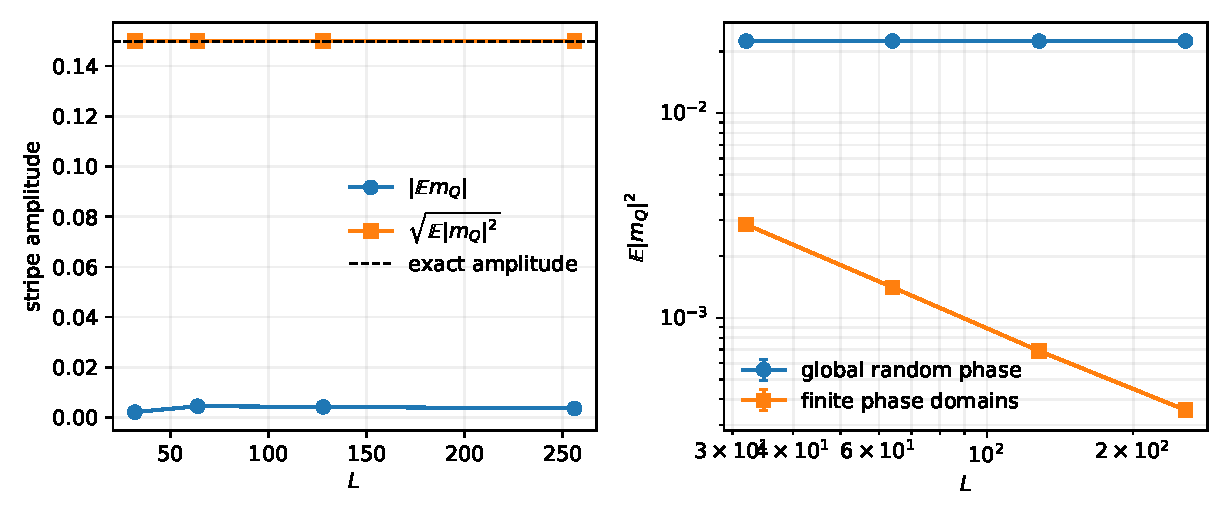
\includegraphics[width=0.78\textwidth]{figures/ch17/stripe_scaling_toy.pdf}
  \caption[条纹序有限尺寸标度的统计玩具模型]{条纹序有限尺寸标度的统计玩具模型。对 $L=32,64,128,256$，每个长度独立生成 $2000$ 条密度轨迹；右图误差棒为 $\pm1$ 标准误。随机全局相位系综的 $\mathcal M_Q^2$ 斜率在数值精度内为零，固定长度相位畴系综的对数斜率为 $-1.007\pm0.011$。该图演示“均值为零不等于无序”和有限尺寸判据，不是相互作用量子场的动力学证据。}
  \label{fig:stripe-scaling-toy}
\end{figure}
前者满足 $|\bar m_Q|\simeq0$ 但
$\mathcal M_Q^2$ 趋于常数；后者随 $L^{-1}$ 衰减。这个高占据经典玩具模型的程序变量沿用旧名 \texttt{m\_Q}，没有加入式\eqref{eq:stripe-product-weyl-contact}的量子接触项；将其迁移到 TWA 数据时必须加入该项。数据和拟合斜率保存在
\path{data/ch17/stripe_scaling_toy_metrics.json}。该基准只验证分析管线，不是本书对具体 Raman 参数下超固态的数值宣判。

\begin{chaptercheck}
只有当同一组参数和同一状态同时通过密度序标度、超流响应、显式钉扎排除、截止/步长/轨迹收敛和 TWA 有效时间检查，才把结论提升为“受 TWA 支持的超固态候选”。若还缺独立量子方法或平衡性证据，应把这些限制写进结论句本身。
\end{chaptercheck}

\section*{本章小结}

随机条纹相位会令平均密度均匀，却不抹去对称性不变的 Bragg 关联；真正长程序必须由 $S_{\rm tot}(Q)$ 或 $\mathcal M_Q^2$ 的尺寸标度识别。超固态还要求同一状态具有独立的共同 $U(1)$ 相位刚度。显式钉扎、一维涨落、非平衡暂态和 TWA 晚时截止效应都会降低可作结论的强度。相位均匀、条纹对比度下降或单尺寸 Bragg 峰都不能单独完成“自发对称破缺”的裁决。

\begin{exercises}
  \item 考虑随机全局相位的密度
  \[
    n(x)=n_0[1+A\cos(Qx+\theta)].
  \]
  计算 $\bar m_Q$ 与 $\mathcal M_Q^2$；在经典连续密度模型中取 $C_Q^{(W)}=0$。
  \item 设系统由 $L/\xi$ 个独立相位畴组成，推导 $\mathcal M_Q^2\propto\xi/L$。
  \item 从两个分量、$N_x$ 个格点模式的 Weyl 星积推导 $C_Q^{(W)}=N_x/2$，并估计遗漏该项对低占据 $S_{\rm tot}(Q)$ 的偏差。
  \item 验证式\eqref{eq:superfluid-fraction-twist}对均匀完全超流给出 $f_s=1$。
  \item 对 $C_Q(r)\sim\cos(Qr)r^{-\eta}$ 分别推导 $0<\eta<1$、$\eta=1$ 和 $\eta>1$ 时的有限尺寸标度。
  \item 设计尺寸与弱钉扎场的二维外推，以实现式\eqref{eq:ssb-order-of-limits}。
  \item 为“淬火后形成平衡超固态”列出一条可能否定该命题的最小数值结果。
\end{exercises}


\part{方法边界与扩展}
\chapter{开放系统、替代方法与研究工作流}
\label{ch:extensions-workflow}

\begin{learningobjectives}
完成本章后，读者应能：
\begin{enumerate}
  \item 从 Lindblad 主方程识别 Wigner 漂移、扩散与额外截断；
  \item 根据初态、维数、占据、观测量和时间尺度选择 TWA 或替代方法；
  \item 把物理主张转化为带基准、收敛、元数据和停止条件的计算工作流；
  \item 为可复现研究保存从输入、代码、随机数到最终图表的证据链。
\end{enumerate}
\end{learningobjectives}

\section{开放系统的相空间方程}

Markov 开放系统常写成 Lindblad 方程\cite{Lindblad1976}
\begin{equation}
  \partial_t\rhohat=-\frac{\ii}{\hbar}\comm{\Hhat}{\rhohat}
  +\sum_\ell\left(
  \hat L_\ell\rhohat\hat L_\ell^\dagger
  -\frac12\acomm{\hat L_\ell^\dagger\hat L_\ell}{\rhohat}
  \right).
  \label{eq:lindblad-master-equation}
\end{equation}
Wigner 变换后，线性 Lindblad 算符通常产生至多二阶导数，得到真正的 Fokker--Planck 方程。以单模损耗
$\hat L=\sqrt\kappa\,\ha$ 为例，在复 Wiener 增量满足
$\ensavg{\dd W\dd W^*}=\dd t$、$\ensavg{\dd W^2}=0$ 的约定下，轨迹为
\begin{equation}
  \dd\alpha=\left[-\frac{\ii}{\hbar}
  \frac{\partial H_W}{\partial\alpha^*}
  -\frac\kappa2\alpha\right]\dd t
  +\sqrt{\frac\kappa2}\,\dd W.
  \label{eq:wigner-linear-loss-sde}
\end{equation}
噪声项不是数值误差，而是保持真空涨落所必需的扩散。若只给经典场加阻尼而不加相应噪声，会破坏量子稳态和涨落--耗散关系。

非线性跳跃算符或非线性 Hamilton 量仍可能产生三阶及更高导数。此时把方程截为二阶是开放系统 TWA，既含 Hamilton 截断误差，也可能含耗散通道截断误差。还必须声明随机微分方程采用 It\^o 还是 Stratonovich 解释；两者漂移在乘性噪声下不同。

\section{TWA 之外的相空间方法}

\subsection{positive-P 表示}

positive-P 把每个模式扩充为独立复变量 $\alpha,\beta$，不要求
$\beta=\alpha^*$。对许多最多四次的玻色 Hamilton 量，主方程可精确映射为二阶 Fokker--Planck 方程，因此原则上没有 TWA 的 Moyal 截断。代价是轨迹权重和变量可能形成长尾，抽样方差随时间爆炸，边界项也需诊断。它是“动力学表示更精确但统计窗口可能更短”的方法，而不是无条件优于 TWA。
这一加倍相空间构造的经典来源见文献\cite{Drummond1980}。

\subsection{随机规范与混合表示}

gauge-P 等方法通过附加权重和随机规范改变扩散路径，尝试延长可用时间；选择不当会带来权重离群和偏差。不同模式也可采用混合表示，例如高占据凝聚模用 Wigner、低占据量子模用正 P，但跨表示耦合必须从统一主方程推导。

\subsection{Husimi Q 与 Glauber--Sudarshan P}

Q 函数总为非负，却对应反正规排序，动力学方程未必易于抽样；传统 P 表示对应正规排序，但对非经典态可能比普通函数更奇异。相空间分布的正性、算符排序便利和动力学阶数是三项不同属性，不能只按“是否能画成概率密度”选方法。

\section{非相空间替代方法}

\begin{center}
\begin{tabularx}{\textwidth}{>{\raggedright\arraybackslash}p{0.20\textwidth}>{\raggedright\arraybackslash}X>{\raggedright\arraybackslash}X}
\toprule
方法 & 强项 & 主要限制与交叉用途 \\
\midrule
精确对角化 & 小系统全量子谱与任意观测量 & Hilbert 空间指数增长；用于少模、低粒子数、短时基准 \\
MPS/张量网络\cite{Vidal2003} & 一维局域模型、受控截断 & 纠缠增长限制长时与高维；用于一维短中时关联 \\
量子蒙特卡洛 & 平衡态、无符号问题时高精度 & 实时与符号问题；用于平衡能量、刚度、结构因子 \\
Bogoliubov 法 & 弱涨落、解析协方差 & 非线性饱和不足；用于早时、稳定谱和软模 \\
Keldysh 动理学 & 弱耦合长时碰撞与输运 & 依赖闭合和梯度展开；用于模式占据与碰撞率 \\
正 P 表示 & 某些玻色模型的无截断动力学 & 抽样爆炸和边界项；用于 TWA 早中时系统误差 \\
实验模拟器 & 包含真实多体动力学 & 参数标定和观测有限；用于最终可测量预测 \\
\bottomrule
\end{tabularx}
\end{center}

方法选择应围绕结论最敏感的量子信息。若目标是第17章的一维超流刚度，平衡 MPS 或量子 Monte Carlo 可能比延长经典场轨迹更直接；若目标是大占据三维凝聚体的短时密度，TWA 可能更经济；若目标是低占据模式的高阶计数，TWA 风险明显增大。

\section{从物理主张反推计算设计}

推荐以一句可证伪主张开始，而不是以“运行很多轨迹”开始。例如：
\begin{quote}
在固定密度、固定物理截止和指定时间窗内，目标波矢 $Q$ 的结构因子随粒子数线性增长，同时弱扭转响应给出非零尺寸外推刚度。
\end{quote}
这句话直接决定所需尺寸序列、观测量、误差模型和反例。完整工作流可分为：
\begin{enumerate}
  \item \textbf{模型冻结}：写明 Hamilton 量、维数、边界、单位和模式投影；
  \item \textbf{初态冻结}：写明密度算符或匹配的矩、BdG 基、温度和粒子数约束；
  \item \textbf{解析极限}：二次、无相互作用、弱涨落或守恒量结果；
  \item \textbf{小系统基准}：与精确方法在可重叠参数和时间窗比较；
  \item \textbf{数值收敛}：步长、计算域、模式截止和轨迹数分别变化；
  \item \textbf{生产运行}：只在预先通过的参数窗中扩展规模；
  \item \textbf{盲化分析}：预注册 $Q$、时间窗、拟合形式和排除规则；
  \item \textbf{结论分级}：把主张限制在实际证据层级。
\end{enumerate}

\section{最小可复现记录}

每个生产数据集至少应伴随一个机器可读清单：
\begin{enumerate}
  \item 代码版本或提交哈希，运行入口和依赖版本；
  \item 所有物理参数及从 SI 到无量纲单位的转换；
  \item 网格、边界、截止、投影和 FFT 归一化；
  \item 主随机种子、子流派生规则和轨迹标识范围；
  \item 初态生成器、被排除的 BdG 模和协方差验收结果；
  \item 积分器、步长、输出间隔、守恒漂移和反向误差；
  \item 原始轨迹或足够的无损统计量、分析脚本和图数据；
  \item 所有失败运行及失败原因，而不只保存最好看的参数。
\end{enumerate}
图像不是数据归档。每一条曲线都应能追溯到参数清单、轻量数值表和生成脚本。

\section{自动化测试层级}

\subsection{单元测试}

检查 Fourier 归一化、Weyl 修正、随机协方差、BdG 辛范数、守恒量和观测量估计器。输入应尽量使用解析可解状态。

\subsection{集成测试}

从固定种子初态经传播到最终观测量，比较小规模基准文件。允许统计容差，但容差必须由样本方差或数值阶数推导，不能任意放宽到“测试能过”。

\subsection{科学回归测试}

保存少量关键结论的无量纲指标，例如 Kerr 早时误差、二聚体精确基准、分步法阶数和条纹玩具模型斜率。代码重构后若这些量改变，应要求物理审查，而不是自动更新基线。

\section{停止条件与负结果}

以下任一情况出现时，应停止扩大规模并回到模型或方法层：
\begin{enumerate}
  \item 目标模式占据降到与半量子同量级，且结果对截止强敏感；
  \item 精确小系统误差在目标时间前已经系统增长；
  \item 步长减半不呈现预期阶数，或守恒量随轨迹数变化；
  \item 不同初态、截止或分析窗给出互不兼容的“温度”；
  \item 超固态判据的密度序和刚度不能在同一状态中同时成立；
  \item 统计误差虽小，但系统方法差异远大于目标效应。
\end{enumerate}
负结果不是失败的计算。确定一个主张超出 TWA 的可控窗口，或证明条纹峰只随 $L^0$ 标度，都是可复现、可发表的知识。

\section{全书工作流汇总}

给定初态 $\rhohat_0$、Hamilton 量 $\Hhat$ 和观测量 $\Ohat$，本书的闭环是：
\begin{enumerate}
  \item 固定有限模式模型并求 $H_W$；
  \item 构造或近似初态 Wigner 分布，回测目标矩；
  \item 在 Moyal 截断后传播经典或随机场轨迹；
  \item 用 Weyl 符号和排序修正重建观测量；
  \item 分别量化抽样、积分、截止、初态和方法误差；
  \item 用独立极限或方法决定结论能达到哪一层。
\end{enumerate}
TWA 的力量不在于把量子系统“变成经典系统”，而在于把初态量子涨落、非线性经典传播和可审计近似边界组织成一个可计算框架。

\begin{chaptercheck}
在项目开始前建立一页“主张--证据--反例--停止条件”表。每次增加轨迹或系统尺寸前，先判断新运行能排除哪个具体反例；若不能改变结论可信度，就不应仅为获得更平滑的图而消耗计算资源。
\end{chaptercheck}

\section*{本章小结}

开放系统的 Wigner 方程可以包含物理扩散噪声，非线性跳跃仍可能需要截断。positive-P、张量网络、精确对角化和量子动理学保存不同的量子信息，应按目标主张组合使用。可靠研究从可证伪结论反推模型、基准、收敛和元数据，并设置明确停止条件。至此，全书从 Wigner 基础、TWA 推导、玻色场实现走到双分量淬火与超固态证据标准，形成完整计算闭环。

\begin{exercises}
  \item 验证式\eqref{eq:wigner-linear-loss-sde}使真空稳态保持 $\ensavg{|\alpha|^2}=1/2$。
  \item 为两体损耗跳跃算符列出 Wigner 方程可能出现的最高导数阶数，并说明为何需要额外截断。
  \item 针对一维双分量淬火，设计 TWA、MPS 与 Bogoliubov 三种方法的重叠验证窗口。
  \item 写一个包含随机种子、单位、截止和代码哈希的最小 JSON 运行清单。
  \item 为一项“观察到晚时量子热化”的主张制定三条停止条件。
\end{exercises}


\appendix
\chapter{相空间计算公式}
\label{app:math}

本附录集中列出正文反复使用的变换、对应规则与排序公式。为避免量纲混淆，前两节用 $(x,p_x)$ 表示满足 $[\hat x,\hat p_x]=\ii\hbar$ 的有量纲坐标--动量；从“复变量 Bopp 对应”开始，玻色模式使用无量纲正交分量 $(Q,P)$，满足
$\alpha=(Q+\ii P)/\sqrt2$ 与 $[\hat Q,\hat P]=\ii$。两套变量的测度和 $\hbar$ 因子不能交叉套用。

\section{Weyl 符号与反变换}

对一维正则坐标，算符 $\Ohat$ 的 Weyl 符号为
\begin{equation}
  O_W(x,p_x)=\int_{-\infty}^{\infty}\dd y\,
  \ee^{-\ii p_x y/\hbar}
  \mel{x+y/2}{\Ohat}{x-y/2}.
\end{equation}
反变换写成
\begin{equation}
  \mel{x}{\Ohat}{x'}=
  \int\frac{\dd p_x}{2\pi\hbar}\,
  \ee^{\ii p_x(x-x')/\hbar}
  O_W\!\left(\frac{x+x'}2,p_x\right).
\end{equation}
密度算符的 Wigner 函数采用
\begin{equation}
  W(x,p_x)=\frac{1}{2\pi\hbar}
  \int\dd y\,\ee^{-\ii p_x y/\hbar}
  \mel{x+y/2}{\rhohat}{x-y/2},
\end{equation}
于是 $\int\dd x\dd p_x\,W=1$，且
\begin{equation}
  \qavg{\Ohat}=\int\dd x\dd p_x\,W(x,p_x)O_W(x,p_x).
\end{equation}
不同文献会把 $2\pi\hbar$ 放在 $W$ 或相空间测度中；只要正反变换、归一化和求迹公式成套一致即可。

\section{星积与 Moyal 括号}

一维星积是
\begin{equation}
  A_W\star B_W=A_W
  \exp\!\left[
  \frac{\ii\hbar}{2}
  \left(
  \overleftarrow\partial_x\overrightarrow\partial_{p_x}-
  \overleftarrow\partial_{p_x}\overrightarrow\partial_x
  \right)\right]B_W.
\end{equation}
算符乘积、对易子和反对易子分别映射为
\begin{align}
  (\hat A\hat B)_W&=A_W\star B_W,\\
  \frac{1}{\ii\hbar}[\hat A,\hat B]_W
  &=\frac{2}{\hbar}A_W\sin\!\left(\frac{\hbar\Lambda}{2}\right)B_W,\\
  \frac12\{\hat A,\hat B\}_W
  &=A_W\cos\!\left(\frac{\hbar\Lambda}{2}\right)B_W,
\end{align}
其中
$\Lambda=\overleftarrow\partial_x\overrightarrow\partial_{p_x}-
\overleftarrow\partial_{p_x}\overrightarrow\partial_x$。Moyal 括号的低阶展开为
\begin{equation}
  \{A,B\}_{\rm M}=\{A,B\}_{\rm P}
  -\frac{\hbar^2}{24}A\Lambda^3B+\order(\hbar^4).
\end{equation}

\section{复变量 Bopp 对应}

单模密度算符左右乘法对应
\begin{align}
  \ha\rhohat &\longleftrightarrow
  \left(\alpha+\frac12\partial_{\alpha^*}\right)W,&
  \had\rhohat &\longleftrightarrow
  \left(\alpha^*-\frac12\partial_\alpha\right)W,\\
  \rhohat\ha &\longleftrightarrow
  \left(\alpha-\frac12\partial_{\alpha^*}\right)W,&
  \rhohat\had &\longleftrightarrow
  \left(\alpha^*+\frac12\partial_\alpha\right)W.
\end{align}
这些规则可直接生成主方程的 Wigner 偏微分方程。使用时应把导数作用到其右侧的完整乘积，不能只作用到紧邻因子。

\section{常用单模 Weyl 符号}

\begin{center}
\begin{tabular}{ll}
\toprule
算符 & Weyl 符号 \\
\midrule
$\ha$，$\had$ & $\alpha$，$\alpha^*$ \\
$\hat n=\had\ha$ & $|\alpha|^2-1/2$ \\
$\hat n^2$ & $|\alpha|^4-|\alpha|^2$ \\
$\had{}^2\ha^2=\hat n(\hat n-1)$
& $|\alpha|^4-2|\alpha|^2+1/2$ \\
$\hat Q^2$，$\hat P^2$ & $Q^2$，$P^2$ \\
$\tfrac12(\hat Q\hat P+\hat P\hat Q)$ & $QP$ \\
\bottomrule
\end{tabular}
\end{center}
由此得到
\begin{align}
  \qavg{\hat n}&=\ensavg{|\alpha|^2}-\frac12,\\
  \qavg{\hat n(\hat n-1)}
  &=\ensavg{|\alpha|^4-2|\alpha|^2+1/2}.
\end{align}

\section{多模正规排序四次项}

对正则模式指标 $i,j,k,l$，
\begin{align}
  (\had_i\had_j\ha_k\ha_l)_W
  ={}&\alpha_i^*\alpha_j^*\alpha_k\alpha_l\\
  &-\frac12\left(
  \delta_{ik}\alpha_j^*\alpha_l+
  \delta_{il}\alpha_j^*\alpha_k+
  \delta_{jk}\alpha_i^*\alpha_l+
  \delta_{jl}\alpha_i^*\alpha_k\right)\\
  &+\frac14(\delta_{ik}\delta_{jl}+\delta_{il}\delta_{jk}).
\end{align}
令所有指标相同即得到单模四次公式；令 $i=l$、$j=k$ 且 $i\neq j$，得到
$(\hat n_i\hat n_j)_W=(|\alpha_i|^2-1/2)(|\alpha_j|^2-1/2)$。

\section{投影场公式}

有限模式场及投影核为
\begin{equation}
  \hpsi_{\mathcal C}(x)=\sum_{n\in\mathcal C}\phi_n(x)\ha_n,
  \qquad
  \delta_{\mathcal C}(x,x')=\sum_{n\in\mathcal C}
  \phi_n(x)\phi_n^*(x').
\end{equation}
常用估计器汇总为
\begin{align}
  \qavg{\hpsid(x)\hpsi(x')}
  &=\ensavg{\psi^*(x)\psi(x')}
  -\frac12\delta_{\mathcal C}(x,x'),\\
  \qavg{\hpsid(x)^2\hpsi(x)^2}
  &=\ensavg{|\psi|^4-2\delta_{\mathcal C}|\psi|^2
  +\frac12\delta_{\mathcal C}^2}.
\end{align}
接触相互作用的单分量 TWA 漂移为
\begin{equation}
  \ii\hbar\partial_t\psi_{\mathcal C}
  =\mathcal P_{\mathcal C}\left\{
  [h_0+g(|\psi_{\mathcal C}|^2-\delta_{\mathcal C}(x,x))]
  \psi_{\mathcal C}\right\}.
\end{equation}

\section{Fourier 约定速查}

对 $M$ 点周期格点，$x_j=j\Delta x$、$k_\ell=2\pi\ell/L$，使用幺正变换
\begin{equation}
  \alpha_\ell^{(k)}=\frac1{\sqrt M}\sum_j
  \ee^{-\ii k_\ell x_j}\alpha_j,
  \qquad
  \alpha_j=\frac1{\sqrt M}\sum_\ell
  \ee^{\ii k_\ell x_j}\alpha_\ell^{(k)}.
\end{equation}
于是
\begin{equation}
  \sum_j|\alpha_j|^2=\sum_\ell|\alpha_\ell^{(k)}|^2,
  \qquad
  N=\sum_\ell\left(\ensavg{|\alpha_\ell^{(k)}|^2}-\frac12\right).
\end{equation}
若程序库采用未归一化正变换和 $1/M$ 反变换，应在代码封装层显式补上 $1/\sqrt M$，而不是在每个观测量中分别猜测因子。

\chapter{高斯态与协方差抽样}
\label{app:gaussian}

本附录给出可直接实现的高斯态检查与抽样流程。采用
\begin{equation}
  \bm R=(Q_1,P_1,\ldots,Q_M,P_M)^T,
  \qquad
  \comm{\hat R_j}{\hat R_k}=\ii\Omega_{jk},
\end{equation}
其中
$\Omega=\bigoplus_{n=1}^M\begin{pmatrix}0&1\\-1&0\end{pmatrix}$。

\section{均值、协方差和物理性}

高斯态由
\begin{equation}
  \bar{\bm R}=\qavg{\hat{\bm R}},
  \qquad
  V_{jk}=\frac12\qavg{
  \Delta\hat R_j\Delta\hat R_k+
  \Delta\hat R_k\Delta\hat R_j}
\end{equation}
完全确定。必要且充分的物理性条件是
\begin{equation}
  V+\frac{\ii}{2}\Omega\succeq0.
  \label{eq:appendix-gaussian-physicality}
\end{equation}
真空的 $V=\identity/2$ 恰好饱和该不等式。

Williamson 定理保证存在辛矩阵 $S$ 使
\begin{equation}
  V=S\diag(\nu_1,\nu_1,\ldots,\nu_M,\nu_M)S^T,
\end{equation}
其中辛本征值 $\nu_j\ge1/2$。精确算术下，$\ii\Omega V$ 的本征值为实数对 $\{+\nu_j,-\nu_j\}$；这里的“取绝对值”是对这些本征值逐个取模，绝不是求矩阵 $\ii\Omega V$ 的奇异值。后者一般不等于辛本征值。

更稳定的数值做法是先由对称特征分解构造正定平方根 $V^{1/2}$，再形成 Hermitian 矩阵
\begin{equation}
  K=\ii V^{1/2}\Omega V^{1/2}=K^\dagger.
  \label{eq:hermitian-symplectic-spectrum}
\end{equation}
$K$ 的本征值同样按 $\pm\nu_j$ 成对出现，可用 Hermitian 本征求解器得到。实际实现应检查正负配对误差，并以正本征值作为 $\nu_j$。普通矩阵特征值全为正并不足以保证式\eqref{eq:appendix-gaussian-physicality}；对 $V>0$，该条件等价于所有 $\nu_j\ge1/2$。

\section{常见单模协方差}

\begin{center}
\begin{tabular}{lll}
\toprule
状态 & 均值 & 协方差 \\
\midrule
真空 & $(0,0)$ & $\diag(1/2,1/2)$ \\
相干态 $\alpha_0$ & $(\sqrt2\Re\alpha_0,\sqrt2\Im\alpha_0)$ & $\identity_2/2$ \\
热态 $\bar n$ & $(0,0)$ & $(\bar n+1/2)\identity_2$ \\
实参数压缩真空 & $(0,0)$ & $\tfrac12\diag(\ee^{-2r},\ee^{2r})$ \\
\bottomrule
\end{tabular}
\end{center}
本书固定 $r>0$ 压缩 $Q$ 轴。最后一行对应
\begin{equation}
  \alpha=\cosh r\,\beta-\sinh r\,\beta^*,
\end{equation}
于是 $Q_\alpha=\ee^{-r}Q_\beta$、$P_\alpha=\ee^rP_\beta$，与第4章完全一致。若使用相反号的压缩算符约定，必须同时交换压缩轴或令 $r\to-r$，不能只改抽样公式的一处符号。

\section{Cholesky 抽样算法}

给定 $\bar{\bm R},V$：
\begin{enumerate}
  \item 以双精度读入并对称化 $V\leftarrow(V+V^T)/2$；
  \item 检查维数为偶数、单位与正交变量顺序一致；
  \item 按\cref{eq:hermitian-symplectic-spectrum} 计算辛本征值，检查 $\pm$ 配对，并确认最小正值在容差内不小于 $1/2$；
  \item 作 $V=LL^T$ 的 Cholesky 分解；
  \item 为每条轨迹生成 $2M$ 个独立标准正态数 $\bm\xi$；
  \item 令 $\bm R=\bar{\bm R}+L\bm\xi$，再转换为
  $\alpha_n=(Q_n+\ii P_n)/\sqrt2$；
  \item 用独立统计代码回测均值、协方差和目标正规排序量。
\end{enumerate}
合法有限能量高斯态的 $V$ 是正定的。纯态条件是所有 $\nu_j=1/2$，等价于 $\det V=4^{-M}$，并不意味着普通特征值接近零；真空纯态 $V=I/2$ 的条件数就是 $1$。数值病态通常来自强压缩或变量缩放不良，例如单模压缩态的普通特征值为 $\ee^{\mp2r}/2$。此时可用对称本征分解构造平方根；任何特征值裁剪都要记录阈值，并重新检查物理性、协方差和目标正规排序矩。

\section{复协方差形式}

对零均值复模式向量 $\bm\alpha$，定义
\begin{equation}
  C_{ij}=\ensavg{\alpha_i\alpha_j^*},
  \qquad
  M_{ij}=\ensavg{\alpha_i\alpha_j}.
\end{equation}
$C$ 是复协方差的正常块，$M$ 是反常块；两者都来自 Wigner 样本的对称排序矩，不能把“正常块”误读成已经完成正规排序修正。它们与实协方差等价。例如
\begin{align}
  \ensavg{Q_iQ_j}&=\Re(C_{ij}+M_{ij}),\\
  \ensavg{P_iP_j}&=\Re(C_{ij}-M_{ij}),\\
  \frac12\ensavg{Q_iP_j+P_jQ_i}&=\Im(M_{ij}-C_{ij}),
\end{align}
具体下标转置取决于向量排序，实施时应通过单模真空和已知压缩态核对符号。

对于无压缩独立热模式，$C_{ij}=(\bar n_i+1/2)\delta_{ij}$、$M=0$。突然淬火后 $M$ 一般非零；若代码只保存每模占据 $C_{ii}-1/2$，就丢失了成对关联。

\section{高斯重构何时是精确的}

只有当目标量子态为高斯态时，$(\bar{\bm R},V)$ 才确定全部状态信息。对非高斯态，用同一均值和协方差生成高斯样本只是二阶矩闭合：它精确匹配所有一次和二次对称排序矩，但一般改变四阶累积量、粒子数尾部、Wigner 负值与相干干涉。非线性哈密顿量会把这些未匹配矩反馈到低阶观测量，因此“初始协方差正确”不是任意时间正确的保证。

采用这种重构时，应把验收分为两层：第一层检查样本确实重现所构造的 $\bar{\bm R},V$；第二层用精确小系统、不同的矩匹配方案或目标高阶矩，量化“把原态替换成高斯态”所产生的状态误差。第一层通过不能替代第二层。

\section{BdG 模式抽样清单}

本书采用与原子场展开负号一致的约定
\begin{equation}
  \bm w_\nu=\begin{pmatrix}\bm u_\nu\\-\bm v_\nu\end{pmatrix},
  \qquad
  \bar{\bm w}_\nu=\tau_x\bm w_\nu^*
  =\begin{pmatrix}-\bm v_\nu^*\\\bm u_\nu^*\end{pmatrix},
  \qquad
  S=\begin{pmatrix}U&-V^*\\-V&U^*\end{pmatrix}.
  \label{eq:appendix-bdg-sign-and-complete-basis}
\end{equation}
这里 $U=(\bm u_1,\ldots,\bm u_M)$、$V=(\bm v_1,\ldots,\bm v_M)$；
$\bm w_\nu$ 是正能、正辛范数列，$\bar{\bm w}_\nu$ 是其负能、负辛范数
粒子--空穴伙伴；两组列共同组成完整矩阵 $S$。对每个 BdG 基：
\begin{enumerate}
  \item 使用 $\Sigma_z=\diag(\identity,-\identity)$ 检查
  $\bm w_\nu^\dagger\Sigma_z\bm w_\mu=\delta_{\nu\mu}$；
  \item 检查正能列与式\eqref{eq:appendix-bdg-sign-and-complete-basis}的伙伴成对；
  \item 检查 $S^\dagger\Sigma_zS=\Sigma_z$ 以及
  $S^{-1}=\Sigma_zS^\dagger\Sigma_z$；
  \item 在简并子空间内作辛正交化，而不是依赖求解器任意返回的线性组合；
  \item 排除或单独处理 Goldstone 零模；
  \item 由 $b_\nu$ 的热 Wigner 方差生成式\eqref{eq:old-bdg-direct-field-sampling}；
  \item 从原子场样本反投影回 $b_\nu$，检查协方差闭环；
  \item 比较重构的投影核与目标 $\delta_{\mathcal C}$。
\end{enumerate}

\section{数守恒近似的验收}

若采用固定总粒子数抽样，至少报告
\begin{equation}
  \ensavg{N},\quad \Var(N),\quad
  \ensavg{N_0},\quad \ensavg{N_{\rm dep}},\quad
  \Cov(N_0,N_{\rm dep}).
\end{equation}
还应比较重缩放前后的一体密度矩阵与异常协方差。固定每条轨迹的原始
对称范数 $\mathcal N_{\mathrm{sym}}$ 只保证对应的 $N_W$ 方差为零；它不能
保证其他矩仍对应目标量子态。

\section{抽样误差的预期尺度}

对独立高斯样本，协方差元素的标准误按 $N_s^{-1/2}$ 缩小，但系数取决于四阶矩。零均值单变量的样本方差近似满足
\begin{equation}
  {\rm SD}(s^2)\simeq V\sqrt{\frac{2}{N_s-1}}.
\end{equation}
因此协方差验收阈值应随目标方差和轨迹数变化，不能对所有模式使用同一个绝对误差。低占据模式宜检查标准化残差，高占据模式同时检查相对误差。

\chapter{数值算法与测试规范}
\label{app:numerics}

本附录把正文中的数值要求整理成可执行规范。所有阈值都应由解析误差、算法阶数或样本方差决定；本书程序内的数值只适用于其固定基准参数。

\section{推荐目录与数据流}

\begin{center}
\begin{tabular}{ll}
\toprule
目录 & 内容 \\
\midrule
\path{code/} & 可独立运行的模拟与分析程序 \\
\path{data/} & JSON/CSV 轻量指标与图数据 \\
\path{figures/} & 由代码生成的矢量或高分辨率图 \\
\path{chapters/} & 只引用稳定产物路径的正文 \\
\path{reviews/} & 逐章科学、公式、数值和编译审核 \\
\path{output/pdf/} & 可交付 PDF，不作为唯一数据存档 \\
\bottomrule
\end{tabular}
\end{center}
推荐数据流为
\[
  \text{参数清单}\longrightarrow
  \text{初态样本}\longrightarrow
  \text{轨迹/统计量}\longrightarrow
  \text{分析指标}\longrightarrow
  \text{图与表}.
\]
下游步骤不得静默修改上游参数；必要变换应生成新文件并记录来源。

\section{FFT 分步法伪代码}

对无量纲方程
\begin{equation}
  \ii\partial_t\psi=
  \left[-\frac12\partial_x^2+V+g(|\psi|^2-\delta_{\mathcal C})\right]\psi,
\end{equation}
一时间步可写为：
\begin{lstlisting}[style=bookpython]
kinetic_half = exp(-0.25j * k**2 * dt)
psi = ifft(kinetic_half * fft(psi))
local = V + g * (abs(psi)**2 - delta_c)
psi = exp(-1j * local * dt) * psi
psi = ifft(kinetic_half * fft(psi))
\end{lstlisting}
必须用实际 FFT 库验证 Parseval 约定。若将场从实空间模式振幅 $\alpha_j$ 转为幺正动量振幅，NumPy 默认变换需要额外除以 $\sqrt M$。
这里的 \texttt{delta\_c} 表示数组
$\delta_{\mathcal C}(x_j,x_j)$；只有均匀 Fourier--DVR 才能安全地把它简化为
标量 $1/\Delta x$。

\section{最低测试矩阵}

\begin{center}
\begin{tabularx}{\textwidth}{p{0.22\textwidth}XX}
\toprule
测试 & 输入 & 通过标准 \\
\midrule
真空抽样 & 独立零均值模式 & 每模 $\ensavg{|\alpha|^2}=1/2$，正规粒子数为零 \\
相干/热估计器 & 解析高斯态 & $n$ 与 $g^{(2)}$ 在统计区间内 \\
二次传播 & 谐振子或线性场 & Wigner 分布按解析辛流演化 \\
时间步长 & $\Delta t,\Delta t/2,\Delta t/4$ & 误差比符合算法阶数 \\
守恒与反演 & 时间无关闭合方程 & 范数、能量与反向误差低于预设阈值 \\
BdG 模式 & 稳定均匀模型 & 辛范数、配对与解析色散一致 \\
淬火协方差 & 稳定解析淬火 & 正常、反常矩与辛变换一致 \\
精确小系统 & Kerr 或二聚体 & 预先固定的机器可读时间窗内误差低于显式阈值 \\
截止稳定 & 至少三档物理截止 & 目标观测量存在稳定窗或报告失败 \\
\bottomrule
\end{tabularx}
\end{center}

\section{本书可运行基准}

在项目根目录使用当前 Python 环境运行
\begin{lstlisting}[style=bookpython]
python code/run_all.py
\end{lstlisting}
Windows 本机推荐显式使用项目说明中的 \texttt{AI\_group} 环境 Python。总入口依次执行：
\begin{enumerate}
  \item 第5章谐振子精确 Wigner 旋转；
  \item 第6章 Kerr 精确解与 TWA；
  \item 第8章 Bose--Hubbard 二聚体精确解与 TWA；
  \item 第11章压缩高斯协方差；
  \item 第12章分步法守恒、反演与阶数；
  \item 第13章排序估计器与 jackknife；
  \item 第14--17章均匀 Rabi 双分量场的端到端淬火、误差条、步长与截止诊断；
  \item 第15章双分量稳定淬火协方差；
  \item 第16章集体相位扩散；
  \item 第17章随机条纹相位有限尺寸标度。
\end{enumerate}
汇总写入 \path{data/test_summary.json}。端到端场案例采用均匀 Rabi 耦合，
不是 Raman SOC；第17章另一个程序是明确定义的统计玩具模型，只测试分析
公式。两者都不代表完成了具体实验参数的超固态模拟。
总入口把“进程零退出”“本轮确实产生了新 metrics”“运行来源可核验”和
“结构化科学判据通过”分成四道门。每个子程序启动前，入口先保存墙钟起点，
以及旧 metrics 的存在性、纳秒修改时间、字节数和 SHA-256；再通过环境变量
传入唯一运行 ID。子程序必须在 JSON 根层写入统一 schema 和运行记录，其中
包含运行 ID、相对脚本路径、启动前后脚本 SHA-256、启动与 metrics 定稿时间。

子进程结束后，入口要求 metrics 存在且修改时间不早于本轮墙钟起点；若旧文件
原已存在，还必须同时满足修改时间严格推进和 SHA-256 改变。因此，返回码为零
却没有写新文件的脚本不能复用旧结果过关。入口随后核对 schema、运行 ID、脚本
路径与哈希，并递归读取 \texttt{validation.checks}：既兼容以布尔值表示的简单
检查，也读取富结构及其嵌套结构中的 \texttt{passed}。由这些叶级结果重新计算的
总布尔值必须与 \texttt{validation.all\_passed} 完全一致，且该值为真，才称为
结构化基准通过。

当前清单共10项。缺失或陈旧 metrics、schema 或运行记录不匹配、没有机器可读
检查、递归重算不一致以及任一显式阈值失败，都会使总入口失败；不能用脚本零
退出替代科学判据。汇总为每项保存脚本和 metrics 的 SHA-256、metrics schema、
新旧文件状态、递归判据与时间戳，并记录 Python 与关键库版本、操作系统、Git
提交和工作区状态。

\section{收敛表模板}

不要把时间步长、模式截止和轨迹数混在同一条比较链中。最低限度应保存
三个独立的一因素扫描：
\begin{center}
\begin{tabularx}{\textwidth}{>{\raggedright\arraybackslash}p{0.13\textwidth}>{\raggedright\arraybackslash}p{0.24\textwidth}>{\raggedright\arraybackslash}p{0.21\textwidth}>{\raggedright\arraybackslash}X}
\toprule
扫描 & 固定量 & 改变量 & 判据 \\
\midrule
时间 T0--T2 & $L,M,N_s$ 与同一初态样本 &
$\Delta t,\Delta t/2,\Delta t/4$ & 差分比进入算法阶数的渐近区 \\
截止 C0--C2 & $L$、物理初态与匹配协议 &
至少三档 $M$ 或 $\Lambda$；各档时间已收敛 & 目标量在物理截止窗内稳定，或明确报告不稳定 \\
抽样 S0--S2 & 已收敛的有限模式模型与 $\Delta t$ &
$N_s,2N_s,4N_s$ & SE 近似按 $N_s^{-1/2}$ 缩小且独立种子相容 \\
\bottomrule
\end{tabularx}
\end{center}
截止扫描改变 $M$ 时也改变半量子总数，不能与单纯空间离散误差混称为
“网格收敛”。若要测试离散算符，应另做无噪声、同一带限光滑初态的空间
扫描；若要测试完整 TWA，则各截止必须重新抽样，并使用各自正确的排序
估计器。共同随机数只能在存在明确模式嵌套映射时使用，且误差应由逐轨迹
差值计算。

\section{随机数与并行}

为每个生产批次保存主种子 $s_0$，再由确定性子流函数生成轨迹种子。轨迹结果应由唯一整数 ID 标识，使失败任务可单独重跑而不改变其余随机数。并行归约时保存计数、和、平方和及必要的交叉积；浮点求和顺序变化会产生末位差异，对极端动态范围可采用成对求和或补偿求和。

共同随机数比较应保存成对轨迹 ID。差值 $D_s=X_s-Y_s$ 的误差由 $D_s$ 的样本方差计算，而不是把两个均值标准误平方相加。

\section{数据完整性与图形}

每张图至少对应一个含以下信息的数据文件：
\begin{enumerate}
  \item 横纵坐标数值和单位；
  \item 均值、误差条类型与有效样本数；
  \item 生成数据的运行 ID 与分析版本；
  \item 任何平滑、重采样、寻峰或归一化步骤；
  \item 理论曲线是解析结果、拟合还是独立模拟。
\end{enumerate}
绘图程序不得用肉眼编辑数据点。示意图与计算结果要在图注中明确区分。

\section{LaTeX 与 PDF 验收}

推荐使用 XeLaTeX 处理中文，并把构建视为测试：
\begin{enumerate}
  \item 清查未定义引用、重复标签、缺图和文献错误；
  \item 把 overfull box 视为需要定位的排版缺陷；
  \item 检查目录、书签、公式编号和交叉引用；
  \item 渲染抽查含长公式、表格、彩色框和图的页面；
  \item 保存成功构建日志、页数和稳定 PDF 哈希。
\end{enumerate}
MiKTeX 的日志目录权限警告若不影响退出码与 PDF 生成，可作为环境警告记录，但不能掩盖真正的 LaTeX 错误。

\chapter{习题提示与部分答案}
\label{app:exercises}

本附录给出部分习题的推导骨架，重点用于核对约定与关键中间结果。其余习题保留为课程作业或研究型练习。

\section{第一部分}

\subsection*{第2章：Wigner 边缘分布}

从
\[
  W(q,p)=\frac1{2\pi\hbar}\int\dd y\,
  \ee^{-\ii py/\hbar}\rho(q+y/2,q-y/2)
\]
出发，对 $p$ 积分得到 $2\pi\hbar\delta(y)$，故
\[
  \int\dd p\,W(q,p)=\rho(q,q)=\qavg{q|\rhohat|q}.
\]
对 $q$ 积分并插入动量完备关系，同理得到动量概率密度。若采用不同归一化，$2\pi\hbar$ 应在定义与测度间成套移动。

\subsection*{第3章：二次 Hamilton 量为何精确经典}

Moyal 括号中第一项之后的修正含 $H_W$ 的三阶及更高相空间导数。二次多项式的这些导数恒为零，因此
\[
  \partial_tW=\{H_W,W\}_{\rm P}
\]
没有截断误差。注意这不要求初态 Wigner 函数为正；负值分布也沿同一线性辛流搬运。

\subsection*{第4章：数态的负值}

单模数态 Wigner 函数含 Laguerre 多项式
\[
  W_n(\alpha)=\frac{2}{\pi}(-1)^n
  L_n(4|\alpha|^2)\ee^{-2|\alpha|^2}.
\]
在原点 $W_n(0)=2(-1)^n/\pi$，奇数态立即给出负值。偶数态也可由 Laguerre 多项式的零点判断存在符号振荡。

\section{第二部分}

\subsection*{第5章：谐振子的协方差旋转}

令 $\bm R=(q,p)^T$，无量纲谐振子流为
\[
  \bm R(t)=
  \begin{pmatrix}\cos t&\sin t\\-\sin t&\cos t\end{pmatrix}\bm R(0).
\]
均值和协方差分别满足
$\bar{\bm R}(t)=S(t)\bar{\bm R}(0)$、
$V(t)=S(t)V(0)S(t)^T$。相干态 $V=\identity/2$ 在旋转下不变。

\subsection*{第6章：Kerr 回复时间}

若
$\Hhat=(\hbar\chi/2)\hat n(\hat n-1)$，数态分量获得相位
$\exp[-\ii\chi t n(n-1)/2]$。由于 $n(n-1)$ 总为偶数，在
$t=2\pi/\chi$ 所有分量相位重新对齐，出现完整回复。经典连续占据没有这一离散谱同相条件。

\subsection*{第7章：四次相互作用的 TWA 漂移}

从
\[
  (\had{}^2\ha^2)_W=|\alpha|^4-2|\alpha|^2+\frac12
\]
求 $\partial/\partial\alpha^*$，得到
$2(|\alpha|^2-1)\alpha$。乘上 Hamilton 量中的系数 $U/2$ 后，漂移为
$U(|\alpha|^2-1)\alpha$。

\subsection*{第8章：二聚体守恒量}

无显式时间依赖时，经典二聚体方程保持
$N_W=|\alpha_1|^2+|\alpha_2|^2$ 与 Weyl Hamilton 量。直接对时间求导，把
$\dot\alpha_j=-\ii\partial H_W/\partial\alpha_j^*$ 及其共轭代入，成对项抵消。物理总粒子数的系综平均是 $\ensavg{N_W}-1$。

\subsection*{第9章：网格加倍}

固定长度 $L$，格点从 $M$ 加倍至 $2M$ 时，$\Delta x$ 减半，每格点物理场真空方差
$1/(2\Delta x)$ 加倍，半量子总数从 $M/2$ 增至 $M$，Nyquist 波数也加倍。因此它不是只提高空间分辨率的一项变化。

\section{第三部分}

\subsection*{第10章：投影真空密度}

由
$\psi_{\mathcal C}(x)=\sum_n\phi_n(x)\alpha_n$ 与
$\ensavg{\alpha_n\alpha_m^*}=\delta_{nm}/2$，有
\[
  \ensavg{|\psi_{\mathcal C}(x)|^2}
  =\frac12\sum_n|\phi_n(x)|^2
  =\frac12\delta_{\mathcal C}(x,x).
\]

\subsection*{第11章：单模压缩协方差}

取
$c=\cosh r\,b+\sinh r\,b^*$，则
$q_c=\ee^r q_b$、$p_c=\ee^{-r}p_b$。真空
$\Var(q_b)=\Var(p_b)=1/2$，故
\[
  \Var(q_c)=\frac12\ee^{2r},
  \qquad
  \Var(p_c)=\frac12\ee^{-2r}.
\]
两者乘积仍为 $1/4$，纯 Gaussian 态饱和不确定关系。

\subsection*{第12章：对称分裂阶数}

令 $A=-\ii T\Delta t/\hbar$、$B=-\ii U\Delta t/\hbar$。Baker--Campbell--Hausdorff 展开
$\ee^{A/2}\ee^B\ee^{A/2}$ 时，所有偶次的时间反对称误差因映射满足
$S(-\Delta t)=S(\Delta t)^{-1}$ 而消失，首个局域误差由嵌套对易子
$[A,[A,B]]$ 与 $[B,[A,B]]$ 给出，量级为 $\Delta t^3$。

\subsection*{第13章：相干态与热态的二阶相干}

相干态粒子数服从 Poisson 分布，
$\qavg{n(n-1)}=\bar n^2$，故 $g^{(2)}=1$。单模热态满足
$\Var(n)=\bar n(\bar n+1)$，因此
\[
  \qavg{n(n-1)}=\qavg{n^2}-\bar n
  =2\bar n^2,
\]
故 $g^{(2)}=2$。

\section{第四与第五部分}

\subsection*{第14章：密度--自旋分解}

代入 $n_L=(n+s)/2$、$n_R=(n-s)/2$：
\[
  \frac g2(n_L^2+n_R^2)+g_{12}n_Ln_R
  =\frac{g+g_{12}}4n^2+\frac{g-g_{12}}4s^2.
\]
当 $g_{12}>g$，$s^2$ 系数为负，均匀混合背景倾向自旋密度增大；动能和其他耦合决定实际不稳定波段与畴尺度。

\subsection*{第15章：不稳定波数区间}

关闭 $J$ 后
\[
  E_s^2=\epsilon_k[\epsilon_k+n(g-g_{12})].
\]
若 $g_{12}>g$，则
$0<\epsilon_k<n(g_{12}-g)$ 时 $E_s^2<0$。等价地
\[
  0<|k|<\frac{\sqrt{2mn(g_{12}-g)}}{\hbar}.
\]
$k=0$ 是零模，需要与虚频有限波数模分开处理。

\subsection*{第16章：相位扩散}

由 $\phi(t)=\phi_0+at\,\delta N_0$，方差的双线性展开直接给出
\[
  \Var\phi(t)=\Var\phi_0+2at\Cov(\phi_0,\delta N_0)
  +a^2t^2\Var(\delta N_0),
\]
其中 $a=E_C/\hbar$。对零均值 Gaussian 变量，特征函数
$\qavg{\ee^{\ii\phi}}=\ee^{-\Var\phi/2}$。

\subsection*{第17章：随机相位与畴标度}

对
$n(x)=n_0[1+A\cos(Qx+\theta)]$，在包含整数周期的大系统中
$m_Q=(A/2)\ee^{\ii\theta}$（相位符号随 Fourier 约定而变）。若
$\theta$ 均匀，$\ensavg{m_Q}=0$，但
$\ensavg{|m_Q|^2}=A^2/4$。若有 $D=L/\xi$ 个独立等权相位畴，随机复矢量和给出
$\ensavg{|m_Q|^2}=A^2/(4D)\propto\xi/L$。

\subsection*{第18章：损耗下真空稳态}

由式\eqref{eq:wigner-linear-loss-sde}的 It\^o 规则，忽略 Hamilton 漂移时
\[
  \frac{\dd}{\dd t}\ensavg{|\alpha|^2}
  =-\kappa\ensavg{|\alpha|^2}+\frac\kappa2.
\]
稳态为 $\ensavg{|\alpha|^2}=1/2$，正规排序占据为零。删除噪声项会错误地把对称排序方差压到零。


\backmatter
\addcontentsline{toc}{chapter}{参考文献}
\bibliographystyle{unsrt}
\bibliography{bibliography/references}

\end{document}
